\documentclass[]{article}
\usepackage{lmodern}
\usepackage{amssymb,amsmath}
\usepackage{ifxetex,ifluatex}
\usepackage{fixltx2e} % provides \textsubscript
\ifnum 0\ifxetex 1\fi\ifluatex 1\fi=0 % if pdftex
  \usepackage[T1]{fontenc}
  \usepackage[utf8]{inputenc}
\else % if luatex or xelatex
  \ifxetex
    \usepackage{mathspec}
  \else
    \usepackage{fontspec}
  \fi
  \defaultfontfeatures{Ligatures=TeX,Scale=MatchLowercase}
\fi
% use upquote if available, for straight quotes in verbatim environments
\IfFileExists{upquote.sty}{\usepackage{upquote}}{}
% use microtype if available
\IfFileExists{microtype.sty}{%
\usepackage{microtype}
\UseMicrotypeSet[protrusion]{basicmath} % disable protrusion for tt fonts
}{}
\usepackage[margin=1in]{geometry}
\usepackage{hyperref}
\hypersetup{unicode=true,
            pdftitle={Exerciții de seminar 1},
            pdfborder={0 0 0},
            breaklinks=true}
\urlstyle{same}  % don't use monospace font for urls
\usepackage{natbib}
\bibliographystyle{plainnat}
\usepackage{color}
\usepackage{fancyvrb}
\newcommand{\VerbBar}{|}
\newcommand{\VERB}{\Verb[commandchars=\\\{\}]}
\DefineVerbatimEnvironment{Highlighting}{Verbatim}{commandchars=\\\{\}}
% Add ',fontsize=\small' for more characters per line
\usepackage{framed}
\definecolor{shadecolor}{RGB}{248,248,248}
\newenvironment{Shaded}{\begin{snugshade}}{\end{snugshade}}
\newcommand{\KeywordTok}[1]{\textcolor[rgb]{0.13,0.29,0.53}{\textbf{#1}}}
\newcommand{\DataTypeTok}[1]{\textcolor[rgb]{0.13,0.29,0.53}{#1}}
\newcommand{\DecValTok}[1]{\textcolor[rgb]{0.00,0.00,0.81}{#1}}
\newcommand{\BaseNTok}[1]{\textcolor[rgb]{0.00,0.00,0.81}{#1}}
\newcommand{\FloatTok}[1]{\textcolor[rgb]{0.00,0.00,0.81}{#1}}
\newcommand{\ConstantTok}[1]{\textcolor[rgb]{0.00,0.00,0.00}{#1}}
\newcommand{\CharTok}[1]{\textcolor[rgb]{0.31,0.60,0.02}{#1}}
\newcommand{\SpecialCharTok}[1]{\textcolor[rgb]{0.00,0.00,0.00}{#1}}
\newcommand{\StringTok}[1]{\textcolor[rgb]{0.31,0.60,0.02}{#1}}
\newcommand{\VerbatimStringTok}[1]{\textcolor[rgb]{0.31,0.60,0.02}{#1}}
\newcommand{\SpecialStringTok}[1]{\textcolor[rgb]{0.31,0.60,0.02}{#1}}
\newcommand{\ImportTok}[1]{#1}
\newcommand{\CommentTok}[1]{\textcolor[rgb]{0.56,0.35,0.01}{\textit{#1}}}
\newcommand{\DocumentationTok}[1]{\textcolor[rgb]{0.56,0.35,0.01}{\textbf{\textit{#1}}}}
\newcommand{\AnnotationTok}[1]{\textcolor[rgb]{0.56,0.35,0.01}{\textbf{\textit{#1}}}}
\newcommand{\CommentVarTok}[1]{\textcolor[rgb]{0.56,0.35,0.01}{\textbf{\textit{#1}}}}
\newcommand{\OtherTok}[1]{\textcolor[rgb]{0.56,0.35,0.01}{#1}}
\newcommand{\FunctionTok}[1]{\textcolor[rgb]{0.00,0.00,0.00}{#1}}
\newcommand{\VariableTok}[1]{\textcolor[rgb]{0.00,0.00,0.00}{#1}}
\newcommand{\ControlFlowTok}[1]{\textcolor[rgb]{0.13,0.29,0.53}{\textbf{#1}}}
\newcommand{\OperatorTok}[1]{\textcolor[rgb]{0.81,0.36,0.00}{\textbf{#1}}}
\newcommand{\BuiltInTok}[1]{#1}
\newcommand{\ExtensionTok}[1]{#1}
\newcommand{\PreprocessorTok}[1]{\textcolor[rgb]{0.56,0.35,0.01}{\textit{#1}}}
\newcommand{\AttributeTok}[1]{\textcolor[rgb]{0.77,0.63,0.00}{#1}}
\newcommand{\RegionMarkerTok}[1]{#1}
\newcommand{\InformationTok}[1]{\textcolor[rgb]{0.56,0.35,0.01}{\textbf{\textit{#1}}}}
\newcommand{\WarningTok}[1]{\textcolor[rgb]{0.56,0.35,0.01}{\textbf{\textit{#1}}}}
\newcommand{\AlertTok}[1]{\textcolor[rgb]{0.94,0.16,0.16}{#1}}
\newcommand{\ErrorTok}[1]{\textcolor[rgb]{0.64,0.00,0.00}{\textbf{#1}}}
\newcommand{\NormalTok}[1]{#1}
\usepackage{graphicx,grffile}
\makeatletter
\def\maxwidth{\ifdim\Gin@nat@width>\linewidth\linewidth\else\Gin@nat@width\fi}
\def\maxheight{\ifdim\Gin@nat@height>\textheight\textheight\else\Gin@nat@height\fi}
\makeatother
% Scale images if necessary, so that they will not overflow the page
% margins by default, and it is still possible to overwrite the defaults
% using explicit options in \includegraphics[width, height, ...]{}
\setkeys{Gin}{width=\maxwidth,height=\maxheight,keepaspectratio}
\IfFileExists{parskip.sty}{%
\usepackage{parskip}
}{% else
\setlength{\parindent}{0pt}
\setlength{\parskip}{6pt plus 2pt minus 1pt}
}
\setlength{\emergencystretch}{3em}  % prevent overfull lines
\providecommand{\tightlist}{%
  \setlength{\itemsep}{0pt}\setlength{\parskip}{0pt}}
\setcounter{secnumdepth}{5}
% Redefines (sub)paragraphs to behave more like sections
\ifx\paragraph\undefined\else
\let\oldparagraph\paragraph
\renewcommand{\paragraph}[1]{\oldparagraph{#1}\mbox{}}
\fi
\ifx\subparagraph\undefined\else
\let\oldsubparagraph\subparagraph
\renewcommand{\subparagraph}[1]{\oldsubparagraph{#1}\mbox{}}
\fi

%%% Use protect on footnotes to avoid problems with footnotes in titles
\let\rmarkdownfootnote\footnote%
\def\footnote{\protect\rmarkdownfootnote}

%%% Change title format to be more compact
\usepackage{titling}

% Create subtitle command for use in maketitle
\newcommand{\subtitle}[1]{
  \posttitle{
    \begin{center}\large#1\end{center}
    }
}

\setlength{\droptitle}{-2em}
  \title{Exerciții de seminar 1}
  \pretitle{\vspace{\droptitle}\centering\huge}
  \posttitle{\par}
\subtitle{Metoda verosimilității maxime și testare de ipoteze statistice}
  \author{}
  \preauthor{}\postauthor{}
  \date{}
  \predate{}\postdate{}

\usepackage{booktabs}
\usepackage{longtable}
\usepackage{framed,color}
\definecolor{shadecolor}{RGB}{248, 248, 248}
%\definecolor{shadecolor1}{RGB}{216,225,235}
%\definecolor{framecolor}{RGB}{108,123,13}

%\definecolor{shadecolor}{RGB}{226, 255, 241}
\definecolor{shadecolor1}{RGB}{217,225,199}
\definecolor{framecolor}{RGB}{60,179,113}

%%%%%%%%%%%%%%%%%%%%%%
\ifxetex
  \usepackage{letltxmacro}
  \setlength{\XeTeXLinkMargin}{1pt}
  \LetLtxMacro\SavedIncludeGraphics\includegraphics
  \def\includegraphics#1#{% #1 catches optional stuff (star/opt. arg.)
    \IncludeGraphicsAux{#1}%
  }%
  \newcommand*{\IncludeGraphicsAux}[2]{%
    \XeTeXLinkBox{%
      \SavedIncludeGraphics#1{#2}%
    }%
  }%
\fi

\newenvironment{frshaded*}{%
  \def\FrameCommand{\fboxrule=\FrameRule\fboxsep=\FrameSep \fcolorbox{framecolor}{shadecolor1}}%
  \MakeFramed {\advance\hsize-\width \FrameRestore}}%
{\endMakeFramed}

\newenvironment{rmdblock}[1]
  {\begin{frshaded*}
  \begin{itemize}
  \renewcommand{\labelitemi}{
    \raisebox{-.7\height}[0pt][0pt]{
      {\setkeys{Gin}{width=2em,keepaspectratio}\includegraphics{images/icons/#1}}
    }
  }
  \item
  }
  {
  \end{itemize}
  \end{frshaded*}
  }
  
%%%%%%%%%%%%%%%
% definitions.
% -------------------
\usepackage{marginnote}
% \renewcommand*{\marginnotevadjust}{40pt}
% \renewcommand{\marginnotevadjust}{0pt}
% \renewcommand{\marginfont}{\noindent\rule{0pt}{0.7\baselineskip}\tiny}

\newtheorem{proposition}{Proposition}[section]
\newtheorem{lemma}[proposition]{Lemma}
\newtheorem{corollary}[proposition]{Corollary}
\newtheorem{theorem}[proposition]{Theorem}

\newcounter{exo}[section]
\newcommand{\enonce}[2]{\refstepcounter{proposition}\hypertarget{exo:#1}{}\label{exo:#1}{\scriptsize\;\textbf{Ex.}~\ref{exo:#1}}}

\reversemarginpar
\setlength{\marginparwidth}{1.2cm}
% 
% \newcommand{\enonce}[2]{\refstepcounter{proposition}\hypertarget{exo:#1}{}\label{exo:#1}{\noindent\color{black}\normalsize\bf Exercice \ref{exo:#1}}\ \  #2\vspace{1mm}\hrule\vspace{1mm} \color{black}\normalsize}


%%%%%%%%%%%%%%%

\newenvironment{rmdcaution}
  {\begin{rmdblock}{caution}}
  {\end{rmdblock}}
% \newenvironment{rmdinsight}
%   {\begin{rmdblock}{insight}}
%   {\end{rmdblock}}

\newenvironment{rmdexercise}
  {\begin{rmdblock}{exercise}}
  {\end{rmdblock}}

% \newenvironment{rmdexercise_tex}
%   {\begin{rmdblock}{exercise}}
%   {\end{rmdblock}}
  
\newenvironment{rmdtip}
  {\begin{rmdblock}{tip}}
  {\end{rmdblock}}


%%%%%%%%%%%%%%%%%%%%%%%%%%%%%%%%%%%%%%%%%%%%%%%%%%%%%%%%%%%%%%%%%%%%%%%%%%%%%%%%%%%%%%%%%%%%%%%%%%%%%%%%%%%%%%%%%%%%%
%%%%%%%%%%% For insight block %%%%%%%%%%%%%%%%%%%%%%%%%%
\definecolor{shadecolor_insight}{RGB}{223,240,216}
\definecolor{framecolor_insight}{RGB}{136,193,137}

%\definecolor{shadecolor_insight}{RGB}{217,225,199}
%\definecolor{framecolor_insight}{RGB}{60,179,113}

\newenvironment{frshaded_insight*}{%
  \def\FrameCommand{\fboxrule=\FrameRule\fboxsep=\FrameSep \fcolorbox{framecolor_insight}{shadecolor_insight}}%
  \MakeFramed {\advance\hsize-\width \FrameRestore}}%
{\endMakeFramed}

\newenvironment{rmdblock_insight}[1]
  {\begin{frshaded_insight*}
  \begin{itemize}
  \renewcommand{\labelitemi}{
    \raisebox{-.7\height}[0pt][0pt]{
      {\setkeys{Gin}{width=2em,keepaspectratio}\includegraphics{images/icons/#1}}
    }
  }
  \item
  }
  {
  \end{itemize}
  \end{frshaded_insight*}
  }

\newenvironment{rmdinsight}
  {\begin{rmdblock_insight}{insight}}
  {\end{rmdblock_insight}}

%%%%%%%%%%%%%%%%%%%%%%%%%%%%%%%%%%%%%%%%%%%%%%%%%%%%%%%%%%%%%%%%%%%%%%%%%%%%%%%%%%%%%%%%%%%%%%%%%%%%%%%%%%%%%%%%%%%%%
\usepackage{subfigure}
\usepackage{booktabs}
\usepackage{slashbox}
\usepackage{color}
%%%%%%%%%%%%%%%%%%%%%%%%%%%%%%%%%%%%%%%%%
\definecolor{linkcol}{rgb}{0,0,0.4}
\definecolor{citecol}{rgb}{0.5,0,0}

% Change this to change the informations included in the pdf file
% \usepackage[pagebackref]{hyperref}
% \usepackage[verbose]{backref}
\usepackage[hyperpageref]{backref}
% \backrefsetup{verbose=false}
% \PassOptionsToPackage{pagebackref}{hyperref}
% See hyperref documentation for information on those parameters

\hypersetup
{
bookmarksopen=true,
pdftitle="Curs Instrumente Statistice pentru Finante",
pdfauthor="Alexandru Amarioarei",
pdfsubject="Laboratoare Instrumente Statistice pentru Finante", %subject of the document
pdfmenubar=true, %menubar shown
pdfhighlight=/O, %effect of clicking on a link
colorlinks=true, %couleurs sur les liens hypertextes
pdfpagemode=None, %aucun mode de page
pdfpagelayout=SinglePage, %ouverture en simple page
pdffitwindow=true, %pages ouvertes entierement dans toute la fenetre
linkcolor=linkcol, %couleur des liens hypertextes internes
citecolor=citecol, %couleur des liens pour les citations
urlcolor=linkcol %couleur des liens pour les url
}


% set the back references
\renewcommand*{\backref}[1]{}
\renewcommand*{\backreftwosep}{ și~} % inserted between entries 
                              % in a list of two entries, 
                              % default is " and~".
\renewcommand*{\backreflastsep}{ și~} % inserted between the last 
                               % two entries of a list with more
                               % than two entries, default is ", and~".
\renewcommand*{\backrefalt}[4]{%
    \ifcase #1 (Necitat.)%
    \or        (Citat la pagina~#2.)%
    \else      (Citat la paginile~#2.)%
    \fi}

%%%%%%%%%%%%%%%%%%%%%%%%%%%%%%%%%%%%%%%%%%%%%%%%%%%%%%%%%%%%%%%%%%%%%%%%%%%%%%%%%%%%%%%%%%%%%%%%%%%%%%%%%%%%%%%%%%%%%
%CITEVA DEFINITII
\def\om{\omega}
\def\Om{\Omega}
\def\et{\eta}
\def\td{\tilde{\delta}}
\def\m{{\mu}}
\def\n{{\nu}}
\def\k{{\kappa}}
\def\l{{\lambda}}
\def\L{{\Lambda}}
\def\g{{\gamma}}
\def\a{{\alpha}}
\def\e{{\varepsilon}}
\def\b{{\beta}}
\def\G{{\Gamma}}
\def\d{{\delta}}
\def\D{{\Delta}}
\def\t{{\theta}}
\def\s{{\sigma}}
\def\S{{\Sigma}}
\def\z{{\zeta}}
\def\qed{\hfill\Box}
\def\ds{\displaystyle}
\def\mc{\mathcal}
%%%%%%%%%%%%%%%%%%%%%%%%%%%%%%%%%%%%%%%%%%%%%%%%%%%%%%%%%%%%%%%%%%%%%%%%%%%%%%%%%%%%%%%%%%%%%%%%%%%%%%%%%%%%%%%%%%%%%%
\def\1{{\mathbf 1}}
\def\CC{{\mathbb C}}
\def\VV{{\mathbb V}}
\def\RR{{\mathbb R}}
\def\QQ{{\mathbb Q}}
\def\ZZ{{\mathbb Z}}
\def\PP{{\mathbb P}}
\def\EE{{\mathbb E}}
\def\NN{{\mathbb N}}
\def\FF{{\mathbb F}}
%\def\SS{{\mathbb S}}
\def\MA{{\mathcal A}}
\def\MO{{\mathcal O}}
\def\MF{{\mathcal F}}
\def\ME{{\mathcal E}}
\def\MR{{\mathcal R}}
\def\MB{{\mathcal B}}
\def\MM{{\mathcal M}}
\def\MN{{\mathcal N}}
\def\MU{{\mathcal U}}
\def\MP{{\mathcal P}}
\def\MS{{\mathcal S}}
\def\MBS{{\mathbf S}}
\def\MX{{\bm{ \mathscr X}}}

% independent sign
\newcommand\independent{\protect\mathpalette{\protect\independenT}{\perp}}
\def\independenT#1#2{\mathrel{\rlap{$#1#2$}\mkern2mu{#1#2}}}

\renewcommand\tablename{Tab.}
\renewcommand{\figurename}{Fig.}
\renewcommand\refname{Referințe}

%%%%%%%%%%%%%%%%%%%%%%%%%%%%%%%%%%%%%%%%%%%%%%%%%%%%%%%%%%%%%%%%%%%%%%%%%%%%%%%%%%%%%%%%%%%%%%%%%%%%%%%%%%%%%%%%%%%%%
%Header and Footer
\usepackage{fancyhdr}

\pagestyle{fancy}
\fancyhf{}
\rhead{Universitatea din Bucure\c sti\\ Facultatea de Matematic\u a \c si Informatic\u a}
\lhead{\textit{Curs}: Instrumente Statistice pentru Finan\c te\\ \textit{Instructor}: A. Am\u arioarei}
\rfoot{Pagina \thepage}
\lfoot{Grupa: 403}
%%%%%%%%%%%%%%%%%%%%%%%%%%%%%%%%%%%%%%%
\usepackage{booktabs}
\usepackage{longtable}
\usepackage{array}
\usepackage{multirow}
\usepackage[table]{xcolor}
\usepackage{wrapfig}
\usepackage{float}
\usepackage{colortbl}
\usepackage{pdflscape}
\usepackage{tabu}
\usepackage{threeparttable}
\usepackage{threeparttablex}
\usepackage[normalem]{ulem}
\usepackage{makecell}

\begin{document}
\maketitle

%%%%%%%%%%%%%%%%%%%%%%%%
\thispagestyle{fancy}

Obiectivul acestui seminar este de a prezenta câteva exerciții de calcul
cu metode utile atunci când vrem să verificăm dacă eșantionul provine
ditnr-o populație normală.

\section{Estimare prin metoda verosimilității
maxime}\label{estimare-prin-metoda-verosimilitatii-maxime}

\subsection{Metoda verosimilității maxime și repartiția
Geometrică}\label{metoda-verosimilitatii-maxime-si-repartitia-geometrica}

\begin{rmdexercise}
\marginnote{\enonce{11001}{}}\vspace{-7mm}

Fie \(X_1,X_2,\ldots,X_n\) un eșantion de talie \(n\) dintr-o populație
Geometrică a cărei funcție de masă este dată de

\[
  f_{\theta}(x) = \mathbb{P}_{\theta}(X = x) = \theta (1-\theta)^{x-1}, \quad \forall x\in\{1,2,3,\ldots\}  
\]

unde \(\theta\in(0,1)\) este necunoscut. Presupunem că

\[
  \mathbb{E}[X] = \frac{1}{\theta}, \quad Var(X) = \frac{1-\theta}{\theta^2}
\]

\begin{enumerate}
\def\labelenumi{\alph{enumi})}
\tightlist
\item
  Scrieți logaritmul funcției de verosimilitate pentru eșantionul dat.
\item
  Determinați estimatorul de verosimilitate maximă \(\hat{\theta}_n\)
  pentru \(\theta\).
\item
  Arătați că estimatorul de verosimilitate maximă este consistent.
\item
  Folosind proprietățile asimptotice ale estimatorilor de verisimilitate
  maximă, derivați repartiția asimptotică a lui \(\hat{\theta}_n\).
\item
  Folosind \emph{Teorema Limită Centrală} și \emph{metoda Delta},
  derivați repartiția asimptotică a lui \(\hat{\theta}_n\).
\item
  Determinați marginea Rao-Cramer.
\item
  Generați un eșantion de talie \(n=1000\) dintr-o populație Geometrică
  de parametru \(\theta = 0.345\). Estimați parametrul \(\theta\) prin
  metoda verosimilității maxime folosind funcția \texttt{optim()} (sau
  \texttt{optimize()}).
\end{enumerate}
\end{rmdexercise}

\begin{enumerate}
\def\labelenumi{\alph{enumi})}
\tightlist
\item
  Din definiția funcției de verosimilitate avem
\end{enumerate}

\[
  L(\theta|\mathbf{x}) = \prod_{i=1}^{n}f_{\theta}(x_i) = \prod_{i=1}^{n}\theta (1-\theta)^{x_i-1} = \theta^n(1-\theta)^{\sum_{i=1}^n x_i - n}
\] de unde logaritmul funcției de verosimilitate este

\[
  l(\theta|\mathbf{x}) = \sum_{i=1}^{n}\log{f_{\theta}(x_i)} = n\log \theta + \left(\sum_{i=1}^n x_i - n\right)\log(1-\theta).
\]

\begin{enumerate}
\def\labelenumi{\alph{enumi})}
\setcounter{enumi}{1}
\tightlist
\item
  Estimatorul de verosimilitate maximă pentru \(\theta\) este definit
  prin
\end{enumerate}

\[
  \hat{\theta}_n = \underset{0<\theta<1}{\arg\max} \,L(\theta|\mathbf{x}) = \underset{0<\theta<1}{\arg\max}\, l(\theta|\mathbf{x})
\] iar pentru determinarea acestuia (sub anumite condiții de
regularitate) trebuie să rezolvăm ecuația de verosimilitate
\(\frac{\partial l(\theta|\mathbf{x})}{\partial\theta} = 0\) (condiție
de ordin unu). Trebuie remarcat că în cazul în care
\(\theta = (\theta_1, \theta_2, \ldots, \theta_k)\) condiția se scrie
sub forma

\[
\nabla L(\theta|\mathbf{x}) = \frac{\partial L(\theta|\mathbf{x})}{\partial\theta} = \begin{pmatrix}
        \frac{\partial L(\theta|\mathbf{x})}{\partial\theta_1}\\
        \cdots\\
        \frac{\partial L(\theta|\mathbf{x})}{\partial\theta_k}
        \end{pmatrix} = \begin{pmatrix}
        0\\ 
        \cdots\\ 
        0
        \end{pmatrix}.
\] Soluțiile acestei ecuații ne dau punctele critice (din interiorul
domeniului) iar pentru determinarea maximului este necesară verificarea
unor condiții de ordin doi: matricea Hessiană

\[
  \frac{\partial^2 L(\theta|\mathbf{x})}{\partial\theta \partial\theta^\intercal} = \begin{pmatrix}
              \frac{\partial^2 L(\theta|\mathbf{x})}{\partial\theta_1^2} & \frac{\partial^2 L(\theta|\mathbf{x})}{\partial\theta_1\partial\theta_2} & \cdots & \frac{\partial^2 L(\theta|\mathbf{x})}{\partial\theta_1\partial\theta_k}\\
              \frac{\partial^2 L(\theta|\mathbf{x})}{\partial\theta_2\partial\theta_1} & \frac{\partial^2 L(\theta|\mathbf{x})}{\partial\theta_2^2} & \cdots & \frac{\partial^2 L(\theta|\mathbf{x})}{\partial\theta_2\partial\theta_k}\\
              \cdots & \cdots & \cdots & \cdots \\
              \frac{\partial^2 L(\theta|\mathbf{x})}{\partial\theta_k\partial\theta_1} & \frac{\partial^2 L(\theta|\mathbf{x})}{\partial\theta_k\partial\theta_2} & \cdots & \frac{\partial^2 L(\theta|\mathbf{x})}{\partial\theta_k^2}\\
              \end{pmatrix}
\]

evaluată în \(\hat{\theta}_n\) trebuie să fie negativ definită, adică

\[
  \mathbf{x}^\intercal\frac{\partial^2 L(\theta|\mathbf{x})}{\partial\theta \partial\theta^\intercal}\mathbf{x}<0, \quad \forall \mathbf{x}\in\mathbb{R}^n  \setminus\{0\}.
\]

În cazul problemei noastre obținem

\[
  \frac{\partial l(\theta|\mathbf{x})}{\partial\theta} = \frac{n}{\theta} - \left(\sum_{i=1}^n x_i - n\right)\frac{1}{1-\theta}
\] și rezolvând ecuația
\(\frac{\partial l(\theta|\mathbf{x})}{\partial\theta} = 0\) găsim că

\[
  \frac{n}{\theta} - \left(\sum_{i=1}^n x_i - n\right)\frac{1}{1-\theta} \iff \frac{1-\theta}{\theta} = \frac{1}{n}\sum_{i=1}^n x_i - 1 \iff \frac{1}{\theta} = \frac{1}{n}\sum_{i=1}^n x_i
\]

de unde \(\hat{\theta}_n = \frac{1}{\bar{X}_n}\). Pentru a vedea că
\(\hat{\theta}_n\) este într-adevăr valoarea care maximizează funcția de
verosimilitate, avem

\[
  \left. \frac{\partial^2 l(\theta|\mathbf{x})}{\partial\theta^2}\right\vert_{\hat{\theta}_n} = -\frac{n}{\hat{\theta}_n^2} - \left(\frac{1}{1-\hat{\theta}_n}\right)^2\left(\sum_{i=1}^n x_i - n\right)
\]

și cum \(\hat{\theta}_n = \frac{1}{\bar{x}_n}\) deducem că
\(\sum_{i=1}^n x_i - n = n\left(\frac{1}{\hat{\theta}_n} - 1\right)\)
iar

\begin{align*}
  \left. \frac{\partial^2 l(\theta|\mathbf{x})}{\partial\theta^2}\right\vert_{\hat{\theta}_n} &= -\frac{n}{\hat{\theta}_n^2} - \left(\frac{1}{1-\hat{\theta}_n}\right)^2n\left(\frac{1}{\hat{\theta}_n} - 1\right) = -n\left(\frac{1}{\hat{\theta}_n^2} + \frac{1}{\hat{\theta}_n(1-\hat{\theta}_n)}\right)\\
    & = -\frac{n}{\hat{\theta}_n^2(1-\hat{\theta}_n)}<0
\end{align*}

ceea ce arată că \(\hat{\theta}_n = \frac{1}{\bar{X}_n}\) este
estimatorul de verosimilitate maximă.

\begin{enumerate}
\def\labelenumi{\alph{enumi})}
\setcounter{enumi}{2}
\tightlist
\item
  Aplicând \emph{Legea numerelor mari} (varianta slabă) avem că
\end{enumerate}

\[
  \bar{X}_n \overset{\mathbb{P}}{\to} \mathbb{E}[X_1] = \frac{1}{\theta}
\]

Cum \(\hat{\theta}_n = \frac{1}{\bar{X}_n}\) putem aplica \emph{Teorema
aplicațiilor continue} pentru funcția \(g(x) = \frac{1}{x}\), \(0<x<1\)
și găsim că

\[
  \hat{\theta}_n = g(\bar{X}_n) \overset{\mathbb{P}}{\to} g\left(\frac{1}{\theta}\right) = \theta
\]

ceea ce arată că \(\hat{\theta}_n\) este consistent.

\begin{enumerate}
\def\labelenumi{\alph{enumi})}
\setcounter{enumi}{3}
\tightlist
\item
  Observăm că funcția de masă verifică condițiile de
  regularitate\footnote{e.g.~Suportul \(\{x\,|\,f_{\theta}(x)>0\}\) nu
    depinde de \(\theta\); \(f_{\theta}(x)\) este de cel puțin 3 ori
    derivabilă în raport cu \(\theta\) și derivatele sunt continue;
    Valoarea adevărată \(\theta\) se află într-o mulțime compactă.} prin
  urmare are loc
\end{enumerate}

\[
  \sqrt{n}\left(\hat{\theta}_n - \theta_0\right) \underset{n\to\infty}{\overset{d}{\longrightarrow}} \mathcal{N}(0,I_1^{-1}(\theta_0))
\] unde \(\theta_0\) este valoarea adevărată a parametrului iar
\(I_1^{-1}(\theta_0)\) este informația lui Fisher pentru o observație.
În general \emph{Informația lui Fisher} pentru eșantion este

\begin{align*}
  I_n(\theta) &= Var_{\theta}\left(\nabla l(\theta|\mathbf{X})\right) = Var_{\theta}\left(\frac{\partial \log f_{\theta}(\mathbf{X})}{\partial\theta}\right)\\
        &= \mathbb{E}_{\theta}\left[\frac{\partial \log f_{\theta}(\mathbf{X})}{\partial\theta} \times \frac{\partial \log f_{\theta}(\mathbf{X})}{\partial\theta}^\intercal\right]\\
        &= \mathbb{E}_{\theta}\left[-\frac{\partial^2 \log f_{\theta}(\mathbf{X})}{\partial\theta\partial\theta^\intercal}\right].
\end{align*}

Pentru cazul nostru găsim că informația lui Fisher este

\[
  I_1(\theta) = \mathbb{E}_{\theta}\left[-\frac{\partial^2 \log f_{\theta}(X_i)}{\partial \theta^2}\right] = \mathbb{E}_{\theta}\left[\frac{1}{\theta^2} - \left(\frac{1}{1-\theta}\right)^2 (X_i-1)\right] = \frac{1}{\theta^2(1-\theta)}
\]

și astfel

\[
  \sqrt{n}\left(\hat{\theta}_n - \theta_0\right) \underset{n\to\infty}{\overset{d}{\longrightarrow}} \mathcal{N}(0, \theta_0^2(1-\theta_0))
\]

sau echivalent
\(\hat{\theta}_n \approx \mathcal{N}\left(\theta_0, \frac{\theta_0^2(1-\theta_0)}{n}\right)\).

\begin{enumerate}
\def\labelenumi{\alph{enumi})}
\setcounter{enumi}{4}
\tightlist
\item
  Știind că \(\mathbb{E}[X] = \frac{1}{\theta_0}\) și
  \(Var(X) = \frac{1-\theta_0}{\theta_0^2}\) și aplicând \emph{Teorema
  Limită Centrală} avem că
\end{enumerate}

\[
  \sqrt{n}\left(\bar{X}_n - \frac{1}{\theta_0}\right) \underset{n\to\infty}{\overset{d}{\longrightarrow}} \mathcal{N}\left(0, \frac{1-\theta_0}{\theta_0^2}\right).
\]

Estimatorul de verosimilitate maximă este
\(\hat{\theta}_n = \frac{1}{\bar{X}_n}\) și considerând
\(g(x) = \frac{1}{x}\), \(x\in(0,1)\) (\(g\) este derivabilă cu derivata
continuă) putem aplica metoda Delta care conduce la

\[
  \sqrt{n}\left(g(\bar{X}_n) - g\left(\frac{1}{\theta_0}\right)\right) \underset{n\to\infty}{\overset{d}{\longrightarrow}} \mathcal{N}\left(0, g'\left(\frac{1}{\theta_0}\right)^2\frac{1-\theta_0}{\theta_0^2}\right)
\]

și cum \(g'(x) = -\frac{1}{x^2}\) obținem același rezultat ca și în
cazul punctului anterior

\[
  \sqrt{n}\left(\hat{\theta}_n - \theta_0\right) \underset{n\to\infty}{\overset{d}{\longrightarrow}} \mathcal{N}(0, \theta_0^2(1-\theta_0)).
\]

\begin{enumerate}
\def\labelenumi{\alph{enumi})}
\setcounter{enumi}{5}
\tightlist
\item
  Marginea inegalității Rao-Cramer (\(MIRC\)) este
  \(I_n^{-1}(\theta_0)\) și cum
\end{enumerate}

\[
  I_n(\theta_0) = \mathbb{E}_{\theta}\left[-\left.\frac{\partial^2 \log f_{\theta}(\mathbf{X})}{\partial\theta\partial\theta^\intercal}\right\rvert_{\theta_0}\right] = nI_1(\theta_0) = \frac{n}{\theta_0^2(1-\theta_0)}
\]

găsim

\[
  MIRC = I_n^{-1}(\theta_0) = \frac{\theta_0^2(1-\theta_0)}{n}.
\]

\begin{enumerate}
\def\labelenumi{\alph{enumi})}
\setcounter{enumi}{6}
\tightlist
\item
  Pentru a genera eșantionul \(X_1, X_2, \ldots, X_n\) vom folosi
  funcția \texttt{rgeom()}. Atenție, această funcție permite generarea
  de observații repartizate Geometric de parametru \(\theta\), cu
  funcția de masă
\end{enumerate}

\[
 \mathbb{P}_{\theta}(X = x) = \theta (1-\theta)^{x}, \quad \forall x\in\{0,1,2,3,\ldots\}  
\]

deci trebuie să adăugăm \(1\) la fiecare observație pentru a fi în
contextul din exercițiu.

\begin{Shaded}
\begin{Highlighting}[]
\NormalTok{theta =}\StringTok{ }\FloatTok{0.345}
\NormalTok{n =}\StringTok{ }\DecValTok{1000}

\NormalTok{x =}\StringTok{ }\KeywordTok{rgeom}\NormalTok{(n, theta) }\OperatorTok{+}\StringTok{ }\DecValTok{1}

\CommentTok{# EVM gasit este }
\NormalTok{EVM =}\StringTok{ }\DecValTok{1}\OperatorTok{/}\KeywordTok{mean}\NormalTok{(x)}
\NormalTok{EVM}
\NormalTok{[}\DecValTok{1}\NormalTok{] }\FloatTok{0.348675}
\end{Highlighting}
\end{Shaded}

Vom crea o funcție care să calculeze estimatorul de verosimilitate
maximă plecând de la logaritmul funcției de verosimilitate (îi
determinăm maximul cu ajutorul funcției \texttt{optimize()}):

\begin{Shaded}
\begin{Highlighting}[]
\NormalTok{EVM_geom =}\StringTok{ }\ControlFlowTok{function}\NormalTok{(theta, n, }\DataTypeTok{init =} \FloatTok{0.5}\NormalTok{, }\DataTypeTok{seed =} \OtherTok{NULL}\NormalTok{)\{}
  
  \ControlFlowTok{if}\NormalTok{ (}\OperatorTok{!}\KeywordTok{is.null}\NormalTok{(seed))\{}
    \KeywordTok{set.seed}\NormalTok{(seed)}
\NormalTok{  \}}
  
\NormalTok{  x =}\StringTok{ }\KeywordTok{rgeom}\NormalTok{(n, theta)}\OperatorTok{+}\DecValTok{1}
  
\NormalTok{  loglik_geom =}\StringTok{ }\ControlFlowTok{function}\NormalTok{(param)\{}
    
\NormalTok{    l =}\StringTok{ }\NormalTok{n}\OperatorTok{*}\KeywordTok{log}\NormalTok{(param) }\OperatorTok{+}\StringTok{ }\NormalTok{(}\KeywordTok{sum}\NormalTok{(x) }\OperatorTok{-}\StringTok{ }\NormalTok{n)}\OperatorTok{*}\KeywordTok{log}\NormalTok{(}\DecValTok{1}\OperatorTok{-}\NormalTok{param)}
    \CommentTok{# intoarcem -l pentru ca vrem maximul}
    \KeywordTok{return}\NormalTok{(}\OperatorTok{-}\NormalTok{l)}
\NormalTok{  \}}
  \CommentTok{# folosim functia optimize}
  \CommentTok{# a se vedea ?optimize}
  \KeywordTok{return}\NormalTok{(}\KeywordTok{optimize}\NormalTok{(loglik_geom, }\KeywordTok{c}\NormalTok{(}\DecValTok{0}\NormalTok{,}\DecValTok{1}\NormalTok{))[[}\DecValTok{1}\NormalTok{]])}
\NormalTok{\}}

\CommentTok{# exemple}
\KeywordTok{EVM_geom}\NormalTok{(}\FloatTok{0.345}\NormalTok{, }\DecValTok{1000}\NormalTok{)}
\NormalTok{[}\DecValTok{1}\NormalTok{] }\FloatTok{0.346733}
\KeywordTok{EVM_geom}\NormalTok{(}\FloatTok{0.478}\NormalTok{, }\DecValTok{1000}\NormalTok{)}
\NormalTok{[}\DecValTok{1}\NormalTok{] }\FloatTok{0.4931127}
\KeywordTok{EVM_geom}\NormalTok{(}\FloatTok{0.222}\NormalTok{, }\DecValTok{1000}\NormalTok{)}
\NormalTok{[}\DecValTok{1}\NormalTok{] }\FloatTok{0.2251128}
\end{Highlighting}
\end{Shaded}

În figura de mai jos este ilustrată proprietatea de consistență a
estimatorului de verosimilitate maximă, pentru \(\theta = 0.345\):

\begin{Shaded}
\begin{Highlighting}[]
\NormalTok{theta =}\StringTok{ }\FloatTok{0.345}
\NormalTok{t =}\StringTok{ }\KeywordTok{seq}\NormalTok{(}\DecValTok{100}\NormalTok{, }\DecValTok{100000}\NormalTok{, }\DecValTok{100}\NormalTok{)}

\NormalTok{y =}\StringTok{ }\KeywordTok{sapply}\NormalTok{(t, }\ControlFlowTok{function}\NormalTok{(x)\{}
\NormalTok{ r =}\StringTok{ }\KeywordTok{EVM_geom}\NormalTok{(theta, x, }\DataTypeTok{seed =} \DecValTok{2018}\NormalTok{)}
 \KeywordTok{return}\NormalTok{(r)}
\NormalTok{\})}

\KeywordTok{plot}\NormalTok{(t, y, }\DataTypeTok{type =} \StringTok{"l"}\NormalTok{, }
     \DataTypeTok{col =} \StringTok{"forestgreen"}\NormalTok{, }
     \DataTypeTok{xlab =} \StringTok{"Volumul de selectie"}\NormalTok{,}
     \DataTypeTok{ylab =} \StringTok{"EVM"}\NormalTok{, }
     \DataTypeTok{main =} \StringTok{"Consistenta EVM"}\NormalTok{, }
     \DataTypeTok{bty =} \StringTok{"n"}\NormalTok{, }
     \DataTypeTok{cex.axis =} \FloatTok{0.7}\NormalTok{,}
     \DataTypeTok{lwd =} \DecValTok{2}\NormalTok{)}

\KeywordTok{abline}\NormalTok{(}\DataTypeTok{h =}\NormalTok{ theta, }\DataTypeTok{col =} \StringTok{"brown3"}\NormalTok{, }
       \DataTypeTok{lty =} \DecValTok{2}\NormalTok{, }\DataTypeTok{lwd =} \DecValTok{2}\NormalTok{)}
\end{Highlighting}
\end{Shaded}

\begin{center}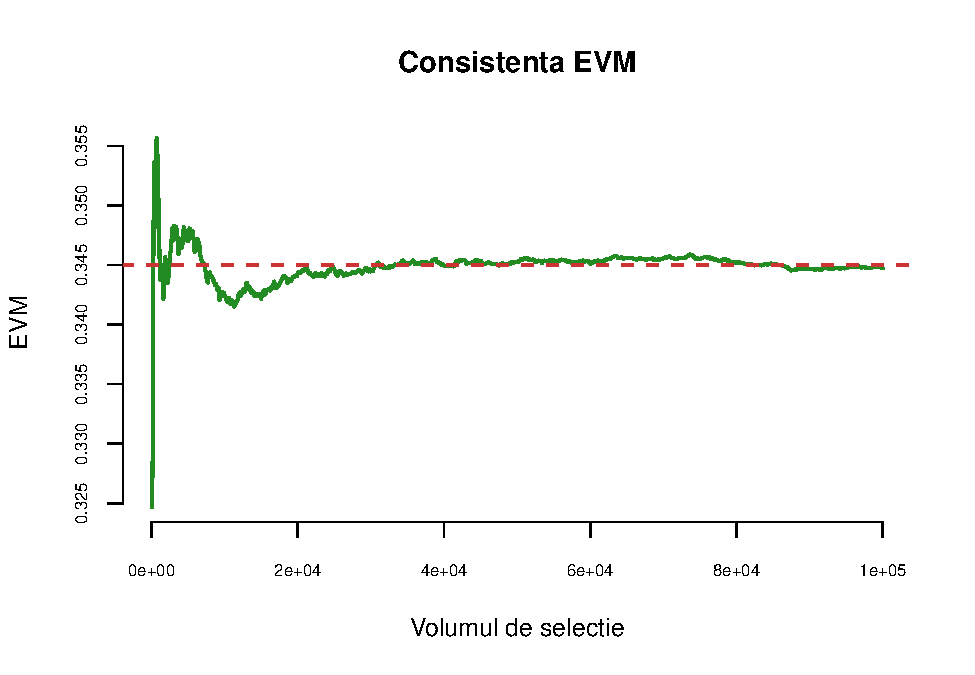
\includegraphics[width=0.8\linewidth]{Sem_1_files/figure-latex/unnamed-chunk-5-1} \end{center}

\subsection{Exemplu de EVM determinat prin soluții
numerice}\label{exemplu-de-evm-determinat-prin-solutii-numerice}

\begin{rmdexercise}
\marginnote{\enonce{12001}{}}\vspace{-7mm}

Fie \(X_1,X_2,\ldots,X_n\) un eșantion de talie \(n\) dintr-o populație
logistică a cărei densitate este dată de formula

\[
  f_{\theta}(x) = \frac{e^{-(x-\theta)}}{\left(1+e^{-(x-\theta)}\right)^2}, \quad x\in\mathbb{R},\, \theta\in\mathbb{R} 
\]

Determinați estimatorul de verosimilitate maximă \(\hat{\theta}_n\)
pentru \(\theta\).
\end{rmdexercise}

Densitatea de repartiție și funcția de repartiție a repartiției
logistice sunt ilustrate mai jos (în R se folosesc funcțiile:
\texttt{rlogis}, \texttt{dlogis}, \texttt{plogis} și respectiv
\texttt{qlogis}):

\begin{Shaded}
\begin{Highlighting}[]
\CommentTok{# Generam graficele }
\NormalTok{pars =}\StringTok{ }\KeywordTok{c}\NormalTok{(}\DecValTok{2}\NormalTok{, }\DecValTok{4}\NormalTok{, }\DecValTok{6}\NormalTok{, }\DecValTok{9}\NormalTok{)}

\NormalTok{x =}\StringTok{ }\KeywordTok{seq}\NormalTok{(}\OperatorTok{-}\DecValTok{8}\NormalTok{, }\DecValTok{15}\NormalTok{, }\DataTypeTok{length.out =} \DecValTok{250}\NormalTok{)}

\KeywordTok{set.seed}\NormalTok{(}\DecValTok{1234}\NormalTok{)}
\NormalTok{cols =}\StringTok{ }\KeywordTok{sample}\NormalTok{(}\KeywordTok{colors}\NormalTok{(), }\KeywordTok{length}\NormalTok{(pars))}

\KeywordTok{par}\NormalTok{(}\DataTypeTok{mfrow =} \KeywordTok{c}\NormalTok{(}\DecValTok{1}\NormalTok{, }\DecValTok{2}\NormalTok{))}
\CommentTok{# densitatile}
\KeywordTok{plot}\NormalTok{(x, }\KeywordTok{dlogis}\NormalTok{(x, }\DataTypeTok{location =}\NormalTok{ pars[}\DecValTok{1}\NormalTok{]),}
     \DataTypeTok{xlab =} \StringTok{"x"}\NormalTok{,}
     \DataTypeTok{ylab =} \KeywordTok{TeX}\NormalTok{(}\StringTok{"$f_\{}\CharTok{\textbackslash{}\textbackslash{}}\StringTok{theta\}(x)$"}\NormalTok{),}
     \CommentTok{# ylim = c(0,1),}
     \DataTypeTok{col =} \StringTok{"brown3"}\NormalTok{, }
     \DataTypeTok{lwd =} \DecValTok{2}\NormalTok{, }\DataTypeTok{type =} \StringTok{"l"}\NormalTok{,}
     \DataTypeTok{bty =} \StringTok{"n"}\NormalTok{,}
     \DataTypeTok{main =} \StringTok{"Densitatea"}\NormalTok{)}

\ControlFlowTok{for}\NormalTok{ (i }\ControlFlowTok{in} \KeywordTok{seq}\NormalTok{(}\KeywordTok{length}\NormalTok{(pars)}\OperatorTok{-}\DecValTok{1}\NormalTok{))\{}
\NormalTok{  location =}\StringTok{ }\NormalTok{pars[i}\OperatorTok{+}\DecValTok{1}\NormalTok{]}
    
\NormalTok{  y =}\StringTok{ }\KeywordTok{dlogis}\NormalTok{(x, }\DataTypeTok{location =}\NormalTok{ location)}
  
  \KeywordTok{lines}\NormalTok{(x, y, }\DataTypeTok{lwd =} \DecValTok{2}\NormalTok{, }
        \DataTypeTok{col =}\NormalTok{ cols[i])}
\NormalTok{\}}

\KeywordTok{legend}\NormalTok{(}\StringTok{"topright"}\NormalTok{, }
       \DataTypeTok{legend =} \KeywordTok{TeX}\NormalTok{(}\KeywordTok{paste0}\NormalTok{(}\StringTok{"$}\CharTok{\textbackslash{}\textbackslash{}}\StringTok{theta = "}\NormalTok{, pars, }\StringTok{"$"}\NormalTok{)),}
       \DataTypeTok{col =}\NormalTok{ cols,}
       \DataTypeTok{lwd =} \KeywordTok{rep}\NormalTok{(}\DecValTok{2}\NormalTok{, }\KeywordTok{length}\NormalTok{(pars)),}
       \DataTypeTok{bty =} \StringTok{"n"}\NormalTok{,}
       \DataTypeTok{cex =} \FloatTok{0.7}\NormalTok{,}
       \DataTypeTok{seg.len =} \FloatTok{1.5}\NormalTok{)}

\CommentTok{# functiile de repartitie}
\KeywordTok{plot}\NormalTok{(x, }\KeywordTok{plogis}\NormalTok{(x, }\DataTypeTok{location =}\NormalTok{ pars[}\DecValTok{1}\NormalTok{]),}
     \DataTypeTok{xlab =} \StringTok{"x"}\NormalTok{,}
     \DataTypeTok{ylab =} \KeywordTok{TeX}\NormalTok{(}\StringTok{"$F_\{}\CharTok{\textbackslash{}\textbackslash{}}\StringTok{theta\}(x)$"}\NormalTok{),}
     \DataTypeTok{ylim =} \KeywordTok{c}\NormalTok{(}\DecValTok{0}\NormalTok{,}\DecValTok{1}\NormalTok{),}
     \DataTypeTok{col =} \StringTok{"brown3"}\NormalTok{, }
     \DataTypeTok{lwd =} \DecValTok{2}\NormalTok{, }\DataTypeTok{type =} \StringTok{"l"}\NormalTok{,}
     \DataTypeTok{bty =} \StringTok{"n"}\NormalTok{,}
     \DataTypeTok{main =} \StringTok{"Functia de repartitie"}\NormalTok{)}

\ControlFlowTok{for}\NormalTok{ (i }\ControlFlowTok{in} \KeywordTok{seq}\NormalTok{(}\KeywordTok{length}\NormalTok{(pars)}\OperatorTok{-}\DecValTok{1}\NormalTok{))\{}
\NormalTok{  location =}\StringTok{ }\NormalTok{pars[i}\OperatorTok{+}\DecValTok{1}\NormalTok{]}
  
\NormalTok{  y =}\StringTok{ }\KeywordTok{plogis}\NormalTok{(x, }\DataTypeTok{location =}\NormalTok{ location)}
  
  \KeywordTok{lines}\NormalTok{(x, y, }\DataTypeTok{lwd =} \DecValTok{2}\NormalTok{, }
        \DataTypeTok{col =}\NormalTok{ cols[i])}
\NormalTok{\}}

\KeywordTok{legend}\NormalTok{(}\StringTok{"bottomright"}\NormalTok{, }
       \DataTypeTok{legend =} \KeywordTok{TeX}\NormalTok{(}\KeywordTok{paste0}\NormalTok{(}\StringTok{"$}\CharTok{\textbackslash{}\textbackslash{}}\StringTok{theta = "}\NormalTok{, pars, }\StringTok{"$"}\NormalTok{)),}
       \DataTypeTok{col =}\NormalTok{ cols,}
       \DataTypeTok{lwd =} \KeywordTok{rep}\NormalTok{(}\DecValTok{2}\NormalTok{, }\KeywordTok{length}\NormalTok{(pars)),}
       \DataTypeTok{bty =} \StringTok{"n"}\NormalTok{,}
       \DataTypeTok{cex =} \FloatTok{0.7}\NormalTok{,}
       \DataTypeTok{seg.len =} \FloatTok{1.5}\NormalTok{)}
\end{Highlighting}
\end{Shaded}

\begin{center}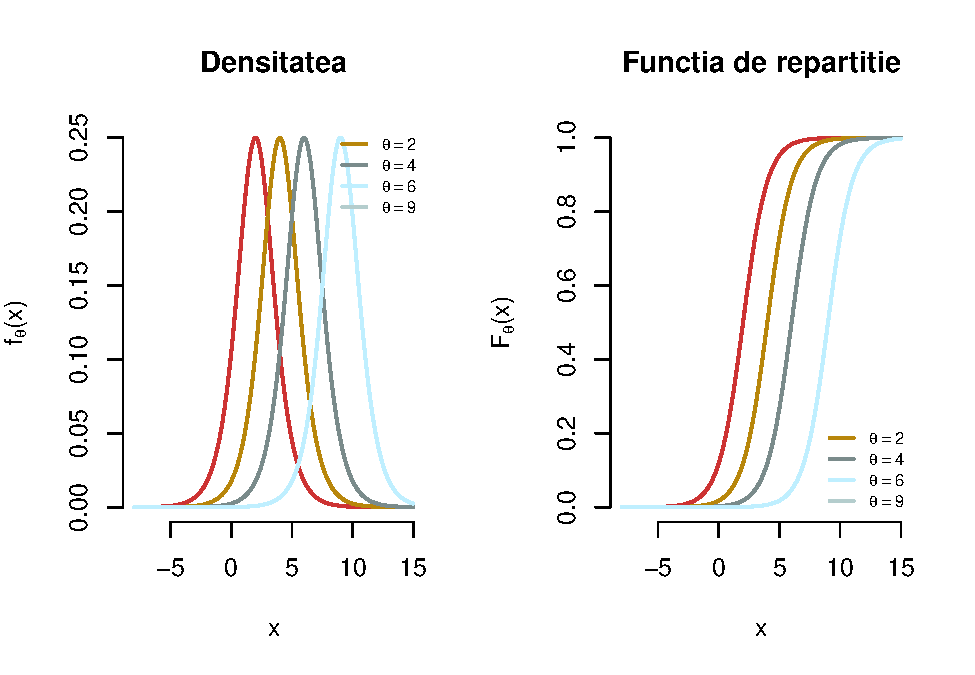
\includegraphics[width=0.7\linewidth]{Sem_1_files/figure-latex/unnamed-chunk-7-1} \end{center}

Observăm că funcția de verosimilitate este dată de

\[
L(\theta|\mathbf{x}) = \prod_{i=1}^{n}f_{\theta}(x_i) = \prod_{i=1}^{n}\frac{e^{-(x_i-\theta)}}{\left(1+e^{-(x_i-\theta)}\right)^2}
\]

iar logaritmul funcției de verosimilitate este

\[
l(\theta|\mathbf{x}) = \sum_{i=1}^{n}\log{f_{\theta}(x_i)} = n\theta - n\bar{x}_n - 2\sum_{i=1}^{n}\log{\left(1+e^{-(x_i-\theta)}\right)}.
\]

Pentru a găsi valoarea lui \(\theta\) care maximizează logaritmul
funcției de verosimilitate și prin urmare a funcției de verosimilitate
trebuie să rezolvăm ecuația \(l'(\theta|\mathbf{x}) = 0\), unde derivata
lui \(l(\theta|\mathbf{x})\) este

\[
l'(\theta|\mathbf{x}) = n - 2\sum_{i = 1}^{n}\frac{e^{-(x_i-\theta)}}{1+e^{-(x_i-\theta)}}
\]

ceea ce conduce la ecuația

\[
  \sum_{i = 1}^{n}\frac{e^{-(x_i-\theta)}}{1+e^{-(x_i-\theta)}} = \frac{n}{2} \tag{$\star$}
\]

Chiar dacă această ecuație nu se simplifică, se poate arăta că această
ecuația admite soluție unică. Observăm că derivata parțiala a membrului
drept în (\(\star\)) devine

\[
\frac{\partial }{\partial \theta}\sum_{i = 1}^{n}\frac{e^{-(x_i-\theta)}}{1+e^{-(x_i-\theta)}} = \sum_{i = 1}^{n}\frac{e^{-(x_i-\theta)}}{\left(1+e^{-(x_i-\theta)}\right)^2}>0
\]

ceea ce arată că membrul stâng este o funcție strict crescătoare în
\(\theta\). Cum membrul stâng în (\(\star\)) tinde spre \(0\) atunci
când \(\theta\to-\infty\) și spre \(n\) pentru \(\theta\to\infty\)
deducem că ecuația (\(\star\)) admite soluție unică (vezi graficul de
mai jos).

\begin{Shaded}
\begin{Highlighting}[]
\KeywordTok{set.seed}\NormalTok{(}\DecValTok{112}\NormalTok{)}
\NormalTok{n =}\StringTok{ }\DecValTok{20}
\NormalTok{x =}\StringTok{ }\KeywordTok{rlogis}\NormalTok{(n, }\DataTypeTok{location =} \FloatTok{7.5}\NormalTok{)}

\CommentTok{# derivata logaritmului functiei de verosimilitate}
\NormalTok{dLogLogistic =}\StringTok{ }\ControlFlowTok{function}\NormalTok{(n, x, theta)\{}
  \KeywordTok{sapply}\NormalTok{(theta, }\ControlFlowTok{function}\NormalTok{(t)\{}
\NormalTok{    y =}\StringTok{ }\KeywordTok{exp}\NormalTok{(}\OperatorTok{-}\NormalTok{(x }\OperatorTok{-}\StringTok{ }\NormalTok{t))}
\NormalTok{    n }\OperatorTok{-}\StringTok{ }\DecValTok{2}\OperatorTok{*}\KeywordTok{sum}\NormalTok{(y}\OperatorTok{/}\NormalTok{(}\DecValTok{1}\OperatorTok{+}\NormalTok{y))}
\NormalTok{  \})}
\NormalTok{\}}

\NormalTok{theta =}\StringTok{ }\KeywordTok{seq}\NormalTok{(}\DecValTok{0}\NormalTok{, }\DecValTok{15}\NormalTok{, }\DataTypeTok{length.out =} \DecValTok{250}\NormalTok{)}

\NormalTok{mar.default <-}\StringTok{ }\KeywordTok{c}\NormalTok{(}\DecValTok{5}\NormalTok{,}\DecValTok{4}\NormalTok{,}\DecValTok{4}\NormalTok{,}\DecValTok{2}\NormalTok{) }\OperatorTok{+}\StringTok{ }\FloatTok{0.1}
\KeywordTok{par}\NormalTok{(}\DataTypeTok{mar =}\NormalTok{ mar.default }\OperatorTok{+}\StringTok{ }\KeywordTok{c}\NormalTok{(}\DecValTok{0}\NormalTok{, }\FloatTok{1.2}\NormalTok{, }\DecValTok{0}\NormalTok{, }\DecValTok{0}\NormalTok{))}

\KeywordTok{plot}\NormalTok{(theta, }\KeywordTok{dLogLogistic}\NormalTok{(n, x, theta), }\DataTypeTok{type =} \StringTok{"l"}\NormalTok{,}
     \DataTypeTok{col =} \StringTok{"forestgreen"}\NormalTok{, }\DataTypeTok{lwd =} \DecValTok{2}\NormalTok{,}
     \DataTypeTok{bty =} \StringTok{"n"}\NormalTok{,}
     \DataTypeTok{xlab =} \KeywordTok{TeX}\NormalTok{(}\StringTok{"$}\CharTok{\textbackslash{}\textbackslash{}}\StringTok{theta$"}\NormalTok{),}
     \DataTypeTok{ylab =} \KeywordTok{TeX}\NormalTok{(}\StringTok{"$}\CharTok{\textbackslash{}\textbackslash{}}\StringTok{frac\{}\CharTok{\textbackslash{}\textbackslash{}}\StringTok{partial\}\{}\CharTok{\textbackslash{}\textbackslash{}}\StringTok{partial }\CharTok{\textbackslash{}\textbackslash{}}\StringTok{theta\} l(}\CharTok{\textbackslash{}\textbackslash{}}\StringTok{theta | x)$"}\NormalTok{))}

\KeywordTok{abline}\NormalTok{(}\DataTypeTok{h =} \DecValTok{0}\NormalTok{, }\DataTypeTok{col =} \StringTok{"brown3"}\NormalTok{,}
       \DataTypeTok{lty =} \DecValTok{2}\NormalTok{)}
\end{Highlighting}
\end{Shaded}

\begin{center}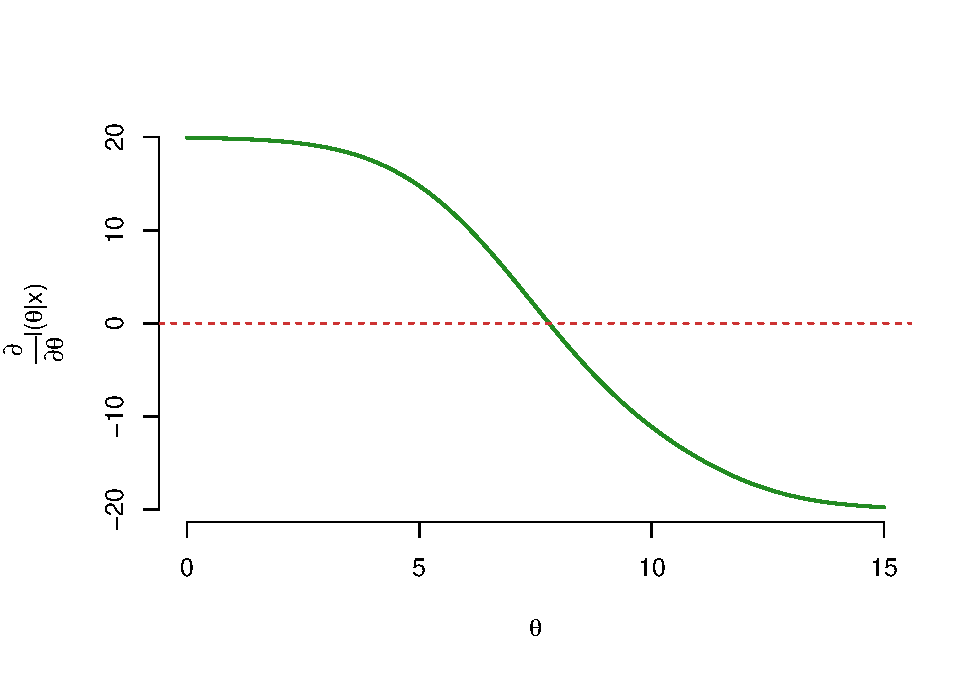
\includegraphics[width=0.7\linewidth]{Sem_1_files/figure-latex/unnamed-chunk-8-1} \end{center}

Cum nu putem găsi o soluție a ecuației \(l'(\theta|\mathbf{x}) = 0\) sub
formă compactă, este necesar să apelăm la metode numerice. O astfel de
metodă numerică este binecunoscuta
\href{https://en.wikipedia.org/wiki/Newton\%27s_method}{metodă a lui
Newton-Raphson}. Metoda presupune să începem cu o valoare (soluție)
inițială \(\hat{\theta}^{(0)}\) și să alegem, plecând de la aceasta, o
nouă valoare \(\hat{\theta}^{(1)}\) definită prin

\[
  \hat{\theta}^{(1)} = \hat{\theta}^{(0)} - \frac{l'\left(\hat{\theta}^{(0)}\right)}{l''\left(\hat{\theta}^{(0)}\right)},
\]

adică \(\hat{\theta}^{(1)}\) este intersecția cu axa absciselor a
tangentei în punctul
\(\left(\hat{\theta}^{(0)}, l'\left(\hat{\theta}^{(0)}\right)\right)\)
la graficul funcției \(l'(\theta)\). Ideea este de a itera procesul până
când soluția converge, cu alte cuvinte pornind de la o valoare
\emph{rezonabilă} de start \(\hat{\theta}^{(0)}\) la pasul \(k+1\) avem

\[
  \hat{\theta}^{(k+1)} = \hat{\theta}^{(k)} - \frac{l'\left(\hat{\theta}^{(k)}\right)}{l''\left(\hat{\theta}^{(k)}\right)}
\]

și oprim procesul atunco când \(k\) este suficient de mare și/sau
\(\left|\hat{\theta}^{(k+1)} - \hat{\theta}^{(k)}\right|\) este
suficient de mic. Următorul grafic ilustrează grafic algoritmul lui
Newton:

\begin{Shaded}
\begin{Highlighting}[]
\KeywordTok{set.seed}\NormalTok{(}\DecValTok{112}\NormalTok{)}
\NormalTok{n =}\StringTok{ }\DecValTok{20}
\NormalTok{x =}\StringTok{ }\KeywordTok{rlogis}\NormalTok{(n, }\DataTypeTok{location =} \FloatTok{7.5}\NormalTok{)}

\CommentTok{# derivata logaritmului functiei de verosimilitate}
\NormalTok{dLogLogistic =}\StringTok{ }\ControlFlowTok{function}\NormalTok{(n, x, theta)\{}
  \KeywordTok{sapply}\NormalTok{(theta, }\ControlFlowTok{function}\NormalTok{(t)\{}
\NormalTok{    y =}\StringTok{ }\KeywordTok{exp}\NormalTok{(}\OperatorTok{-}\NormalTok{(x }\OperatorTok{-}\StringTok{ }\NormalTok{t))}
\NormalTok{    n }\OperatorTok{-}\StringTok{ }\DecValTok{2}\OperatorTok{*}\KeywordTok{sum}\NormalTok{(y}\OperatorTok{/}\NormalTok{(}\DecValTok{1}\OperatorTok{+}\NormalTok{y))}
\NormalTok{  \})}
\NormalTok{\}}

\NormalTok{theta =}\StringTok{ }\KeywordTok{seq}\NormalTok{(}\DecValTok{0}\NormalTok{, }\DecValTok{15}\NormalTok{, }\DataTypeTok{length.out =} \DecValTok{250}\NormalTok{)}

\NormalTok{mar.default <-}\StringTok{ }\KeywordTok{c}\NormalTok{(}\DecValTok{5}\NormalTok{,}\DecValTok{4}\NormalTok{,}\DecValTok{4}\NormalTok{,}\DecValTok{2}\NormalTok{) }\OperatorTok{+}\StringTok{ }\FloatTok{0.1}
\KeywordTok{par}\NormalTok{(}\DataTypeTok{mar =}\NormalTok{ mar.default }\OperatorTok{+}\StringTok{ }\KeywordTok{c}\NormalTok{(}\DecValTok{0}\NormalTok{, }\FloatTok{1.2}\NormalTok{, }\DecValTok{0}\NormalTok{, }\DecValTok{0}\NormalTok{))}

\KeywordTok{plot}\NormalTok{(theta, }\KeywordTok{dLogLogistic}\NormalTok{(n, x, theta), }\DataTypeTok{type =} \StringTok{"l"}\NormalTok{,}
     \DataTypeTok{col =} \StringTok{"forestgreen"}\NormalTok{, }\DataTypeTok{lwd =} \DecValTok{2}\NormalTok{,}
     \DataTypeTok{bty =} \StringTok{"n"}\NormalTok{,}
     \DataTypeTok{xlab =} \KeywordTok{TeX}\NormalTok{(}\StringTok{"$}\CharTok{\textbackslash{}\textbackslash{}}\StringTok{theta$"}\NormalTok{),}
     \DataTypeTok{ylab =} \KeywordTok{TeX}\NormalTok{(}\StringTok{"$}\CharTok{\textbackslash{}\textbackslash{}}\StringTok{frac\{}\CharTok{\textbackslash{}\textbackslash{}}\StringTok{partial\}\{}\CharTok{\textbackslash{}\textbackslash{}}\StringTok{partial }\CharTok{\textbackslash{}\textbackslash{}}\StringTok{theta\} l(}\CharTok{\textbackslash{}\textbackslash{}}\StringTok{theta | x)$"}\NormalTok{))}

\KeywordTok{abline}\NormalTok{(}\DataTypeTok{h =} \DecValTok{0}\NormalTok{, }\DataTypeTok{col =} \StringTok{"brown3"}\NormalTok{,}
       \DataTypeTok{lty =} \DecValTok{2}\NormalTok{)}

\CommentTok{# ilustrarea metodei Newton}

\NormalTok{dl =}\StringTok{ }\ControlFlowTok{function}\NormalTok{(theta) n }\OperatorTok{-}\StringTok{ }\DecValTok{2} \OperatorTok{*}\StringTok{ }\KeywordTok{sum}\NormalTok{(}\KeywordTok{exp}\NormalTok{(theta }\OperatorTok{-}\StringTok{ }\NormalTok{x) }\OperatorTok{/}\StringTok{ }\NormalTok{(}\DecValTok{1} \OperatorTok{+}\StringTok{ }\KeywordTok{exp}\NormalTok{(theta }\OperatorTok{-}\StringTok{ }\NormalTok{x)))}
\NormalTok{ddl =}\StringTok{ }\ControlFlowTok{function}\NormalTok{(theta) \{}\OperatorTok{-}\DecValTok{2} \OperatorTok{*}\StringTok{ }\KeywordTok{sum}\NormalTok{(}\KeywordTok{exp}\NormalTok{(theta }\OperatorTok{-}\StringTok{ }\NormalTok{x) }\OperatorTok{/}\StringTok{ }\NormalTok{(}\DecValTok{1} \OperatorTok{+}\StringTok{ }\KeywordTok{exp}\NormalTok{(theta }\OperatorTok{-}\StringTok{ }\NormalTok{x))}\OperatorTok{^}\DecValTok{2}\NormalTok{)\}}

\NormalTok{x0 =}\StringTok{ }\DecValTok{5} \CommentTok{# punctul de start}

\KeywordTok{points}\NormalTok{(x0, }\DecValTok{0}\NormalTok{, }\DataTypeTok{pch =} \DecValTok{16}\NormalTok{, }\DataTypeTok{col =} \StringTok{"black"}\NormalTok{)}
\KeywordTok{text}\NormalTok{(x0, }\DecValTok{0}\NormalTok{, }\DataTypeTok{labels =} \KeywordTok{TeX}\NormalTok{(}\StringTok{"$}\CharTok{\textbackslash{}\textbackslash{}}\StringTok{hat\{}\CharTok{\textbackslash{}\textbackslash{}}\StringTok{theta\}^\{(0)\}$"}\NormalTok{), }\DataTypeTok{pos =} \DecValTok{1}\NormalTok{, }\DataTypeTok{cex =} \FloatTok{0.8}\NormalTok{)}
\KeywordTok{segments}\NormalTok{(x0, }\DecValTok{0}\NormalTok{, x0, }\KeywordTok{dl}\NormalTok{(x0), }\DataTypeTok{lty =} \DecValTok{2}\NormalTok{, }\DataTypeTok{col =} \StringTok{"grey50"}\NormalTok{)}
\KeywordTok{points}\NormalTok{(x0, }\KeywordTok{dl}\NormalTok{(x0), }\DataTypeTok{pch =} \DecValTok{4}\NormalTok{)}

\NormalTok{x1 =}\StringTok{ }\NormalTok{x0 }\OperatorTok{-}\StringTok{ }\KeywordTok{dl}\NormalTok{(x0)}\OperatorTok{/}\KeywordTok{ddl}\NormalTok{(x0)}

\KeywordTok{segments}\NormalTok{(x0, }\KeywordTok{dl}\NormalTok{(x0), x1, }\DecValTok{0}\NormalTok{, }\DataTypeTok{lty =} \DecValTok{1}\NormalTok{, }\DataTypeTok{lwd =} \DecValTok{2}\NormalTok{, }\DataTypeTok{col =} \StringTok{"grey50"}\NormalTok{)}
\KeywordTok{points}\NormalTok{(x1, }\DecValTok{0}\NormalTok{, }\DataTypeTok{pch =} \DecValTok{16}\NormalTok{, }\DataTypeTok{col =} \StringTok{"black"}\NormalTok{)}
\KeywordTok{text}\NormalTok{(x1, }\DecValTok{0}\NormalTok{, }\DataTypeTok{labels =} \KeywordTok{TeX}\NormalTok{(}\StringTok{"$}\CharTok{\textbackslash{}\textbackslash{}}\StringTok{hat\{}\CharTok{\textbackslash{}\textbackslash{}}\StringTok{theta\}^\{(1)\}$"}\NormalTok{), }\DataTypeTok{pos =} \DecValTok{1}\NormalTok{, }\DataTypeTok{cex =} \FloatTok{0.8}\NormalTok{)}
\KeywordTok{segments}\NormalTok{(x1, }\DecValTok{0}\NormalTok{, x1, }\KeywordTok{dl}\NormalTok{(x1), }\DataTypeTok{lty =} \DecValTok{2}\NormalTok{, }\DataTypeTok{col =} \StringTok{"grey50"}\NormalTok{)}
\KeywordTok{points}\NormalTok{(x1, }\KeywordTok{dl}\NormalTok{(x1), }\DataTypeTok{pch =} \DecValTok{4}\NormalTok{)}

\NormalTok{x2 =}\StringTok{ }\NormalTok{x1 }\OperatorTok{-}\StringTok{ }\KeywordTok{dl}\NormalTok{(x1)}\OperatorTok{/}\KeywordTok{ddl}\NormalTok{(x1)}

\KeywordTok{segments}\NormalTok{(x1, }\KeywordTok{dl}\NormalTok{(x1), x2, }\DecValTok{0}\NormalTok{, }\DataTypeTok{lty =} \DecValTok{1}\NormalTok{, }\DataTypeTok{lwd =} \DecValTok{2}\NormalTok{, }\DataTypeTok{col =} \StringTok{"grey50"}\NormalTok{)}
\KeywordTok{points}\NormalTok{(x2, }\DecValTok{0}\NormalTok{, }\DataTypeTok{pch =} \DecValTok{16}\NormalTok{, }\DataTypeTok{col =} \StringTok{"black"}\NormalTok{)}
\KeywordTok{text}\NormalTok{(x2, }\DecValTok{0}\NormalTok{, }\DataTypeTok{labels =} \KeywordTok{TeX}\NormalTok{(}\StringTok{"$}\CharTok{\textbackslash{}\textbackslash{}}\StringTok{hat\{}\CharTok{\textbackslash{}\textbackslash{}}\StringTok{theta\}^\{(2)\}$"}\NormalTok{), }\DataTypeTok{pos =} \DecValTok{1}\NormalTok{, }\DataTypeTok{cex =} \FloatTok{0.8}\NormalTok{)}
\end{Highlighting}
\end{Shaded}

\begin{center}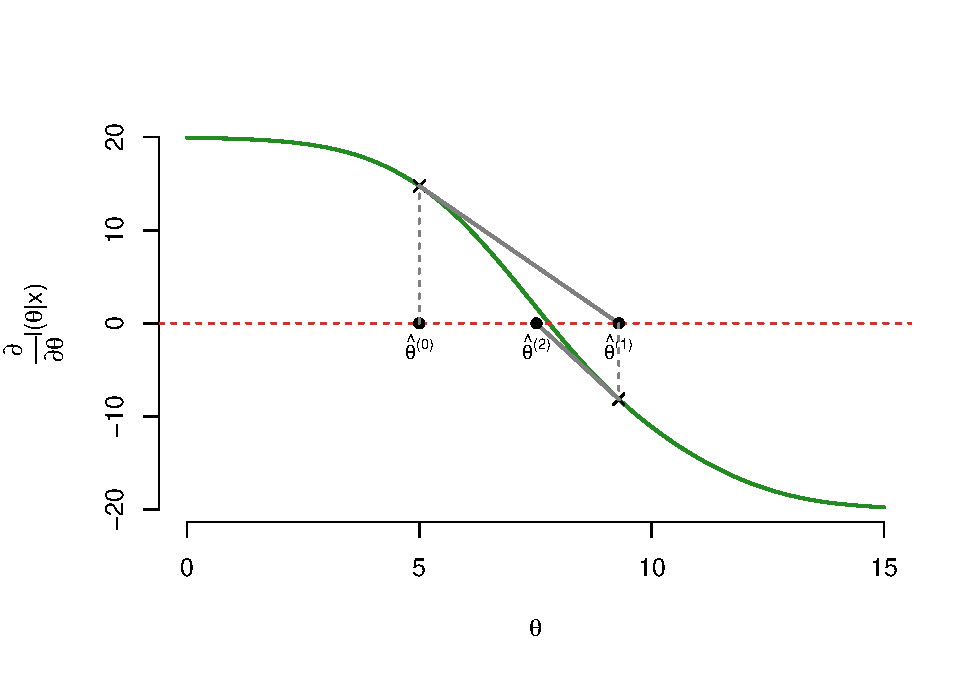
\includegraphics[width=0.7\linewidth]{Sem_1_files/figure-latex/unnamed-chunk-9-1} \end{center}

\textbf{Obs:} Singurul lucru care se schimbă atunci când trecem de la
scalar la vector, este funcția \(l(\theta)\) care acum este o funcție de
\(p>1\) variabile,
\(\theta = (\theta_1, \theta_2, \ldots, \theta_p)^{\intercal}\in\mathbb{R}^p\).
În acest context \(l'(\theta)\) este un vector de derivate parțiale iar
\(l''(\theta)\) este o matrice de derivate parțiale de ordin doi. Prin
urmare itarațiile din metoda lui Newton sunt

\[
  \hat{\theta}^{(k+1)} = \hat{\theta}^{(k)} - \left[l''\left(\hat{\theta}^{(k)}\right)\right]^{-1}l'\left(\hat{\theta}^{(k)}\right)
\] unde \([\cdot]^{-1}\) este
\href{https://en.wikipedia.org/wiki/Moore\%E2\%80\%93Penrose_inverse}{pseudoinversa}
unei matrici.

Funcția de mai jos implementează metoada lui Newton pentru cazul
multidimensional:

\begin{Shaded}
\begin{Highlighting}[]
\CommentTok{# Metoda lui Newton}

\NormalTok{newton <-}\StringTok{ }\ControlFlowTok{function}\NormalTok{(f, df, x0, }\DataTypeTok{eps=}\FloatTok{1e-08}\NormalTok{, }\DataTypeTok{maxiter=}\DecValTok{1000}\NormalTok{, ...) \{}
  \CommentTok{# in caz ca nu e incarcat pachetul sa putem accesa pseudoinversa}
  \ControlFlowTok{if}\NormalTok{(}\OperatorTok{!}\KeywordTok{exists}\NormalTok{(}\StringTok{"ginv"}\NormalTok{)) }\KeywordTok{library}\NormalTok{(MASS) }
  
\NormalTok{  x <-}\StringTok{ }\NormalTok{x0}
\NormalTok{  k <-}\StringTok{ }\DecValTok{0}
  
  \ControlFlowTok{repeat}\NormalTok{ \{}
\NormalTok{    k <-}\StringTok{ }\NormalTok{k }\OperatorTok{+}\StringTok{ }\DecValTok{1}
    
\NormalTok{    x.new <-}\StringTok{ }\NormalTok{x }\OperatorTok{-}\StringTok{ }\KeywordTok{as.numeric}\NormalTok{(}\KeywordTok{ginv}\NormalTok{(}\KeywordTok{df}\NormalTok{(x, ...)) }\OperatorTok\StringTok{ }\KeywordTok{f}\NormalTok{(x, ...))}
    
    \ControlFlowTok{if}\NormalTok{(}\KeywordTok{mean}\NormalTok{(}\KeywordTok{abs}\NormalTok{(x.new }\OperatorTok{-}\StringTok{ }\NormalTok{x)) }\OperatorTok{<}\StringTok{ }\NormalTok{eps }\OperatorTok{|}\StringTok{ }\NormalTok{k }\OperatorTok{>=}\StringTok{ }\NormalTok{maxiter) \{}
      \ControlFlowTok{if}\NormalTok{(k }\OperatorTok{>=}\StringTok{ }\NormalTok{maxiter) }\KeywordTok{warning}\NormalTok{(}\StringTok{"S-a atins numarul maxim de iteratii!"}\NormalTok{)}
      \ControlFlowTok{break}
\NormalTok{    \}}
\NormalTok{    x <-}\StringTok{ }\NormalTok{x.new}
\NormalTok{  \}}
\NormalTok{  out <-}\StringTok{ }\KeywordTok{list}\NormalTok{(}\DataTypeTok{solution =}\NormalTok{ x.new, }\DataTypeTok{value =} \KeywordTok{f}\NormalTok{(x.new, ...), }\DataTypeTok{iter =}\NormalTok{ k)}
  
  \KeywordTok{return}\NormalTok{(out)}
\NormalTok{\}}
\end{Highlighting}
\end{Shaded}

Să presupunem că am observat următorul eșantion de talie \(20\) din
repartiția logistică:

\begin{verbatim}
 [1]  6.996304  9.970107 12.304991 11.259549  6.326912  5.378941  4.299639
 [8]  8.484635  5.601117  7.094335  6.324731  6.868456  9.753360  8.042095
[15]  8.227830 10.977982  7.743096  7.722159  8.562884  6.968356
\end{verbatim}

\begin{Shaded}
\begin{Highlighting}[]
\KeywordTok{set.seed}\NormalTok{(}\DecValTok{112}\NormalTok{)}
\NormalTok{x =}\StringTok{ }\KeywordTok{rlogis}\NormalTok{(}\DecValTok{20}\NormalTok{, }\DataTypeTok{location =} \FloatTok{7.5}\NormalTok{)}

\NormalTok{n =}\StringTok{ }\KeywordTok{length}\NormalTok{(x)}
\NormalTok{dl =}\StringTok{ }\ControlFlowTok{function}\NormalTok{(theta) n }\OperatorTok{-}\StringTok{ }\DecValTok{2} \OperatorTok{*}\StringTok{ }\KeywordTok{sum}\NormalTok{(}\KeywordTok{exp}\NormalTok{(theta }\OperatorTok{-}\StringTok{ }\NormalTok{x) }\OperatorTok{/}\StringTok{ }\NormalTok{(}\DecValTok{1} \OperatorTok{+}\StringTok{ }\KeywordTok{exp}\NormalTok{(theta }\OperatorTok{-}\StringTok{ }\NormalTok{x)))}
\NormalTok{ddl =}\StringTok{ }\ControlFlowTok{function}\NormalTok{(theta) \{}\OperatorTok{-}\DecValTok{2} \OperatorTok{*}\StringTok{ }\KeywordTok{sum}\NormalTok{(}\KeywordTok{exp}\NormalTok{(theta }\OperatorTok{-}\StringTok{ }\NormalTok{x) }\OperatorTok{/}\StringTok{ }\NormalTok{(}\DecValTok{1} \OperatorTok{+}\StringTok{ }\KeywordTok{exp}\NormalTok{(theta }\OperatorTok{-}\StringTok{ }\NormalTok{x))}\OperatorTok{^}\DecValTok{2}\NormalTok{)\}}

\NormalTok{logis.newton =}\StringTok{ }\KeywordTok{newton}\NormalTok{(dl, ddl, }\KeywordTok{median}\NormalTok{(x))}
\end{Highlighting}
\end{Shaded}

și aplicănd metoda lui Newton găsim estimatorul de verosimilitate maximă
\(\hat{\theta}_n=\) 7.7933 după numai 3 iterații (datele au fost
simulate folosind \(\theta = 7.5\)).

\subsection{\texorpdfstring{Metoda verosimilității maxime și procese
autoregresive
\(AR(r)\)}{Metoda verosimilității maxime și procese autoregresive AR(r)}}\label{metoda-verosimilitatii-maxime-si-procese-autoregresive-arr}

\begin{rmdexercise}
\marginnote{\enonce{13001}{}}\vspace{-7mm}

Se numește proces autoregresiv de ordin 1 \(AR(1)\), un proces Gaussian
staționar definit prin

\[
  Y_t = c + \rho Y_{t-1} + \epsilon_{t}
\]

cu \(\epsilon_{t}\) variabile aleatoare i.i.d. repartizate
\(\mathcal{N}(0,\sigma^2)\) și \(|\rho|<1\).
\end{rmdexercise}

Observăm că din condiția de staționaritate\footnote{Aici ne referim la
  proprietatea de staționaritate în sens larg (wide-sense stationary)
  care presupune că \(\forall t_1,t_2\in\mathbb{N}\) și
  \(\forall \tau\in\mathbb{N}\) avem
  \(\mathbb{E}[Y_{t_1}] = \mathbb{E}[Y_{t_2}]\) și
  \(\mathbb{E}[Y_{t_1}Y_{t_2}] = \mathbb{E}[Y_{t_1+\tau}Y_{t_2+\tau}]\).}
rezultă că

\[
  \mathbb{E}[Y_t] = \frac{c}{1-\rho} ,\quad Var[Y_t] = \frac{\sigma^2}{1-\rho^2}.
\]

\begin{rmdexercise}
\marginnote{\enonce{13002}{}}\vspace{-7mm}

Fie \(\boldsymbol{\theta} = (c, \rho, \sigma^2)^\intercal\) vectorul
parametrilor modelului. Scrieți funcția de verosimilitate și logaritmul
funcției de verosimilitae pentru o observație, \(y_1\).
\end{rmdexercise}

Cum variabila aleatoare \(Y_1\) are media și varianța date de

\[
  \mathbb{E}[Y_1] = \frac{c}{1-\rho} ,\quad Var[Y_1] = \frac{\sigma^2}{1-\rho^2}.
\]

iar \(\epsilon_t\) sunt i.i.d. repartizate \(\mathcal{N}(0,\sigma^2)\),
deducem că \(Y_1\) este repartizată tot normal, cu
\(Y_1\sim\mathcal{N}\left(\frac{c}{1-\rho}, \frac{\sigma^2}{1-\rho^2}\right)\).
Astfel funcția de verosimilitate pentru \(y_1\) este

\[
  L(\boldsymbol{\theta};y_1) = \frac{1}{\sqrt{2\pi}\sqrt{\frac{\sigma^2}{1-\rho^2}}}e^{-\frac{1}{2}\frac{\left(y_1 - \frac{c}{1-\rho}\right)^2}{\frac{\sigma^2}{1-\rho^2}}}
\]

iar logaritmul funcției de verosimilitate pentru \(y_1\) este

\[
  l(\boldsymbol{\theta};y_1) = -\frac{1}{2}\log(2\pi) - \frac{1}{2}\log\left(\frac{\sigma^2}{1-\rho^2}\right) -\frac{1}{2}\frac{\left(y_1 - \frac{c}{1-\rho}\right)^2}{\frac{\sigma^2}{1-\rho^2}}.
\]

\begin{rmdexercise}
\marginnote{\enonce{13003}{}}\vspace{-7mm}

Care este repartiția condiționată a lui \(Y_2\) la \(Y_1 = y_1\)?
Scrieți funcția de verosimilitate și logaritmul funcției de
verosimilitate (condiționată) pentru a doua observație \(y_2\).
\end{rmdexercise}

Observăm că pentru \(t=2\) avem

\[
  Y_2 = c + \rho Y_1 + \epsilon_2,
\]

unde \(\epsilon_2\sim\mathcal{N}(0,\sigma^2)\). Prin urmare repartiția
condiționată a lui \(Y_2\) dat fiind \(Y_1 = y_1\) este

\[
  Y_2|Y_1=y_1\sim\mathcal{N}(c+\rho y_1,\sigma^2)
\]

de unde funcția de verosimilitate (condiționată) pentru \(y_2\) este

\[
  L(\boldsymbol{\theta};y_2|y_1) = f_{Y_2|Y_1}(y_2|y_1;\boldsymbol{\theta}) = \frac{1}{\sigma\sqrt{2\pi}}e^{-\frac{1}{2}\frac{\left(y_2 - c-\rho y_1\right)^2}{\sigma^2}}
\]

iar logaritmul funcției de verosimilitate (condiționată) pentru \(y_2\)
este

\[
  l(\boldsymbol{\theta};y_2|y_1) = \log f_{Y_2|Y_1}(y_2|y_1;\boldsymbol{\theta}) = -\frac{1}{2}\log(2\pi) - \frac{1}{2}\log\left(\sigma^2\right)-\frac{1}{2}\frac{\left(y_2 - c-\rho y_1\right)^2}{\sigma^2}.
\]

\begin{rmdexercise}
\marginnote{\enonce{13004}{}}\vspace{-7mm}

Considerați eșantionul \(\{y_1, y_2\}\) de talie \(2\). Scrieți funcția
de verosimilitate (completă) și logaritmul funcției de verosimilitate a
modelului \(AR(1)\) pentru acest eșantion. Extindeți rezultatul pentru
un eșantion \(y_1,y_2,\ldots,y_T\) de talie \(T\).
\end{rmdexercise}

Reamintim că dacă avem două variabile aleatoare continue (absolut
continue) \(X\) și \(Y\) atunci densitatea cuplului \((X,Y)\) este

\[
  f_{(X,Y)}(x,y) = f_{Y|X}(y|x)f_{X}(x),
\]

prin urmare funcția de verosimilitate (completă) pentru eșantionul
\(\{y_1, y_2\}\) este

\[
  L(\boldsymbol{\theta};y_1,y_2) = f_{(Y_1,Y_2)}(y_1,y_2;\boldsymbol{\theta}) = f_{Y_2|Y_1}(y_2|y_1;\boldsymbol{\theta})f_{Y_1}(y_1;\boldsymbol{\theta})
\]

sau echivalent

\[
  L(\boldsymbol{\theta};y_1,y_2) = L(\boldsymbol{\theta};y_2|y_1)L(\boldsymbol{\theta};y_1) = \frac{\sqrt{1-\rho^2}}{2 \pi\sigma^2}e^{-\frac{1}{2}\frac{(1-\rho^2)\left(y_1 - \frac{c}{1-\rho}\right)^2}{\sigma^2}-\frac{1}{2}\frac{\left(y_2 - c-\rho y_1\right)^2}{\sigma^2}}.
\]

În mod similar, logaritmul funcției de verosimilitate este

\[
  l(\boldsymbol{\theta};y_1,y_2) = l(\boldsymbol{\theta};y_2|y_1)+ l(\boldsymbol{\theta};y_1) = \frac{1}{2}\log(1-\rho^2) - \log(2 \pi\sigma^2) -\frac{1}{2}\frac{(1-\rho^2)\left(y_1 - \frac{c}{1-\rho}\right)^2}{\sigma^2}-\frac{1}{2}\frac{\left(y_2 - c-\rho y_1\right)^2}{\sigma^2}.
\] Observăm că densitatea lui \(Y_3\) condiționată la primele două
variabile este

\[
  f_{Y_3|Y_2,Y_1}(y_3|y_2, y_1;\boldsymbol{\theta}) = \frac{1}{\sigma\sqrt{2\pi}}e^{-\frac{1}{2}\frac{(y_3 - c -\rho y_2)^2}{\sigma^2}}
\]

de unde

\begin{align*}
  f_{Y_3, Y_2, Y_1}(y_3, y_2, y_1;\boldsymbol{\theta}) &= f_{Y_3|Y_2,Y_1}(y_3|y_2, y_1;\boldsymbol{\theta})f_{Y_2,Y_1}(y_2, y_1;\boldsymbol{\theta})\\
  &= f_{Y_3|Y_2,Y_1}(y_3|y_2, y_1;\boldsymbol{\theta})f_{Y_2|Y_1}(y_2|y_1;\boldsymbol{\theta})f_{Y_1}(y_1;\boldsymbol{\theta}).
\end{align*}

În general, valoarea lui \(Y_1, Y_2, \ldots, Y_{t-1}\) influențează
valoarea lui \(Y_{t}\) doar prin valoarea lui \(Y_{t-1}\) ceea ce arată
că densitatea lui \(Y_{t}\) condiționată la celelalte \(t-1\) variabile
este

\[
  f_{Y_t|Y_{t-1}, Y_{t-2},\ldots, Y_1}(y_t|y_{t-1}, y_{t-2},\ldots, y_1;\boldsymbol{\theta}) = f_{Y_t|Y_{t-1}}(y_t|y_{t-1};\boldsymbol{\theta}) = \frac{1}{\sigma\sqrt{2\pi}}e^{-\frac{1}{2}\frac{(y_t - c -\rho y_{t-1})^2}{\sigma^2}}.
\]

Astfel, pentru un eșantion \(y_1,y_2,\ldots,y_T\) de talie \(T\) avem

\begin{align*}
 L(\boldsymbol{\theta};y_1,y_2,\ldots,y_T) &= L(\boldsymbol{\theta};y_1)\times\prod_{t = 2}^{T}L(\boldsymbol{\theta};y_t|y_{t-1})\\
 l(\boldsymbol{\theta};y_1,y_2,\ldots,y_T) &= l(\boldsymbol{\theta};y_1)+\sum_{t = 2}^{T}l(\boldsymbol{\theta};y_t|y_{t-1})
\end{align*}

ceea ce conduce la

\begin{align*}
 L(\boldsymbol{\theta};y_1,y_2,\ldots,y_T) &= \frac{1}{\sqrt{2\pi}\sqrt{\frac{\sigma^2}{1-\rho^2}}}e^{-\frac{1}{2}\frac{\left(y_1 - \frac{c}{1-\rho}\right)^2}{\frac{\sigma^2}{1-\rho^2}}}\times\prod_{t = 2}^{T}\frac{1}{\sigma\sqrt{2\pi}}e^{-\frac{1}{2}\frac{\left(y_t - c-\rho y_{t-1}\right)^2}{\sigma^2}}
\end{align*}

și respectiv la

\begin{align*}
 l(\boldsymbol{\theta};y_1,y_2,\ldots,y_T) &= -\frac{1}{2}\log(2\pi) - \frac{1}{2}\log\left(\frac{\sigma^2}{1-\rho^2}\right) -\frac{1}{2}\frac{\left(y_1 - \frac{c}{1-\rho}\right)^2}{\frac{\sigma^2}{1-\rho^2}}\\
       &\quad +\sum_{t = 2}^{T}\left(-\frac{1}{2}\log(2\pi) - \frac{1}{2}\log\left(\sigma^2\right)-\frac{1}{2}\frac{\left(y_t - c-\rho y_{t-1}\right)^2}{\sigma^2}\right)\\
       &= -\frac{T}{2}\log(2\pi) -\frac{T}{2}\log(\sigma^2) + \frac{1}{2}\log(1-\rho^2) +\\
       &\quad+\frac{1}{2\sigma^2}\left[(1-\rho^2)\left(y_1 - \frac{c}{1-\rho}\right)^2 + \sum_{t = 2}^{T}\left(y_t - c-\rho y_{t-1}\right)^2\right]
\end{align*}

\begin{rmdexercise}
\marginnote{\enonce{13005}{}}\vspace{-7mm}

Funcția de verosimilitate este o funcție neliniară în parametrii
\(\boldsymbol{\theta}\), prin urmare estimatorul de verosimilitate
maximă
\(\hat{\boldsymbol{\theta}} = (\hat{c}, \hat{\rho}, \hat{\sigma}^2)^\intercal\)
va fi determinat prin metode numerice. Scrieți o funcție în R care să
permită generarea unui eșantion dintr-un proces \(AR(1)\). Pentru
\(c = 1\), \(\rho = 0.5\) și \(\sigma^2 = 1\) generați un eșantion de
talie \(T = 1000\) și calculați estimatorul de verosimilitate maximă.
\end{rmdexercise}

Avem următoarea funcție care generează procesul autoregresiv \(AR(1)\):

\begin{Shaded}
\begin{Highlighting}[]
\NormalTok{genAR1 =}\StringTok{ }\ControlFlowTok{function}\NormalTok{(n, c, rho, sigma)\{}
  \CommentTok{# n - marimea esantionului}
  \CommentTok{# c - termenul constant}
  \CommentTok{# rho - parametrul autoregresiv}
  \CommentTok{# sigma - abaterea standard a erorii}
  
  \CommentTok{# generam Y_1 repartizat normal}
\NormalTok{  y1 =}\StringTok{ }\KeywordTok{rnorm}\NormalTok{(}\DecValTok{1}\NormalTok{, }\DataTypeTok{mean =}\NormalTok{ c}\OperatorTok{/}\NormalTok{(}\DecValTok{1}\OperatorTok{-}\NormalTok{rho), }\DataTypeTok{sd =} \KeywordTok{sqrt}\NormalTok{(sigma}\OperatorTok{^}\DecValTok{2}\OperatorTok{/}\NormalTok{(}\DecValTok{1}\OperatorTok{-}\NormalTok{rho}\OperatorTok{^}\DecValTok{2}\NormalTok{)))}
  
  \CommentTok{# nitializam}
\NormalTok{  y =}\StringTok{ }\KeywordTok{rep}\NormalTok{(}\DecValTok{1}\NormalTok{, n)}\OperatorTok{*}\NormalTok{y1}
  
  \CommentTok{# vectorul de erori}
\NormalTok{  epsilon =}\StringTok{ }\KeywordTok{rnorm}\NormalTok{(n}\OperatorTok{-}\DecValTok{1}\NormalTok{, }\DecValTok{0}\NormalTok{, sigma)}
  
  \ControlFlowTok{for}\NormalTok{ (i }\ControlFlowTok{in} \DecValTok{2}\OperatorTok{:}\NormalTok{n)\{}
\NormalTok{    y[i] =}\StringTok{ }\NormalTok{c }\OperatorTok{+}\StringTok{ }\NormalTok{rho}\OperatorTok{*}\NormalTok{y[i}\OperatorTok{-}\DecValTok{1}\NormalTok{] }\OperatorTok{+}\StringTok{ }\NormalTok{epsilon[i}\OperatorTok{-}\DecValTok{1}\NormalTok{]}
\NormalTok{  \}}
  
  \KeywordTok{return}\NormalTok{(y)}
\NormalTok{\}}
\end{Highlighting}
\end{Shaded}

Ilustrăm grafic traiectorile procesului \(AR(1)\) pentru diverse seturi
de parametrii \((c, \rho, \sigma^2)\):

\begin{center}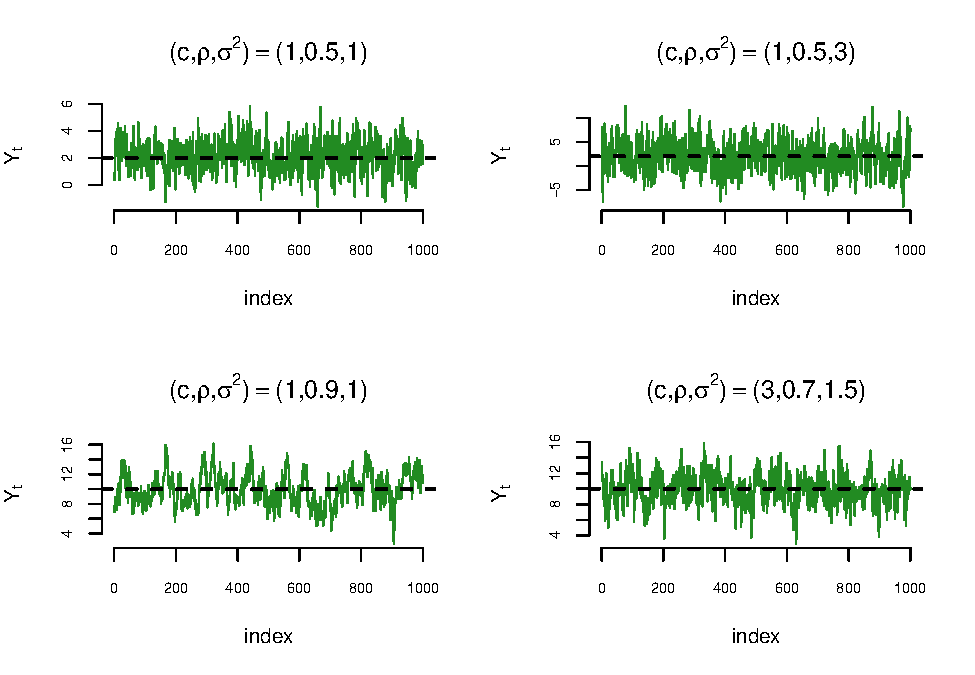
\includegraphics[width=0.8\linewidth]{Sem_1_files/figure-latex/unnamed-chunk-19-1} \end{center}

Considerăm setul de parametrii \((c, \rho, \sigma^2) = (1, 0.5, 1)\) și
calculăm estimatorul de verosimilitate maximă plecând de la logaritmul
funcției de verosimilitate (utilizăm funcția \texttt{optim()}):

\begin{Shaded}
\begin{Highlighting}[]
\NormalTok{y =}\StringTok{ }\KeywordTok{genAR1}\NormalTok{(}\DecValTok{1000}\NormalTok{, }\DecValTok{1}\NormalTok{, }\FloatTok{0.5}\NormalTok{, }\DecValTok{1}\NormalTok{)}
  
\NormalTok{loglik_AR1 =}\StringTok{ }\ControlFlowTok{function}\NormalTok{(param)\{}
  \CommentTok{# pentru a folosi functia optim trebuie sa avem un singur argument}
  \CommentTok{# parametrii}
\NormalTok{  c =}\StringTok{ }\NormalTok{param[}\DecValTok{1}\NormalTok{]}
\NormalTok{  rho =}\StringTok{ }\NormalTok{param[}\DecValTok{2}\NormalTok{]}
\NormalTok{  sigma =}\StringTok{ }\NormalTok{param[}\DecValTok{3}\NormalTok{]}
  
  \CommentTok{# esantionul}
\NormalTok{  ly =}\StringTok{ }\KeywordTok{length}\NormalTok{(y) }\CommentTok{# talia esantionului}
  
  \CommentTok{# prima observatie}
\NormalTok{  l1 =}\StringTok{ }\KeywordTok{log}\NormalTok{(}\KeywordTok{dnorm}\NormalTok{(y[}\DecValTok{1}\NormalTok{], }\DataTypeTok{mean =}\NormalTok{ c}\OperatorTok{/}\NormalTok{(}\DecValTok{1}\OperatorTok{-}\NormalTok{rho), }\DataTypeTok{sd =} \KeywordTok{sqrt}\NormalTok{(sigma}\OperatorTok{^}\DecValTok{2}\OperatorTok{/}\NormalTok{(}\DecValTok{1}\OperatorTok{-}\NormalTok{rho}\OperatorTok{^}\DecValTok{2}\NormalTok{))))}
  
  \CommentTok{# celelalte observatii}
\NormalTok{  dif =}\StringTok{ }\NormalTok{y[}\DecValTok{2}\OperatorTok{:}\NormalTok{ly] }\OperatorTok{-}\StringTok{ }\NormalTok{c }\OperatorTok{-}\StringTok{ }\NormalTok{rho}\OperatorTok{*}\NormalTok{y[}\DecValTok{1}\OperatorTok{:}\NormalTok{(ly}\OperatorTok{-}\DecValTok{1}\NormalTok{)]}
\NormalTok{  l2 =}\StringTok{ }\KeywordTok{log}\NormalTok{(}\KeywordTok{dnorm}\NormalTok{(dif, }\DecValTok{0}\NormalTok{, sigma))}
  
  \CommentTok{# logaritmul verosimilitatii}
\NormalTok{  l =}\StringTok{ }\NormalTok{l1 }\OperatorTok{+}\StringTok{ }\KeywordTok{sum}\NormalTok{(l2)}
  
  \CommentTok{# intoarcem -l pentru ca vrem maximul}
  \KeywordTok{return}\NormalTok{(}\OperatorTok{-}\NormalTok{l)}
\NormalTok{\}}
 
\CommentTok{# determinam MLE }
\NormalTok{param =}\StringTok{ }\KeywordTok{c}\NormalTok{(}\FloatTok{0.6}\NormalTok{, }\FloatTok{0.6}\NormalTok{, }\FloatTok{0.6}\NormalTok{)}
\NormalTok{MLE =}\StringTok{ }\KeywordTok{optim}\NormalTok{(param, loglik_AR1)}\OperatorTok{$}\NormalTok{par}
\end{Highlighting}
\end{Shaded}

Obținem următoarele rezultate

\rowcolors{2}{gray!6}{white}

\begin{longtable}{lrr}
\hiderowcolors
\toprule
  & Theta & MLE\\
\midrule
\endfirsthead
\multicolumn{3}{@{}l}{\textit{(continued)}}\\
\toprule
  & Theta & MLE\\
\midrule
\endhead
\
\endfoot
\bottomrule
\endlastfoot
\showrowcolors
c & 1.0 & 0.9261046\\
rho & 0.5 & 0.5211693\\
sigma & 1.0 & 1.0104216\\*
\end{longtable}

\rowcolors{2}{white}{white}

care sunt apropiate de valorile reale.

\begin{rmdexercise}
\marginnote{\enonce{13006}{}}\vspace{-7mm}

Acum considerăm că prima observație \(y_1\) este dată (deterministă) și
avem \(f_{Y_1}(y_1;\boldsymbol{\theta})\). Scrieți logaritmul funcției
de verosimilitate a modelului \(AR(1)\) pentru eșantionul
\(y_1,y_2,\ldots,y_T\).
\end{rmdexercise}

Funcția de verosimilitate condiționată este definită prin

\[
  L(\boldsymbol{\theta};y_2,\ldots, y_T|y_1) = \prod_{t = 2}^{T}f_{Y_t|Y_{t-1}, Y_1 = y_1}(y_t|y_{t-1}, y_1;\boldsymbol{\theta})\times \underbrace{f_{Y_1}(y_1;\boldsymbol{\theta})}_{ = 1} = \prod_{t = 2}^{T}f_{Y_t|Y_{t-1}}(y_t|y_{t-1};\boldsymbol{\theta})
\]

iar logaritmul funcției de verosimilitate condiționtă devine

\[
  l(\boldsymbol{\theta};y_2,\ldots, y_T|y_1) = \sum_{t = 2}^{T}l_t(\boldsymbol{\theta};y_t|y_{t-1})
\]

cu
\(l_t(\boldsymbol{\theta};y_t|y_{t-1}) = \log(f_{Y_t|Y_{t-1}}(y_t|y_{t-1};\boldsymbol{\theta}))\).
Găsim că

\[
  l(\boldsymbol{\theta};y_2,\ldots, y_T|y_1) = -\frac{T-1}{2}\log(2\pi\sigma^2) - \frac{1}{2\sigma^2}\sum_{t = 2}^{T}(y_t - c - \rho y_{t-1})^2.
\]

\section{Testarea ipotezelor
statistice}\label{testarea-ipotezelor-statistice}

\subsection{Teste parametrice și Lema
Neyman-Pearson}\label{teste-parametrice-si-lema-neyman-pearson}

Să presupunem că ne aflăm în contextul următoarei probleme:

\begin{rmdexercise}
\marginnote{\enonce{21001}{}}\vspace{-7mm}

Fie \(U\) și \(V\) două variablie aleatoare independente și repartizate
\(\mathcal{N}(0, \theta)\). Variabila aleatoare \(X\) definită prin

\[
    X = \sqrt{U^2 + V^2}
\]

este repartizată \emph{Rayleigh} de parametru \(\theta\),
\(X\sim \text{Rayleigh}(\theta)\), și are densitatea

\[
  f_{\theta}(x) = \frac{x}{\theta}e^{-\frac{x^2}{2\theta}},\quad \forall x\in[0,\infty]
\]
\end{rmdexercise}

Pentru mai multe detalii privind repartiția Rayleigh se poate consulta
pagina \url{https://en.wikipedia.org/wiki/Rayleigh_distribution} sau
monografia \citep{Evans2000}. Densitatea de repartiție și funcția de
repartiție a repartiției Rayleigh sunt ilustrate mai jos (pentru a
folosi în R funcțiile: \texttt{rrayleigh}, \texttt{drayleigh},
\texttt{prayleigh} și respectiv \texttt{qrayleigh} trebuie instalat
pachetul \texttt{VGAM}):

\begin{center}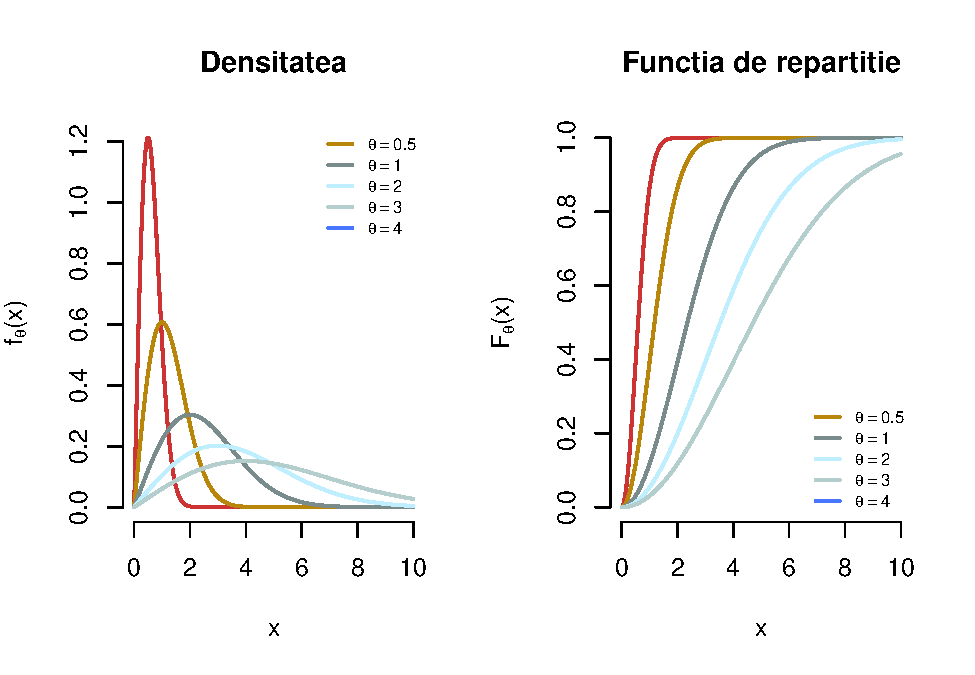
\includegraphics[width=0.8\linewidth]{Sem_1_files/figure-latex/unnamed-chunk-24-1} \end{center}

În cele ce urmează, ne propunem să răspundem la o serie de întrebări:

\begin{rmdexercise}
\marginnote{\enonce{21002}{}}\vspace{-7mm}

Fie \(X_1, X_2, \ldots, X_n\) un eșantion de talie \(n\) dintr-o
populație Rayleigh de parametru \(\theta\). Determinați estimatorul de
verosimilitate maximă pentru \(\theta\).
\end{rmdexercise}

Logaritmul funcției de verosimilitate este dat de

\[
  l(\theta|\mathbf{x}) = \sum_{i=1}^{n}\log{f_{\theta}(x_i)} = \sum_{i = 1}^{n}\log(x_i) - n\log(\theta) + \frac{1}{2\theta}\sum_{i = 1}^{n}x_i^2
\]

iar estimatorul de verosimilitate verifică

\[
  \hat{\theta}_n = \underset{\theta>0}{\arg\max}\, l(\theta|\mathbf{x}) = \underset{\theta>0}{\arg\max}\, \sum_{i = 1}^{n}\log(x_i) - n\log(\theta) + \frac{1}{2\theta}\sum_{i = 1}^{n}x_i^2.
\]

Rezolvând ecuația de verosimilitatea (condiția de ordin 1)

\[
  \left. \frac{\partial l(\theta|\mathbf{x})}{\partial\theta}\right\vert_{\hat{\theta}_n} = -\frac{n}{\hat{\theta}_n} + \frac{1}{2\hat{\theta}_n^2}\sum_{i = 1}^{n}x_i^2 = 0
\]

găsim că

\[
  \hat{\theta}_n = \frac{1}{2n}\sum_{i = 1}^{n} X_i^2.
\]

Pentru a vedea că într-adevăr \(\hat{\theta}_n\) este estimatorul de
verosimilitate maximă trebuie să verificăm condiția de ordin 2

\[
  \left. \frac{\partial^2 l(\theta|\mathbf{x})}{\partial\theta^2}\right\vert_{\hat{\theta}_n} = \frac{n}{\hat{\theta}_n^2} - \frac{1}{\hat{\theta}_n^3}\sum_{i = 1}^{n}x_i^2 = \frac{n}{\hat{\theta}_n^2} - \frac{2n\hat{\theta}_n}{\hat{\theta}_n^3} = - \frac{n}{\hat{\theta}_n^2}<0 
\]

unde am folosit faptul că \(\sum_{i = 1}^{n}x_i^2 = 2n\hat{\theta}_n\).
Prin urmare \(\hat{\theta}_n\) este estimatorul de verosimilitate
maximă.

\begin{rmdexercise}
\marginnote{\enonce{21003}{}}\vspace{-7mm}

Determinați repartiția asimptotică a EVM \(\hat{\theta}_n\) a lui
\(\theta\).
\end{rmdexercise}

Știm că dacă \(\hat{\theta}_n\) este estimatorul de verosimilitate
maximă pentru \(\theta\) și \(f_{\theta}(x)\) verifică o serie de
condiții de regularitatea atunci are loc

\[
  \sqrt{n}\left(\hat{\theta}_n - \theta_0\right) \underset{n\to\infty}{\overset{d}{\longrightarrow}} \mathcal{N}(0,I_1^{-1}(\theta_0))
\]

unde \(\theta_0\) este valoarea adevărată a parametrului iar
\(I_1^{-1}(\theta_0)\) este informația lui Fisher pentru o observație.
În cazul problemei noastre, informația lui Fisher este

\[
  I_n(\theta) = \mathbb{E}_{\theta}\left[-\frac{\partial^2 \log f_{\theta}(\mathbf{X})}{\partial\theta^2}\right] = \mathbb{E}_{\theta}\left[-\frac{n}{\theta^2} + \frac{1}{\theta^3}\sum_{i = 1}^{n}X_i^2\right] = -\frac{n}{\theta^2} + \frac{1}{\theta^2}\sum_{i = 1}^{n}\mathbb{E}_{\theta}\left[\frac{X_i^2}{\theta}\right]
\]

Cum \(\frac{X^2}{\theta} = \frac{U^2}{\theta} + \frac{V^2}{\theta}\) iar
\(\frac{U}{\sqrt{\theta}}\) și \(\frac{V}{\sqrt{\theta}}\) sunt
variabile aleatoare independente repartizate \(\mathcal{N}(0,1)\)
deducem că \(\frac{X^2}{\theta}\) este repartizată \(\chi^2(2)\) prin
urmare

\[
  \mathbb{E}_{\theta}\left[\frac{X_i^2}{\theta}\right] = 2.
\]

Astfel
\(I_n(\theta) = -\frac{n}{\theta^2} + \frac{2n}{\theta^2} = \frac{n}{\theta^2}\)
de unde \(I_1(\theta) = \frac{n1}{\theta^2}\). Avem

\[
  \sqrt{n}\left(\hat{\theta}_n - \theta\right) \underset{n\to\infty}{\overset{d}{\longrightarrow}} \mathcal{N}(0,I_1^{-1}(\theta)) 
\]

sau echivalent

\[
  \sqrt{n}\left(\hat{\theta}_n - \theta\right) \underset{n\to\infty}{\overset{d}{\longrightarrow}} \mathcal{N}(0,\theta^2). 
\]

\begin{rmdexercise}
\marginnote{\enonce{21004}{}}\vspace{-7mm}

Considerăm testul pentru ipotezele

\[
  H_0:\, \theta = \theta_0 \quad \text{vs}\quad H_1:\, \theta = \theta_1
\]

unde \(\theta_1>\theta_0\). Determinați regiunea critică pentru UMP test
de mărime \(\alpha\) pentru ipotezele \(H_0\) și \(H_1\).
\end{rmdexercise}

Din lema Neyman-Pearson avem că regiunea critică a testului UMP este
dată de

\[
  C = \left\{(x_1,x_2,\ldots,x_n)\,|\,\frac{L_{\theta_0}(x_1,x_2,\ldots,x_n)}{L_{\theta_1}(x_1,x_2,\ldots,x_n)}<k\right\}
\]

unde constatnta \(k\) se determină din mărimea testului \(\alpha\)

\[
  \mathbb{P}_{H_0}((x_1,x_2,\ldots,x_n)\in C) = \alpha.
\]

Prin logaritmare avem

\begin{align*}
   & l(\theta_0|\mathbf{x}) -  l(\theta_1|\mathbf{x}) < \log(k)\\
   \iff & n\left(\log(\theta_1) - \log(\theta_0)\right) + \frac{1}{2}\left(\frac{1}{\theta_1} - \frac{1}{\theta_0}\right)\sum_{i = 1}^{n}x_i^2 < \log(k)\\
   \iff & \frac{1}{2}\left(\frac{1}{\theta_1} - \frac{1}{\theta_0}\right)\sum_{i = 1}^{n}x_i^2 < k_1 = \log(k) - n\left(\log(\theta_1) - \log(\theta_0)\right)
\end{align*}

sau echivalent, ținând cont de faptul că \(\theta_1>\theta_0\), avem

\[
  \frac{1}{2n}\sum_{i = 1}^{n}x_i^2 > c
\]

unde \(c = \frac{k_1 \theta_0 \theta_1}{n(\theta_0 - \theta_1)}\).

Regiunea critică pentru testul UMP de mărime \(\alpha\) cu ipotezele

\[
  H_0:\, \theta = \theta_0 \quad \text{vs}\quad H_1:\, \theta = \theta_1
\]

unde \(\theta_1>\theta_0\) este

\[
  C = \left\{(x_1,x_2,\ldots,x_n)\,|\,\hat{\theta}_n = \frac{1}{2n}\sum_{i = 1}^{n}x_i^2 > c\right\}.
\]

Constanta \(c\) se determină din condiția

\[
  \alpha = \mathbb{P}_{H_0}(C) = \mathbb{P}_{H_0}(\hat{\theta}_n > c).
\] Sub ipoteza nulă, dacă \(n\) este suficient de mare, am văzut că

\[
  \hat{\theta}_n \underset{H_0}{\approx} \mathcal{N}\left(\theta_0, \frac{\theta_0^2}{n}\right)
\]

prin urmare

\[
  1-\alpha = \mathbb{P}_{H_0}\left(\sqrt{n}\frac{\hat{\theta}_n - \theta_0}{\theta_0}<\sqrt{n}\frac{c - \theta_0}{\theta_0}\right)
\]

de unde \(c = \theta_0 + \frac{\theta_0}{\sqrt{n}}z_{1-\alpha}\) cu
\(z_{1-\alpha} = \Phi^{-1}(1-\alpha)\).

Regiunea critică a testului UMP cu ipotezele \(H_0\,\,vs\,\,H_1\) devine

\[
  C = \left\{\mathbf{x}\,|\,\hat{\theta}_n(\mathbf{x}) > \theta_0 + \frac{\theta_0}{\sqrt{n}}z_{1-\alpha}\right\}.
\]

\begin{rmdexercise}
\marginnote{\enonce{21005}{}}\vspace{-7mm}

Considerăm testul pentru ipotezele

\[
  H_0:\, \theta = 2 \quad \text{vs}\quad H_1:\, \theta > 2
\]

Știind că pentru un eșantion de talie \(n = 100\) avem
\(\sum_{i = 1}^{n}x_i^2 = 470\) care este concluzia testului pentru un
prag de semnificație de \(10\%\)?
\end{rmdexercise}

Considerăm testul cu ipotezele

\[
  H_0:\, \theta = \theta_0 \quad \text{vs}\quad H_1:\, \theta = \theta_1
\]

unde \(\theta_1>\theta_0\). Am văzut că regiunea critică a testului UMP
de mărime \(\alpha\) este

\[
  C = \left\{\mathbf{x}\,|\,\hat{\theta}_n(\mathbf{x}) > \theta_0 + \frac{\theta_0}{\sqrt{n}}z_{1-\alpha}\right\}.
\]

Cum regiunea critică nu depinde de \(\theta_1\) (în plus raportul de
verosimilitate verifică proprietatea de monotonie), ea corespunde și la
testul unilateral UMP de mărime \(\alpha\):

\[
  H_0:\, \theta = \theta_0 \quad \text{vs}\quad H_1:\, \theta > \theta_0
\]

Pentru \(\theta_0 = 2\), \(n = 100\) și \(\alpha = 0.1\) obținem

\[
  C = \left\{\mathbf{x}\,|\,\hat{\theta}_n(\mathbf{x}) > 2 + \frac{2}{10}z_{0.9}\right\} = \left\{\mathbf{x}\,|\,\hat{\theta}_n(\mathbf{x}) > 2.2563\right\}
\]

Cum, din ipoteză avem că \(\sum_{i = 1}^{n}x_i^2 = 470\), pentru
\(n = 100\) deducem că

\[
  \hat{\theta}_n(\mathbf{x}) = \frac{1}{2n}\sum_{i = 1}^{n}x_i^2 = \frac{470}{200} = 2.35
\]

ceea ce arată că pentru pragul de semnificație de \(\alpha = 10\%\)
respingem ipoteza nulă \(H_0:\, \theta = 2\).

\begin{rmdexercise}
\marginnote{\enonce{21006}{}}\vspace{-7mm}

Determinați puterea testului unilateral UMP de mărime \(\alpha\) pentru
ipotezele

\[
   H_0:\, \theta = \theta_0 \quad \text{vs}\quad H_1:\, \theta > \theta_0
\]

Ilustrați grafic în R pentru \(n = 100\), \(\theta_0 = 2\) și
\(\alpha = 0.1\).
\end{rmdexercise}

Am văzut că regiunea critică este dată de

\[
 C = \left\{\mathbf{x}\,|\,\hat{\theta}_n(\mathbf{x}) > \theta_0 + \frac{\theta_0}{\sqrt{n}}z_{1-\alpha}\right\}
\]

iar din definiția funcției putere avem că

\[
 pow(\theta) = \mathbb{P}_{H_1}(\mathbf{x}\in C) = \mathbb{P}_{H_1}(\hat{\theta}_n(\mathbf{x}) > a)
\]

cu \(a = \theta_0 + \frac{\theta_0}{\sqrt{n}}z_{1-\alpha}\).

Sub ipoteza alternativă avem că

\[
  \hat{\theta}_n \underset{H_1}{\approx} \mathcal{N}\left(\theta, \frac{\theta^2}{n}\right),\quad \theta>\theta_0
\]

prin urmare puterea este

\[
  pow(\theta) = 1 - \mathbb{P}_{H_1}\left(\sqrt{n}\frac{\hat{\theta}_n - \theta}{\theta}<\sqrt{n}\frac{a - \theta}{\theta}\right) = 1 - \Phi\left(\sqrt{n}\frac{a - \theta}{\theta}\right) = 1 - \Phi\left(\sqrt{n}\frac{\theta_0 - \theta}{\theta} + \frac{\theta_0}{\theta}z_{1-\alpha}\right),\, \theta>\theta_0.
\]

Particularizând, pentru \(\theta_0 = 2\), \(n = 100\) și
\(\alpha = 0.1\) obținem

\[
  pow(\theta) = 1 - \Phi\left(10\frac{2 - \theta}{\theta} + \frac{2.5631}{\theta}\right),\, \theta>2.
\]

Ilustrăm în R funcția putere a testului pentru ipotezele
\(H_0:\, \theta = \theta_0 \quad \text{vs}\quad H_1:\, \theta > \theta_0\):

\begin{Shaded}
\begin{Highlighting}[]
\NormalTok{pow_graf =}\StringTok{ }\ControlFlowTok{function}\NormalTok{(theta, theta0, alpha, n)\{}
\NormalTok{  z =}\StringTok{ }\KeywordTok{qnorm}\NormalTok{(}\DecValTok{1}\OperatorTok{-}\NormalTok{alpha)}
\NormalTok{  pow =}\StringTok{ }\DecValTok{1} \OperatorTok{-}\StringTok{ }\KeywordTok{pnorm}\NormalTok{(}\KeywordTok{sqrt}\NormalTok{(n)}\OperatorTok{*}\NormalTok{(theta0 }\OperatorTok{-}\StringTok{ }\NormalTok{theta)}\OperatorTok{/}\NormalTok{theta }\OperatorTok{+}\StringTok{ }\NormalTok{theta0}\OperatorTok{/}\NormalTok{theta}\OperatorTok{*}\NormalTok{z)}
  
  \KeywordTok{return}\NormalTok{(pow)}
\NormalTok{\}}
\end{Highlighting}
\end{Shaded}

\begin{center}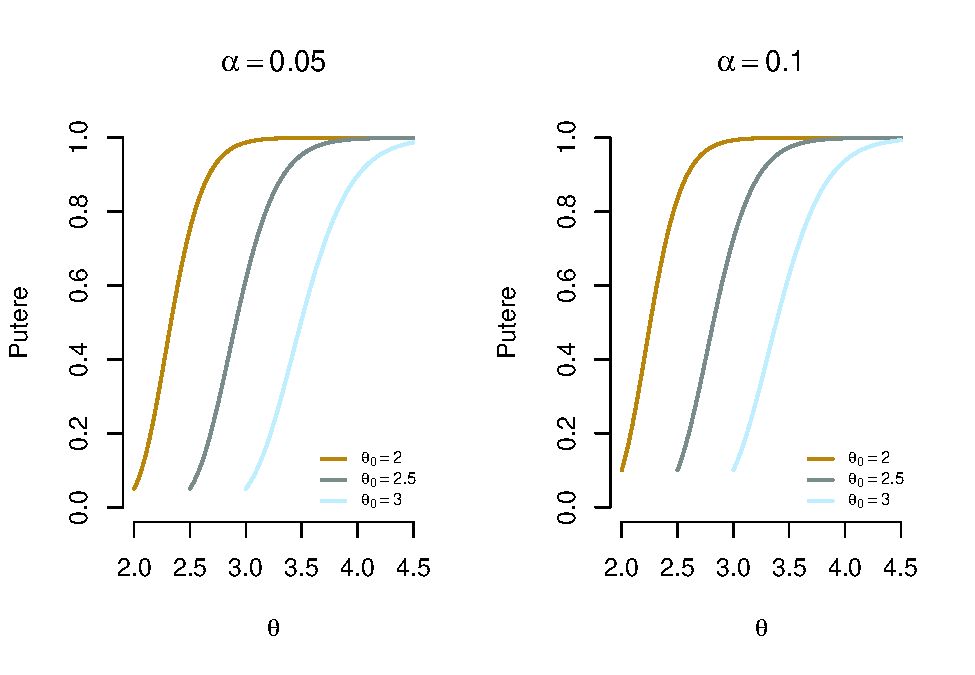
\includegraphics[width=0.8\linewidth]{Sem_1_files/figure-latex/unnamed-chunk-31-1} \end{center}

\begin{rmdexercise}
\marginnote{\enonce{21007}{}}\vspace{-7mm}

Considerăm testul bilateral pentru ipotezele

\[
  H_0:\, \theta = \theta_0 \quad \text{vs}\quad H_1:\, \theta \neq \theta_0
\]

Care este regiunea critică a testului de mărime \(\alpha\)?
\end{rmdexercise}

Considerăm testele unilaterale

\[
\begin{array}{ll}
  \text{Testul A} & H_0:\, \theta = \theta_0 \quad \text{vs}\quad H_1:\, \theta < \theta_0\\
  \text{Testul B} & H_0:\, \theta = \theta_0 \quad \text{vs}\quad H_1:\, \theta > \theta_0\\
\end{array}
\]

Regiunile critice ale celor două teste unilaterale UMP de mărime
\(\frac{\alpha}{2}\) sunt, după cum am văzut la întrebările precedente,
date de

\begin{align*}
  C_A &= \left\{\mathbf{x}\,|\,\hat{\theta}_n(\mathbf{x}) < \theta_0 + \frac{\theta_0}{\sqrt{n}}z_{\frac{\alpha}{2}}\right\}\\
  C_B &= \left\{\mathbf{x}\,|\,\hat{\theta}_n(\mathbf{x}) > \theta_0 + \frac{\theta_0}{\sqrt{n}}z_{1-\frac{\alpha}{2}}\right\}
\end{align*}

iar regiunea critică a testului bilateral este dată de reuniunea
acestora

\[
  C = C_A\cup C_B = \left\{\mathbf{x}\,|\,\hat{\theta}_n(\mathbf{x}) < \theta_0 + \frac{\theta_0}{\sqrt{n}}z_{\frac{\alpha}{2}}\right\} \bigcup \left\{\mathbf{x}\,|\,\hat{\theta}_n(\mathbf{x}) > \theta_0 + \frac{\theta_0}{\sqrt{n}}z_{1-\frac{\alpha}{2}}\right\}.
\]

Știind că \(z_{\frac{\alpha}{2}} = -z_{1-\frac{\alpha}{2}}\) această
regiune critică se poate scrie sub forma

\[
  C = \left\{\mathbf{x}\,|\,\left|\hat{\theta}_n(\mathbf{x}) - \theta_0\right| > \frac{\theta_0}{\sqrt{n}}z_{1-\frac{\alpha}{2}}\right\}.
\]

\begin{rmdexercise}
\marginnote{\enonce{21008}{}}\vspace{-7mm}

Determinați puterea testului bilateral de mărime \(\alpha\) pentru
ipotezele

\[
   H_0:\, \theta = \theta_0 \quad \text{vs}\quad H_1:\, \theta \neq \theta_0
\]

Ilustrați grafic în R pentru \(n = 100\), \(\theta_0 = 2\) și
\(\alpha = 0.1\).
\end{rmdexercise}

Pentru a determina puterea testului avem, conform definiției, că

\[
   pow(\theta) = \mathbb{P}_{H_1}(\mathbf{x}\in C) = 1 - \mathbb{P}_{H_1}(\mathbf{x}\in C^c).
\]

Regiunea de acceptare \(C^c\) este dată de

\[
  C^c = \left\{\mathbf{x}\,|\, \theta_0 - \frac{\theta_0}{\sqrt{n}}z_{1-\frac{\alpha}{2}}<\hat{\theta}_n(\mathbf{x}) < \theta_0 + \frac{\theta_0}{\sqrt{n}}z_{1-\frac{\alpha}{2}}\right\}
\]

de unde funcția putere devine

\[
  pow(\theta) = 1 - \mathbb{P}_{H_1}\left(\hat{\theta}_n(\mathbf{x}) < \theta_0 + \frac{\theta_0}{\sqrt{n}}z_{1-\frac{\alpha}{2}}\right) + \mathbb{P}_{H_1}\left(\hat{\theta}_n(\mathbf{x}) < \theta_0 - \frac{\theta_0}{\sqrt{n}}z_{1-\frac{\alpha}{2}}\right).
\]

Sub ipoteza alternativă, \(H_1\), am văzut că estimatorul de
verosimilitate maximă \(\hat{\theta}_n(\mathbf{x})\) este repartizat
asimptotic

\[
  \hat{\theta}_n \underset{H_1}{\approx} \mathcal{N}\left(\theta, \frac{\theta^2}{n}\right),\quad \theta \neq \theta_0
\]

prin urmare funcția putere se scrie

\[
  pow(\theta) \approx 1 - \Phi\left(\sqrt{n}\frac{\theta_0 - \theta}{\theta} + \frac{\theta_0}{\theta}z_{1-\frac{\alpha}{2}}\right) + \Phi\left(\sqrt{n}\frac{\theta_0 - \theta}{\theta} - \frac{\theta_0}{\theta}z_{1-\frac{\alpha}{2}}\right),\,\theta\neq \theta_0
\]

Particularizând, pentru \(\theta_0 = 2\), \(n = 100\) și
\(\alpha = 0.1\) obținem

\[
  pow(\theta) = 1 - \Phi\left(10\frac{2 - \theta}{\theta} + \frac{2.5631}{\theta}\right) + \Phi\left(10\frac{2 - \theta}{\theta} - \frac{2.5631}{\theta}\right),\, \theta\neq 2.
\]

Ilustrăm în R funcția putere a testului bilateral pentru ipotezele
\(H_0:\, \theta = \theta_0 \quad \text{vs}\quad H_1:\, \theta \neq \theta_0\):

\begin{Shaded}
\begin{Highlighting}[]
\NormalTok{pow_graf_bilateral =}\StringTok{ }\ControlFlowTok{function}\NormalTok{(theta, theta0, alpha, n)\{}
\NormalTok{  z =}\StringTok{ }\KeywordTok{qnorm}\NormalTok{(}\DecValTok{1}\OperatorTok{-}\NormalTok{alpha}\OperatorTok{/}\DecValTok{2}\NormalTok{)}
\NormalTok{  pow =}\StringTok{ }\DecValTok{1} \OperatorTok{-}\StringTok{ }\KeywordTok{pnorm}\NormalTok{(}\KeywordTok{sqrt}\NormalTok{(n)}\OperatorTok{*}\NormalTok{(theta0 }\OperatorTok{-}\StringTok{ }\NormalTok{theta)}\OperatorTok{/}\NormalTok{theta }\OperatorTok{+}\StringTok{ }\NormalTok{theta0}\OperatorTok{/}\NormalTok{theta}\OperatorTok{*}\NormalTok{z) }\OperatorTok{+}
\StringTok{    }\KeywordTok{pnorm}\NormalTok{(}\KeywordTok{sqrt}\NormalTok{(n)}\OperatorTok{*}\NormalTok{(theta0 }\OperatorTok{-}\StringTok{ }\NormalTok{theta)}\OperatorTok{/}\NormalTok{theta }\OperatorTok{-}\StringTok{ }\NormalTok{theta0}\OperatorTok{/}\NormalTok{theta}\OperatorTok{*}\NormalTok{z)}
  
  \KeywordTok{return}\NormalTok{(pow)}
\NormalTok{\}}
\end{Highlighting}
\end{Shaded}

\begin{center}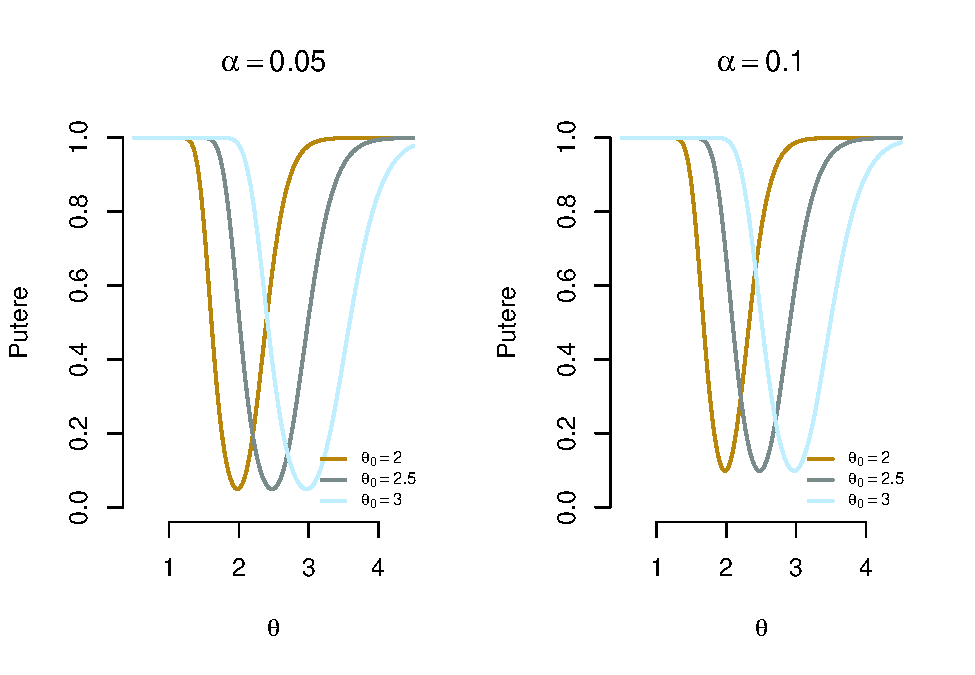
\includegraphics[width=0.8\linewidth]{Sem_1_files/figure-latex/unnamed-chunk-35-1} \end{center}

\begin{rmdexercise}
\marginnote{\enonce{21009}{}}\vspace{-7mm}

Arătați că testul bilateral este nedeplasat și consistent.
\end{rmdexercise}

Am văzut că puterea testului bilateral este dată de

\[
  pow(\theta) \approx 1 - \Phi\left(\sqrt{n}\frac{\theta_0 - \theta}{\theta} + \frac{\theta_0}{\theta}z_{1-\frac{\alpha}{2}}\right) + \Phi\left(\sqrt{n}\frac{\theta_0 - \theta}{\theta} - \frac{\theta_0}{\theta}z_{1-\frac{\alpha}{2}}\right),\,\theta\neq \theta_0
\]

Pentru \(\theta<\theta_0\) obținem

\[
 \lim_{n\to\infty}pow(\theta) = 1 - \Phi(\infty) + \Phi(\infty) = 1 - 1 + 1 = 1
\]

iar pentru \(\theta>\theta_0\)

\[
 \lim_{n\to\infty}pow(\theta) = 1 - \Phi(-\infty) + \Phi(-\infty) = 1 - 0 + 0 = 1
\]

deci testul este consistent.

Pentru a vedea dacă testul este nedeplasat trebuie să calculăm minimul
funcției putere. Se poate observa că acest minim se atinge pentru
\(\theta\to \theta_0\), și cum

\[
  \lim_{\theta\to\theta_0} pow(\theta) = 1 - \Phi\left(z_{1-\frac{\alpha}{2}}\right) + \Phi\left(-z_{1-\frac{\alpha}{2}}\right) = 1 - \left(1-\frac{\alpha}{2}\right) + \frac{\alpha}{2} = \alpha
\]

deducem că testul este nedeplasat.

\subsection{Test bazat pe raportul de
verosimilități}\label{test-bazat-pe-raportul-de-verosimilitati}

Presupunem că \(Y\) este o variabilă aleatoare care ia valori în
mulțimea \(\{y_1,y_2,\ldots,y_c\}\) iar repartiția ei este dată de

\[
\mathbb{P}\circ Y^{-1} = \sum_{j = 1}^{c}p_j\delta_{y_j},
\]

unde \(\mathbb{P}(Y = y_j) = p_{j},\, j\in\{1,2,\ldots,c\}\).

Fie \(Y_1, Y_2,\ldots, Y_n\) un eșantion de talie \(n\) din populația
\(\mathbb{P}\circ Y^{-1}\) și

\[
  N_i = \sum_{k = 1}^{n}\mathbf{1}_{y_i}(Y_k)
\]

numărul de observații care categoria \(y_i\). Observăm că variabilele
aleatoare \(N_1, N_2, \ldots, N_c\) verifică

\[
  N_1 + N_2 +\cdots+ N_c = n.
\]

Putem modela o observație \(Y_k\) dintr-o variabilă discretă cu \(c\)
categorii cu ajutorul unui vector elemente de \(\{0,1\}\),
\((X_1^{(k)}, X_2^{(k)}, \ldots, X_c^{(k)})\), pentru care componenta
\(j\) ia valoarea \(1\) dacă \(Y_k = y_j\) și \(0\) altfel. Funcția de
masă a \(c\)-uplului este

\[
\mathbb{P}((X_1^{(k)}, X_2^{(k)}, \ldots, X_c^{(k)}) = (x_1,x_2,\ldots,x_c)) = p_1^{x_1}p_2^{x_2}\cdots p_c^{x_c}
\]

unde \(x_j\in\{0,1\}\) cu \(\sum_{j = 1}^{c}x_j = 1\). Pentru un
eșantion de talie \(n\),
\(\{(X_1^{(k)}, X_2^{(k)}, \ldots, X_c^{(k)}),\, k = 1,2,\ldots, n\}\)
avem

\[
\mathbb{P}\left((X_1^{(k)}, X_2^{(k)}, \ldots, X_c^{(k)}) = (x_1^{(k)},x_2^{(k)},\ldots,x_c^{(k)}), \,k = 1,2,\ldots,n\right) = \prod_{k=1}^{n}p_1^{x_1^{(k)}}p_2^{x_2^{(k)}}\cdots p_c^{x_c^{(k)}} = p_1^{n_1}p_2^{n_2}\cdots p_c^{n_c}
\]

unde \(n_j\) reprezintă numărul de observații din categoria \(y_j\) iar
\(\sum_{j = 1}^{c}n_j = n\).

În următorul exercițiu ne propunem să aplicăm testul bazat pe raportul
de verosimilități pentru efectuarea unui test asupra parametrilor unei
repartiții multinomiale.

\begin{rmdexercise}
\marginnote{\enonce{22001}{}}\vspace{-7mm}

Spunem că vectorul \((N_1, N_2,\ldots, N_c)\) este repartizat
multinomial \(\mathcal{M}(n;p_1,p_2,\ldots,p_c)\) dacă

\[
  \mathbb{P}(N_1 = n_1, N_2 = n_2, \ldots, N_c = n_c) = \frac{n!}{n_1!n_2!\cdots n_c!}p_1^{n_1}p_2^{n_2}\cdots p_c^{n_c}
\]

unde \(n_1 + n_2 +\cdots+n_c = n\).

Determinați repartiția marginală a lui \(N_i\).
\end{rmdexercise}

Observăm că

\scriptsize

\begin{align*}
  \mathbb{P}(N_i = n_i) &= \sum_{n_1}\cdots\sum_{n_{i-1}}\sum_{n_{i+1}}\cdots\sum_{n_{c}}\mathbb{P}(N_1 = n_1, \ldots, N_{i-1} = n_{i-1}, N_i = n_i, N_{i+1} = n_{i+1}, \ldots, N_c = n_c),  \; n_1 + \cdots + n_c = n - n_i\\
    &= \sum_{n_1}\cdots\sum_{n_{i-1}}\sum_{n_{i+1}}\cdots\sum_{n_{c}}\frac{n!}{n_1!\cdots n_c!}p_1^{n_1}\cdots p_{c}^{n_c},  \; n_1 + \cdots + n_c = n - n_i\\
    &= \frac{n!p_i^{n_i}}{n_i!(n-n_i)!}\sum_{n_1}\cdots\sum_{n_{i-1}}\sum_{n_{i+1}}\cdots\sum_{n_{c}}\frac{(n-n_i)!}{n_1!\cdots n_{i-1}!n_{i+1}!\cdots n_c!}p_1^{n_1}\cdots p_{i-1}^{n_{i-1}}p_{i+1}^{n_{i+1}}\cdots p_{c}^{n_c},  \; n_1 + \cdots + n_c = n - n_i\\
    &= \binom{n}{n_i}p_i^{n_i}(1-p_i)^{n-n_i}\underbrace{\sum_{n_1}\cdots\sum_{n_{i-1}}\sum_{n_{i+1}}\cdots\sum_{n_{c}}\binom{n-n_i}{n_1,\ldots,n_c}\left(\frac{p_1}{1-p_i}\right)^{n_1}\cdots \left(\frac{p_{i-1}}{1-p_i}\right)^{n_{i-1}}\left(\frac{p_{i+1}}{1-p_i}\right)^{n_{i+1}}\cdots \left(\frac{p_c}{1-p_i}\right)^{n_c}}_{=1}\\
    &= \binom{n}{n_i}p_i^{n_i}(1-p_i)^{n-n_i}
\end{align*}

\normalsize

prin urmare \(N\sim\mathcal{B}(n, p_i)\).

\begin{rmdexercise}
\marginnote{\enonce{22002}{}}\vspace{-7mm}

Considerăm ipotezele

\begin{align*}
  H_0: & \{(p_1,p_2,\ldots, p_c) = (\pi_1,\pi_2,\ldots, \pi_c)\}\\
  H_1: & \{\exists i \text{ astfel incat } p_i\neq \pi_i\}
\end{align*}

unde \((\pi_1,\pi_2,\ldots, \pi_c)\) sunt probabilități specificate în
avans. Construiți testul bazat pe raportul de verosimilități
corespunzător.
\end{rmdexercise}

Testul bazat pe raportul de verosimilitate este

\[
  \Lambda(\mathbf{x})=\frac{\sup_{\theta\in\Theta_0}L(\theta|\mathbf{x})}{\sup_{\theta\in\Theta}L(\theta|\mathbf{x})},
\]

unde \(\Theta\) este spațiul parametrilor modelului, \(\Theta_0\) este
spațiul parametrilor corespunzător ipotezei nule iar
\(L(\theta|\mathbf{x})\) este funcția de verosimilitate.

Observăm că spațiul parametrilor corespunzător modelului este

\[
\Theta = \left\{p_1, p_2, \ldots, p_c\,|\,p_{j}\in(0,1),\,\sum_{j = 1}^{c}p_{j} = 1\right\},
\]

cu \(\dim{\Theta} = c-1\), cel corespunzător ipotezei nule este

\[
\Theta_0 = \left\{(p_1,p_2,\ldots, p_c) = (\pi_1,\pi_2,\ldots, \pi_c)\right\}
\]

cu \(\dim{\Theta_0} = 0\) iar funcția de verosimilitate este

\[
  L(p_{j},\,j = 1,\ldots,c\,;\,\mathbf{x}) = \mathbb{P}(N_{j} = n_{j}, \,j = 1,\ldots,c) = \frac{n!}{\prod_{j = 1}^{c} n_{j}!}\prod_{j = 1}^{c} p_{j}^{n_{j}}.
\]

Observăm că

\[
  \sup_{\theta\in\Theta_0}L(\theta|\mathbf{x}) = \mathbb{P}_{H_0}(N_1 = n_1, N_2 = n_2, \ldots, N_c = n_c) = \frac{n!}{\prod_{j = 1}^{c} n_{j}!}\prod_{j = 1}^{c} \pi_{j}^{n_{j}}.
\]

Pentru a determina estimatorul de verosimilitate maximă pe \(\Theta\)
trebuie să rezolvăm problema de optimizare:

\[
  \left\{\begin{array}{ll}
    \max_{\theta\in\Theta} \log L(\theta|\mathbf{x}) = \max \log{\left(\frac{n!}{\prod_{j = 1}^{c} n_{j}!}\prod_{j = 1}^{c} p_{j}^{n_{j}}\right)}\\
    \sum_{j = 1}^{c}p_{j} = 1
  \end{array}\right.
\] Cum logaritmul funcției de verosimilitate este

\[
\log{\left(\frac{n!}{\prod_{j = 1}^{c} n_{j}!}\prod_{j = 1}^{c} p_{j}^{n_{j}}\right)} = \log\left(\frac{n!}{\prod_{j = 1}^{c} n_{j}!}\right) + \sum_{j = 1}^{c}n_{j}\log{p_j}
\]

iar \(p_c = 1 - p_1 -\cdots p_{c-1}\), rezolvând ecuația de
verosimilitate \(\frac{\partial\log{L}}{\partial p_j} = 0\) deducem

\[
\left\{\begin{array}{llll}
  \frac{n_1}{p_1} - \frac{n_c}{1 - p_1 - p_2 -\cdots -p_{c-1}} = 0\\
  \frac{n_2}{p_2} - \frac{n_c}{1 - p_1 - p_2 -\cdots -p_{c-1}} = 0\\
  \cdots\cdots\cdots\cdots\cdots\cdots\cdots\cdots\\
  \frac{n_{c-1}}{p_{c-1}} - \frac{n_c}{1 - p_1 - p_2 -\cdots -p_{c-1}} = 0\\
\end{array}\right.
\]

de unde

\[
  \frac{n_1}{p_1} = \frac{n_2}{p_2} = \cdots = \frac{n_c}{p_c} = \frac{\sum_{j = 1}^{c}n_j}{\sum_{j = 1}^{c}p_j} = n,
\] deci \(\hat{p}_{j} = \frac{n_j}{n}\).

Raportul de verosimilitate devine

\[
\Lambda(\mathbf{x})=\frac{\sup_{\theta\in\Theta_0}L(\theta|\mathbf{x})}{\sup_{\theta\in\Theta}L(\theta|\mathbf{x})} = \frac{\prod_{j = 1}^{c} \pi_{j}^{n_{j}}}{\prod_{j = 1}^{c} \left(\frac{n_{j}}{n}\right)^{n_{j}}} = \prod_{j = 1}^{c}\left(\frac{n\pi_{j}}{n_j}\right)^{n_{j}}
\]

și aplicând
\href{https://en.wikipedia.org/wiki/Likelihood-ratio_test}{Teorema lui
Wilks} găsim

\[
  -2\log \Lambda(\mathbf{x}) = 2\sum_{j = 1}^{c} n_{j}\log\left(\frac{n_{j}}{n\times \pi_{j}}\right) \underset{n\to\infty}{\overset{d}{\longrightarrow}}\chi^2(\underbrace{\dim{\Theta} - \dim{\Theta_0}}_{(c-1)-0}) = \chi^2(c-1).
\]

Prin urmare, regiunea critică a testului asimptotic de nivel \(\alpha\)
bazat pe raportul de verosimilitate este

\[
  C = \left\{\mathbf{x} \,|\, -2\log \Lambda(\mathbf{x}) > \chi^2_{1-\alpha}(c-1)\right\}.
\]

O metodă alternativă este bazată pe statistica \(\chi^2\) a lui Pearson,
\citep{Pearson1900}, care este dată de

\[
  X^2 = \sum_{j = 1}^{c}\frac{(O_{j} - E_{j})^2}{E_{j}}
\]

unde \(O_{j} = n_{j}\) sunt efectivele observate iar \(E_{j}\) sunt
efectivele pe care ne așteptăm să le observăm dacă ipoteza nulă ar fi
adevărată (sub \(H_0\), repartiția condiționată a lui \(N_{j}\) la
\(\sum_{j = 1}^{c}N_{j} = n\) este \(\mathcal{B}(n,p_{j})\)),

\[
  E_{j} = \mathbb{E}_{H_0}[N_{j}] = n \pi_j
\]

ceea ce implică

\[
  X^2 = \sum_{j = 1}^{c}\frac{\left(n_{j} - n \pi_j\right)^2}{n \pi_j}.
\]

Karl Pearson a arătat că această statistică este asimptotic repartizată

\[
  X^2 = \sum_{j = 1}^{c}\frac{\left(n_{j} - n \pi_j\right)^2}{n \pi_j} \underset{n\to\infty}{\overset{d}{\longrightarrow}} \chi^2(c-1)
\]

prin urmare testul \(\chi^2\) a lui Pearson de nivel \(\alpha\), pentru
ipotezele \(H_0\,vs\,H_1\) conduce la aceeași regiune critică ca și
testul bazat pe raportul de verosimilitate (cu toate acestea se poate
arăta că statistica lui Pearson \(X^2\) converge mai repede decât
statistica \(-2\log \Lambda(\mathbf{x})\), \citep{Agresti2012}).

\begin{rmdexercise}
\marginnote{\enonce{22003}{}}\vspace{-7mm}

Un exercițiu constă în extragerea la întâmplare, de către o persoană, a
unei cărți de joc dintr-un pachet amestecat în prealabil, notarea
culorii acesteia (inimă roșie, inimă neagră, romb și treflă) și cărții
în pachet tot aleator. Să presupunem că în urma efectuării exercițiului
pe \(200\) de persoane s-au obținut următoarele rezultate: 35 cărți de
treflă, 51 cărți de romb, 64 cărți de inimă roșie și respectiv 50 cărți
de inimă neagră. Ne propunem să testăm ipotezele

\begin{align*}
  H_0&:\,\{\text{Cele patru culori sunt egal probabile}\}\\
  H_1&:\,\{\text{Cel putin una din cele patru culori este diferita de 0.25}\}
\end{align*}
\end{rmdexercise}

Observăm că dacă notăm cu \(Y\) variabila discretă care ia valori în
mulțimea
\(\{y_1,y_2,y_3,y_4\} = \{\clubsuit, \diamondsuit, \heartsuit, \spadesuit\}\)
și cu \(p_j = \mathbb{P}(Y = y_j)\) atunci ipotezele se scriu

\begin{align*}
  H_0&:\,\{\text{Cele patru culori sunt egal probabile}\} = \{(p_1,p_2,p_3,p_4) = (\pi_1, \pi_2, \pi_3, \pi_4) \,|\, \pi_j = 0.25\}\\
  H_1&:\,\{\text{Cel putin una din cele patru culori este diferita de 0.25}\} = \{\exists j, \text{ astfel ca } p_j\neq 0.25\}
\end{align*}

Avem că tabelul efectivelor observate este

\[
\begin{array}{c|c|c|c}
  \clubsuit & \diamondsuit & \heartsuit & \spadesuit \\
  \hline
  O_1 & O_2 & O_3 & O_4
\end{array} 
=
\begin{array}{c|c|c|c}
  \clubsuit & \diamondsuit & \heartsuit & \spadesuit \\
  \hline
  35 & 51 & 64 & 50
\end{array}
\]

care in R este

\begin{Shaded}
\begin{Highlighting}[]
\NormalTok{tab_observed =}\StringTok{ }\KeywordTok{c}\NormalTok{(}\DecValTok{35}\NormalTok{, }\DecValTok{51}\NormalTok{, }\DecValTok{64}\NormalTok{, }\DecValTok{50}\NormalTok{)}
\end{Highlighting}
\end{Shaded}

iar tabelul efectivelor pe care ne așteptăm să le observăm dacă ipoteza
nulă este adevărată este

\[
\begin{array}{c|c|c|c}
  \clubsuit & \diamondsuit & \heartsuit & \spadesuit \\
  \hline
  E_1 = n\pi_1 & E_2 = n\pi_2 & E_3 = n\pi_3 & E_4 = n\pi_4
\end{array} 
=
\begin{array}{c|c|c|c}
  \clubsuit & \diamondsuit & \heartsuit & \spadesuit \\
  \hline
  50 & 50 & 50 & 50
\end{array}
\]

care în R se scrie

\begin{Shaded}
\begin{Highlighting}[]
\NormalTok{n =}\StringTok{ }\DecValTok{200}
\NormalTok{prob =}\StringTok{ }\KeywordTok{rep}\NormalTok{(}\FloatTok{0.25}\NormalTok{, }\DecValTok{4}\NormalTok{)}

\NormalTok{tab_expected =}\StringTok{ }\NormalTok{n}\OperatorTok{*}\NormalTok{prob}
\end{Highlighting}
\end{Shaded}

Putem calcula acum statistica lui Pearson

\[
  X^2 = \sum_{j = 1}^{c}\frac{(O_{j} - E_{j})^2}{E_{j}} = \sum_{j = 1}^{c}\frac{\left(n_{j} - n \pi_j\right)^2}{n \pi_j}
\]

care devine

\begin{Shaded}
\begin{Highlighting}[]
\NormalTok{alpha =}\StringTok{ }\FloatTok{0.05}
\NormalTok{X2 =}\StringTok{ }\KeywordTok{sum}\NormalTok{((tab_observed }\OperatorTok{-}\StringTok{ }\NormalTok{tab_expected)}\OperatorTok{^}\DecValTok{2}\OperatorTok{/}\NormalTok{tab_expected)}

\CommentTok{# p - valoarea}
\DecValTok{1} \OperatorTok{-}\StringTok{ }\KeywordTok{pchisq}\NormalTok{(X2, }\DataTypeTok{df =} \DecValTok{3}\NormalTok{)}
\NormalTok{[}\DecValTok{1}\NormalTok{] }\FloatTok{0.03774185}
\end{Highlighting}
\end{Shaded}

Acelați rezultat îl obținem și dacă aplicăm funcția
\texttt{chisq.test()}

\begin{Shaded}
\begin{Highlighting}[]
\KeywordTok{chisq.test}\NormalTok{(tab_observed, }\DataTypeTok{p =}\NormalTok{ prob)}

\NormalTok{    Chi}\OperatorTok{-}\NormalTok{squared test }\ControlFlowTok{for}\NormalTok{ given probabilities}

\NormalTok{data}\OperatorTok{:}\StringTok{  }\NormalTok{tab_observed}
\NormalTok{X}\OperatorTok{-}\NormalTok{squared =}\StringTok{ }\FloatTok{8.44}\NormalTok{, df =}\StringTok{ }\DecValTok{3}\NormalTok{, p}\OperatorTok{-}\NormalTok{value =}\StringTok{ }\FloatTok{0.03774}
\end{Highlighting}
\end{Shaded}

Pentru testul bazat pe raportul de verosimilitate maximă avem

\[
  -2\log \Lambda(\mathbf{x}) = -2\sum_{j = 1}^{c} n_{j}\log\left(\frac{n_{j}}{n\times \pi_{j}}\right)
\]

care devine

\begin{Shaded}
\begin{Highlighting}[]
\NormalTok{LRT =}\StringTok{ }\DecValTok{2}\OperatorTok{*}\KeywordTok{sum}\NormalTok{(tab_observed}\OperatorTok{*}\KeywordTok{log}\NormalTok{(tab_observed}\OperatorTok{/}\NormalTok{tab_expected))}

\CommentTok{# p - valoarea}
\DecValTok{1} \OperatorTok{-}\StringTok{ }\KeywordTok{pchisq}\NormalTok{(LRT, }\DataTypeTok{df =} \DecValTok{3}\NormalTok{)}
\NormalTok{[}\DecValTok{1}\NormalTok{] }\FloatTok{0.03431406}
\end{Highlighting}
\end{Shaded}

Ambele proceduri conduc la respingerea ipotezei nule pentru un prag de
semnificație \(\alpha = 0.05\).

\subsection{Testul raportului de verosimilități și testul lui
Wald}\label{testul-raportului-de-verosimilitati-si-testul-lui-wald}

Reamintim că statisticile de test corespunzătoare testului bazat pe
raportul de verosimilități și respectiv pentru testul lui Wald atunci
când testăm ipotezele:

\[
H_0:\, \underbrace{c(\boldsymbol{\theta})}_{p\times 1} = \boldsymbol{0}_{p\times 1} \quad vs\quad H_1:\, c(\boldsymbol{\theta})\neq \boldsymbol{0}_{p\times 1}
\]

unde \(c:\mathbb{R}^k\to\mathbb{R}^p\) este o funcție vectorială

\[
c(\boldsymbol{\theta}) = \begin{pmatrix}c_1(\boldsymbol{\theta}) & c_2(\boldsymbol{\theta}) &\cdots & c_p(\boldsymbol{\theta})\end{pmatrix}^\intercal
\]

cu proprietatea că \(c_i(\boldsymbol{\theta})\) sunt diferențiabile și
nu avem restricții redundante, cu alte cuvinte rangul matricei
\(\frac{\partial c(\boldsymbol{\theta})}{\partial \boldsymbol{\theta}^\intercal}\)
este egal cu \(p\), \(\forall\theta\in\Theta\), sunt date de

\begin{itemize}
\tightlist
\item
  statistica de test pentru testul raportului de verosimilități (Wilks)
\end{itemize}

\[
LRT = -2\log{\Lambda(\mathbf{x})} = -2\log{\frac{\sup_{\theta\in\Theta_0}L(\theta|\mathbf{x})}{\sup_{\theta\in\Theta}L(\theta|\mathbf{x})}} = -2\left(l(\hat{\boldsymbol{\theta}}_{H_0};\mathbf{x}) - l(\hat{\boldsymbol{\theta}};\mathbf{x}) \right)
\]

\begin{itemize}
\tightlist
\item
  statistica de test pentru testul lui Wald
\end{itemize}

\[
W = c(\hat{\boldsymbol{\theta}})^\intercal\left(\frac{\partial c}{\partial \boldsymbol{\theta}^\intercal}(\hat{\boldsymbol{\theta}}) \hat{\mathbb{V}}(\hat{\boldsymbol{\theta}})\frac{\partial c}{\partial \boldsymbol{\theta}^\intercal}(\hat{\boldsymbol{\theta}})^\intercal\right)^{-1}c(\hat{\boldsymbol{\theta}})
\]

unde \(\hat{\mathbb{V}}\) este estimatorul matricei de
varianță-covarianță asimptotică.

Statisticile de test corespunzătoare celor două teste sunt ilustrate
(pentru modelul binomial) în figura de mai jos:

\begin{center}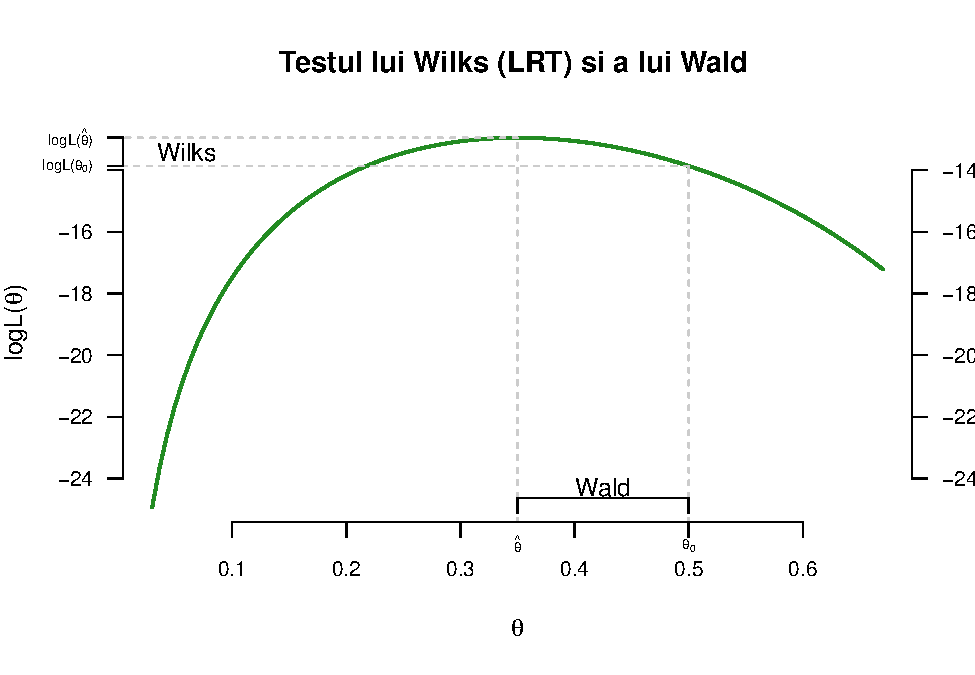
\includegraphics[width=0.8\linewidth]{Sem_1_files/figure-latex/unnamed-chunk-45-1} \end{center}

Exercițiul din această secțiune este preluat din \citep{Greene2011}.

\begin{rmdexercise}
\marginnote{\enonce{23001}{}}\vspace{-7mm}

Considerăm două variabile aleatoare \(X\) și \(Y\) astfel încât
repartiția condiționată a lui \(Y|X = x\) este dată de

\[
  f_{Y|X}(y|x;\beta) = \frac{1}{\beta + x}e^{-\frac{y}{\beta + x}}
\]

Vom nota pentru simplitate cu \(\beta_i = \frac{1}{\beta + x_i}\).
Repartiția condiționată de mai sus este o repartiție exponențială, care
la rândul ei poate fi privită ca un caz particular de repartiție Gamma,
cu \(\rho = 1\),

\[
  f_{Y|X}(y|x;\beta,\rho) = \frac{\beta_i^{\rho}}{\Gamma(\rho)}y^{\rho - 1}e^{-y\beta_i}
\]

Vrem să testăm ipotezele

\[
  H_0:\; \rho = 1 \quad \text{vs}\quad H_1:\; \rho\neq 1
\]
\end{rmdexercise}

Începem prin a reaminti că funcția \(\Gamma(p)\) este definită prin
(vezi și \url{https://en.wikipedia.org/wiki/Gamma_function})

\[
\Gamma(p) = \int_{0}^{\infty}t^{p-1}e^{-t}\,dt,\quad p>0,
\]

verifică relația de recurență

\[
\Gamma(p) = (p-1)\Gamma(p-1)
\]

și \(\Gamma\left(\frac{1}{2}\right) = \sqrt{\pi}\). Mai mult, dacă
\(n\in\mathbb{N}\) atunci \(\Gamma(n+1) = n!\).

De asemenea, derivatele funcției \(\Gamma\) sunt

\[
\frac{d^k \Gamma(p)}{dp^k} = \int_{0}^{\infty}(\log(t))^kt^{p-1}e^{-t}\, dt
\]

iar primele două derivale ale funcției \(\log(\Gamma(p))\), cunoscute și
ca funcțiile
\href{https://en.wikipedia.org/wiki/Digamma_function}{digamma} și
respectiv
\href{https://en.wikipedia.org/wiki/Trigamma_function}{trigamma}, se
notează cu \(\Psi\) și respectiv \(\Psi'\) și sunt definite prin

\begin{align*}
  \Psi &= \frac{\partial \log(\Gamma(p))}{\partial p} = \frac{\Gamma'}{\Gamma}\\
  \Psi' &=\frac{\partial^2 \log(\Gamma(p))}{\partial p^2} = \frac{\Gamma\Gamma'' - \Gamma'^2}{\Gamma^2}
\end{align*}

Aceste funcții sunt implementate în R cu ajutorul funcțiilor
\texttt{digamma()} și respectiv \texttt{trigamma()}.

\begin{center}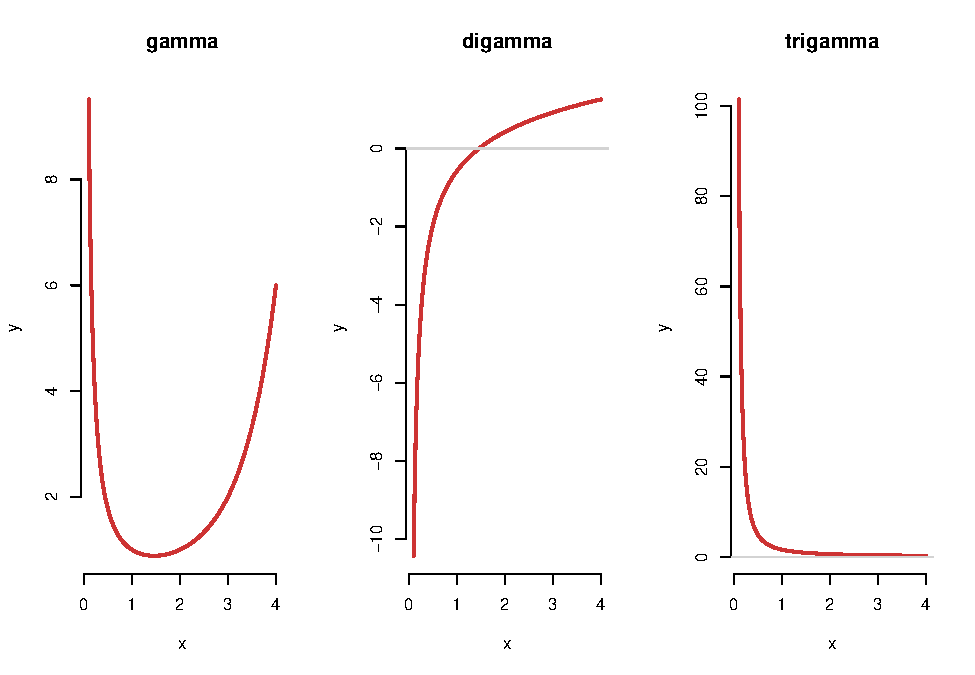
\includegraphics[width=0.8\linewidth]{Sem_1_files/figure-latex/unnamed-chunk-47-1} \end{center}

\begin{rmdexercise}
\marginnote{\enonce{23002}{}}\vspace{-7mm}

Fie \(\{X_i, Y_i\}\) un eșantion de talie \(n\) din populația
\(f_{Y|X}\) și scrieți logaritmul funcției de verosimilitate pentru
modelul necondiționat și respectiv sub \(H_0\) (modelul condiționat).
\end{rmdexercise}

Considerăm parametrul \(\boldsymbol{\theta} = (\beta, \rho)^\intercal\)
și avem

\[
 f_{Y_i|X_i}(y|x;\boldsymbol{\theta}) = \frac{\beta_i^{\rho}}{\Gamma(\rho)}y_i^{\rho - 1}e^{-y_i\beta_i},\quad \text{cu}\quad  \beta_i = \frac{1}{\beta+x_i}
\]

Cum logaritmul funcției de verosimilitate este

\[
  l(y|x;\boldsymbol{\theta}) = \sum_{i = 1}^{n} \log{ f_{Y_i|X_i}(y|x;\boldsymbol{\theta})}
\]

deducem că, sub modelul necondiționat,

\[
  l(y|x;\boldsymbol{\theta}) = \rho\sum_{i = 1}^{n}\beta_i - n\log{\Gamma(\rho)} + (\rho - 1)\sum_{i = 1}^{n}y_i - \sum_{i = 1}^{n}y_i\beta_i.
\]

Sub \(H_0\), \(\rho = 1\) avem

\[
f_{Y_i|X_i}(y|x;\boldsymbol{\theta}) = \beta_i e^{-y_i\beta_i},\quad \text{cu}\quad  \beta_i = \frac{1}{\beta+x_i}
\]

și cum

\[
  l(y|x;\boldsymbol{\theta}) = \sum_{i = 1}^{n} \log{ f_{Y_i|X_i}(y|x;\boldsymbol{\theta})}
\]

găsim că logaritmul funcției de verosimilitate, sub \(H_0\), este

\[
  l(y|x;\boldsymbol{\theta}) = \sum_{i = 1}^{n}\beta_i - \sum_{i = 1}^{n}y_i\beta_i.
\]

\begin{rmdexercise}
\marginnote{\enonce{23003}{}}\vspace{-7mm}

Scrieți vectorii gradient și matricele Hessiene pentru logaritmul
funcției de verosimilitate asociat modelului necondiționat și respectiv
modelului condiționat (sub \(H_0\)).
\end{rmdexercise}

Am văzut la punctul anterior că logaritmul funcției de verosimilitate
pentru modelul necondiționat este

\[
  l(y|x;\boldsymbol{\theta}) = \rho\sum_{i = 1}^{n}\beta_i - n\log{\Gamma(\rho)} + (\rho - 1)\sum_{i = 1}^{n}y_i - \sum_{i = 1}^{n}y_i\beta_i.
\]

Din definiția lui \(\beta_i = \frac{1}{\beta+x_i}\) avem că

\begin{align*}
  \frac{\partial\beta_i}{\partial \beta} &= \frac{\partial\left(\frac{1}{\beta+x_i}\right)}{\partial \beta} = -\frac{1}{(\beta + x_i)^2} = -\beta_i^2\\
  \frac{\partial\log{\beta_i}}{\partial \beta} &= \frac{\partial(-\log{\beta+x_i})}{\partial \beta} = -\frac{1}{\beta + x_i} = -\beta_i
\end{align*}

iar \(\frac{\partial\log{\Gamma(\rho)}}{\partial \rho} = \Psi(\rho)\).

Prin urmare găsim că

\begin{align*}
  \frac{\partial l(y|x;\boldsymbol{\theta})}{\partial \beta} &= -\rho\sum_{i=1}^{n}\beta_i + \sum_{i=1}^{n}y_i\beta_i^2\\
  \frac{\partial l(y|x;\boldsymbol{\theta})}{\partial \rho} &= \sum_{i=1}^{n}\log{\beta_i} - n\Psi(\rho) + \sum_{i=1}^{n}\log{y_i}
\end{align*}

astfel, vectorul gradient sub modelul necondiționat este

\[
\frac{\partial l(y|x;\boldsymbol{\theta})}{\partial \boldsymbol{\theta}} = \begin{pmatrix}
  \frac{\partial l(y|x;\boldsymbol{\theta})}{\partial \beta}\\
  \frac{\partial l(y|x;\boldsymbol{\theta})}{\partial \rho}
\end{pmatrix} = \begin{pmatrix}
  -\rho\sum_{i=1}^{n}\beta_i + \sum_{i=1}^{n}y_i\beta_i^2\\
  \sum_{i=1}^{n}\log{\beta_i} - n\Psi(\rho) + \sum_{i=1}^{n}\log{y_i}
\end{pmatrix}
\]

Pentru matricea Hessiană avem

\[
H(y|x;\boldsymbol{\theta}) = \frac{\partial^2 l(y|x;\boldsymbol{\theta})}{\partial \boldsymbol{\theta}\partial \boldsymbol{\theta}^\intercal} = \begin{pmatrix}
  \frac{\partial^2 l(y|x;\boldsymbol{\theta})}{\partial \beta^2} & \frac{\partial^2 l(y|x;\boldsymbol{\theta})}{\partial \beta\partial \rho}\\
  \frac{\partial^2 l(y|x;\boldsymbol{\theta})}{\partial \rho\partial \beta} & \frac{\partial^2 l(y|x;\boldsymbol{\theta})}{\partial \rho^2}
\end{pmatrix}
\]

și cum

\begin{align*}
  \frac{\partial^2 l(y|x;\boldsymbol{\theta})}{\partial \beta^2} &= \rho\sum_{i=1}^{n}\beta_i^2 - 2\sum_{i=1}^{n}y_i\beta_i^3\\
  \frac{\partial^2 l(y|x;\boldsymbol{\theta})}{\partial \beta\partial \rho} &= \frac{\partial^2 l(y|x;\boldsymbol{\theta})}{\partial \rho\partial \beta} = - \sum_{i=1}^{n}\beta_i\\
  \frac{\partial^2 l(y|x;\boldsymbol{\theta})}{\partial \rho^2} &= -n\Psi'(\rho)
\end{align*}

găsim

\[
H(y|x;\boldsymbol{\theta}) = 
\begin{pmatrix}
  \rho\sum_{i=1}^{n}\beta_i^2 - 2\sum_{i=1}^{n}y_i\beta_i^3 & -\sum_{i=1}^{n}\beta_i \\
  -\sum_{i=1}^{n}\beta_i & -n\Psi'(\rho)
\end{pmatrix}
\]

Sub ipoteza nulă \(H_0\), avem \(\rho = 1\)
(\(\boldsymbol{\theta} = \beta\)) deci vectorul gradient (care acum e
scalar) este

\[
\frac{\partial l(y|x;\boldsymbol{\theta})}{\partial \boldsymbol{\theta}} = \frac{\partial l(y|x;\beta)}{\partial \beta} = -\sum_{i=1}^{n}\beta_i + \sum_{i=1}^{n}y_i\beta_i^2
\]

iar matricea Hessiană (care este tot scalară) este

\[
H(y|x;\boldsymbol{\theta}) = \frac{\partial^2 l(y|x;\beta)}{\partial \beta^2} = \sum_{i=1}^{n}\beta_i^2 - 2\sum_{i=1}^{n}y_i\beta_i^3.
\]

\begin{rmdexercise}
\marginnote{\enonce{23004}{}}\vspace{-7mm}

Scrieți matricea informațională medie a lui Fisher pentru modelul
necondiționat și respectiv modelul condiționat (sub \(H_0\)).
\end{rmdexercise}

Sub modelul necondiționat avem că matricea Hessiană (stocastică) pentru
o observație \(Y_i|x_i\) este

\[
H_i(Y_i|x_i;\boldsymbol{\theta}) = 
  \begin{pmatrix}
    \rho\beta_i^2 - 2Y_i\beta_i^3 & -\beta_i\\ 
    -\beta_i & -\Psi'(\rho)
  \end{pmatrix}
\]

iar matricea informațională medie a lui Fisher pentru o observație se
scrie

\[
  I(\boldsymbol{\theta}) = \mathbb{E}_{X}[I_i(\boldsymbol{\theta})] = \mathbb{E}_{X}[\mathbb{E}_{\boldsymbol{\theta}}[-H_i(Y_i|X_i;\boldsymbol{\theta})]] = \mathbb{E}_{X}\left[\begin{pmatrix}
    -\rho\beta_i^2 + 2\mathbb{E}_{\boldsymbol{\theta}}[Y_i]\beta_i^3 & \beta_i\\ 
    \beta_i & \Psi'(\rho)
  \end{pmatrix}\right]
\]

deoarece \(\beta_i = \frac{1}{\beta+X_i}\) depinde de variabila
aleatoare \(X_i\).

Cum pentru funcția de scor calculată pentru o observație are loc
\(\mathbb{E}_{\boldsymbol{\theta}}[s(Y_i|x_i;\boldsymbol{\theta})] = \mathbf{0}_{2\times 1}\)
deducem că

\[
\mathbb{E}_{\boldsymbol{\theta}}[s(Y_i|x_i;\boldsymbol{\theta})] = \mathbb{E}_{\boldsymbol{\theta}}\left[\begin{pmatrix}
  -\rho\beta_i + Y_i\beta_i^2\\ 
    \log{\beta_i} - \Psi(\rho) + \log{Y_i}
\end{pmatrix}\right] = \mathbf{0}_{2\times 1}
\] de unde
\(\mathbb{E}_{\boldsymbol{\theta}}[Y_i] = \frac{\rho}{\beta_i}\) (media
\(\mathbb{E}_{\boldsymbol{\theta}}\) reprezintă media în raport cu
repartiția condiționată \(Y|X = x\)). Înlocuind în expresia matricei
informaționale medii găsim că

\[
  I(\boldsymbol{\theta}) = \mathbb{E}_{X}\left[\begin{pmatrix}
    \rho\beta_i^2  & \beta_i\\ 
    \beta_i & \Psi'(\rho)
  \end{pmatrix}\right].
\]

Pentru modelul condiționat (sub \(H_0:\rho = 1\),
\(\boldsymbol{\theta} = \beta\)) avem

\begin{align*}
  H_i(Y_i|x_i;\boldsymbol{\theta}) &= H_i(Y_i|x_i;\beta) = \beta_i^2 - 2Y_i\beta_i^3\\
  \mathbb{E}_{\boldsymbol{\theta}}[s(Y_i|x_i;\boldsymbol{\theta})] &= \mathbb{E}_{\beta}[s(Y_i|x_i;\beta)] = \mathbb{E}_{\beta}[-\beta_i + Y_i\beta_i^2] = 0
\end{align*}

ceea ce conduce la \(\mathbb{E}_{\beta}[Y_i] = \frac{1}{\beta_i}\).
Informația medie a lui Fisher pentru o observație sub modelul
condiționat revine la

\[
I(\boldsymbol{\theta}) = I(\beta) = \mathbb{E}_{X}[\mathbb{E}_{\beta}[-H_i(Y_i|X_i;\beta)]] = \mathbb{E}_{X}[-\beta_i^2 + 2\mathbb{E}_{\beta}[Y_i]\beta_i^3] = \mathbb{E}_{X}[\beta_i^2].
\]

\begin{rmdexercise}
\marginnote{\enonce{23005}{}}\vspace{-7mm}

Fie \(\hat{\boldsymbol{\theta}}\) estimatorul de verosimilitate maximă
pentru \(\boldsymbol{\theta} = (\beta, \rho)^\intercal\) pe \(\Theta\)
și \(\hat{\boldsymbol{\theta}}_{H_0}\) estimatorul de verosimilitate
maximă pentru \(\beta\) pe
\(\Theta_0 = \{\boldsymbol{\theta} = (\beta, \rho)^\intercal\,|\,\rho = 1\}\).
Determinați repartițiile asimptotice ale lui
\(\hat{\boldsymbol{\theta}}\) și \(\hat{\boldsymbol{\theta}}_{H_0}\).
\end{rmdexercise}

Am văzut că, atunci când sunt îndeplinite o serie de condiții de
regularitate \citep[Capitolul 14]{Greene2011}, repartiția asimptotică a
lui \(\hat{\boldsymbol{\theta}}\) pentru modelul necondiționat verifică

\[
\sqrt{n}\left(\hat{\boldsymbol{\theta}} - \boldsymbol{\theta}\right) \underset{n\to\infty}{\overset{d}{\longrightarrow}} \mathcal{N}\left(0, I^{-1}(\boldsymbol{\theta})\right)
\]

unde \(\boldsymbol{\theta}\) reprezintă valoarea reală a parametrului
(pe \(\Theta\)) iar

\[
  I(\boldsymbol{\theta}) = \mathbb{E}_{X}\left[\begin{pmatrix}
    \rho\beta_i^2  & \beta_i\\ 
    \beta_i & \Psi'(\rho)
  \end{pmatrix}\right].
\]

Echivalent, putem scrie

\[
\hat{\boldsymbol{\theta}}\approx \mathcal{N}\left(\boldsymbol{\theta}, \frac{1}{n}I^{-1}(\boldsymbol{\theta})\right)
\]

Sub \(H_0\) și sub aceleași condiții de regularitate avem

\[
\sqrt{n}\left(\hat{\boldsymbol{\theta}}_{H_0} - \boldsymbol{\theta}_0\right) \underset{n\to\infty}{\overset{d}{\longrightarrow}} \mathcal{N}\left(0, I^{-1}(\boldsymbol{\theta}_0)\right)
\]

unde \(\boldsymbol{\theta}_0 = \beta_0\) reprezintă valoarea reală a
parametrului sub modelul condiționat iar matricea informațională pentru
o observație este

\[
I(\boldsymbol{\theta}_0) = \mathbb{E}_{X}(\beta_i^2).
\]

De asemenea putem scrie

\[
\hat{\boldsymbol{\theta}}_{H_0}\approx \mathcal{N}\left(\boldsymbol{\theta}_0, \frac{1}{n}I^{-1}(\boldsymbol{\theta}_0)\right)
\]

\begin{rmdexercise}
\marginnote{\enonce{23006}{}}\vspace{-7mm}

Calculați cei trei estimatori pentru matricea informațională medie a lui
Fisher pentru modelul necondiționat și pentru modelul condiționat.
\end{rmdexercise}

Avem următorii estimatori pentru matricea informațională medie a lui
Fisher:

\begin{align*}
  \hat{I}_{A}(\hat{\boldsymbol{\theta}}) &= \frac{1}{n}\sum_{i=1}^{n}\hat{I}_{i}(\hat{\boldsymbol{\theta}})\\
  \hat{I}_{B}(\hat{\boldsymbol{\theta}}) &= \frac{1}{n}\sum_{i=1}^{n}\left(\left.\frac{\partial l(\boldsymbol{\theta};y_i|x_i)}{\partial \boldsymbol{\theta}}\right\rvert_{\hat{\boldsymbol{\theta}}}\left.\frac{\partial l(\boldsymbol{\theta};y_i|x_i)}{\partial \boldsymbol{\theta}}\right\rvert_{\hat{\boldsymbol{\theta}}}^\intercal\right)\\
  \hat{I}_{C}(\hat{\boldsymbol{\theta}}) &= \frac{1}{n}\sum_{i=1}^{n}\left(-\left.\frac{\partial^2 l(\boldsymbol{\theta};y_i|x_i)}{\partial \boldsymbol{\theta}\partial \boldsymbol{\theta}^\intercal}\right\rvert_{\hat{\boldsymbol{\theta}}}\right)
\end{align*}

Primul estimator \(\hat{I}_{A}(\hat{\boldsymbol{\theta}})\) corespunde
la media empirică a celor \(n\) matrice informaționale (pentru
\(Y_1,\ldots, Y_n\)) evaluate în \(\hat{\boldsymbol{\theta}}\). Al
doilea estimator \(\hat{I}_{B}(\hat{\boldsymbol{\theta}})\) este
cunoscut sub numele de estimator \emph{OPG} (outer product of gradients)
sau, în literatura econometrică, sub numele de estimator \emph{BHHH} (de
la numele autorilor care l-au propus \citep{Berndt1974}). Cel de-al
treilea estimator, \(\hat{I}_{C}(\hat{\boldsymbol{\theta}})\), este
estimatorul bazat pe matricea Hessiană. Cei trei estimarori sunt
asimptotic echivalenți numai că pentru eșantioane mici sau de mărime
moderată pot întoarce valori diferite semnificativ (a se vedea
\citep{Greene2011} care sugerează alegerea estimatorului
\(\hat{I}_{C}(\hat{\boldsymbol{\theta}})\)).

Pentru \(\hat{I}_{A}(\hat{\boldsymbol{\theta}})\) avem, sub modelul
necondiționat, că

\[
\hat{I}_{A}(\hat{\boldsymbol{\theta}}) = \frac{1}{n}\sum_{i = 1}^{n}\begin{pmatrix}\hat{\rho}\hat{\beta}_i^2 & \hat{\beta}_i\\ \hat{\beta}_i & \Psi'(\hat{\rho})\end{pmatrix} = \frac{1}{n}\begin{pmatrix}\hat{\rho}\sum_{i = 1}^{n}\hat{\beta}_i^2 & \sum_{i = 1}^{n}\hat{\beta}_i\\ \sum_{i = 1}^{n}\hat{\beta}_i & n\Psi'(\hat{\rho})\end{pmatrix}
\]

iar pentru modelul condiționat

\[
\hat{I}_{A}(\hat{\boldsymbol{\theta}}) = \frac{1}{n}\sum_{i = 1}^{n}\hat{I}_{i}(\hat{\boldsymbol{\theta}}) = \frac{1}{n}\sum_{i = 1}^{n} \hat{\beta}_{i}^2
\]

unde \(\hat{\beta}_i = \frac{1}{\hat{\beta} + x_i}\) iar \(\hat{\beta}\)
și \(\hat{\rho}\) sunt estimatorii obținuți sub modelul necondiționat și
respectiv sub modelul condiționat.

Estimatorul OPG, \(\hat{I}_{B}(\hat{\boldsymbol{\theta}})\), pentru
matricea informațională, sub modelul necondiționat, este

\begin{align*}
\hat{I}_{B}(\hat{\boldsymbol{\theta}}) &= \frac{1}{n}\sum_{i=1}^{n}\left(\left.\frac{\partial l(\boldsymbol{\theta};y_i|x_i)}{\partial \boldsymbol{\theta}}\right\rvert_{\hat{\boldsymbol{\theta}}}\left.\frac{\partial l(\boldsymbol{\theta};y_i|x_i)}{\partial \boldsymbol{\theta}}\right\rvert_{\hat{\boldsymbol{\theta}}}^\intercal\right) \\
  &= \frac{1}{n}\sum_{i = 1}^{n}\left[\begin{pmatrix}-\hat{\rho}\hat{\beta}_i + y_i\hat{\beta}_i^2 \\ \log{\hat{\beta}_i} - \Psi(\hat{\rho}) + \log{y_i}\end{pmatrix} \times \begin{pmatrix}-\hat{\rho}\hat{\beta}_i + y_i\hat{\beta}_i^2 & \log{\hat{\beta}_i} - \Psi(\hat{\rho}) + \log{y_i}\end{pmatrix}\right]
\end{align*}

iar sub modelul condiționat avem

\[
\hat{I}_{B}(\hat{\boldsymbol{\theta}}) = \frac{1}{n}\sum_{i=1}^{n}\left(\left.\frac{\partial l(\boldsymbol{\theta};y_i|x_i)}{\partial \boldsymbol{\theta}}\right\rvert_{\hat{\boldsymbol{\theta}}_{H_0}}\left.\frac{\partial l(\boldsymbol{\theta};y_i|x_i)}{\partial \boldsymbol{\theta}}\right\rvert_{\hat{\boldsymbol{\theta}}_{H_0}}^\intercal\right) = \frac{1}{n}\sum_{i = 1}^{n} \left(-\hat{\beta}_i + y_i\hat{\beta}_i^2\right)^2
\]

În mod similar, matricea \(\hat{I}_{C}(\hat{\boldsymbol{\theta}})\)
devine

\[
\hat{I}_{C}(\hat{\boldsymbol{\theta}}) = \frac{1}{n}\sum_{i=1}^{n}\left(-\left.\frac{\partial^2 l(\boldsymbol{\theta};y_i|x_i)}{\partial \boldsymbol{\theta}\partial \boldsymbol{\theta}^\intercal}\right\rvert_{\hat{\boldsymbol{\theta}}}\right) = \frac{1}{n}\sum_{i = 1}^{n}\begin{pmatrix} - \hat{\rho}\hat{\beta}_i^2 + 2y_i\hat{\beta}_i^3 & \hat{\beta}_i\\ \hat{\beta}_i & \Psi'(\hat{\rho})\end{pmatrix}
\]

sub modelul necondiționat și respectiv

\[
\hat{I}_{C}(\hat{\boldsymbol{\theta}}) = \frac{1}{n}\sum_{i=1}^{n}\left(-\left.\frac{\partial^2 l(\boldsymbol{\theta};y_i|x_i)}{\partial \boldsymbol{\theta}\partial \boldsymbol{\theta}^\intercal}\right\rvert_{\hat{\boldsymbol{\theta}}}\right) = \frac{1}{n}\sum_{i = 1}^{n} \left(-\hat{\beta}_i^2 + 2y_i\hat{\beta}_i^3\right).
\]

sub \(H_0\).

\begin{rmdexercise}
\marginnote{\enonce{23007}{}}\vspace{-7mm}

Considerați setul de date \href{dataIn/ex_Greene.csv}{ex\_Greene.csv}.
Scrieți un cod R prin care să estimați parametrii modelului
necondiționat și respectiv condiționat cu ajutorul estimatorilor de
verosimilitate maximă și calculați matricea de varianță-covarianță
asimptotică pentru fiecare din cele trei alternative.
\end{rmdexercise}

Avem setul de date

\begin{Shaded}
\begin{Highlighting}[]
\CommentTok{# citim setul de date}
\NormalTok{data =}\StringTok{ }\KeywordTok{read.csv}\NormalTok{(}\StringTok{"dataIn/ex_Greene.csv"}\NormalTok{)}
\KeywordTok{head}\NormalTok{(data)}
\NormalTok{      Y  X}
\DecValTok{1} \FloatTok{20.50} \DecValTok{12}
\DecValTok{2} \FloatTok{31.50} \DecValTok{16}
\DecValTok{3} \FloatTok{47.70} \DecValTok{18}
\DecValTok{4} \FloatTok{26.20} \DecValTok{16}
\DecValTok{5} \FloatTok{44.00} \DecValTok{12}
\DecValTok{6}  \FloatTok{8.28} \DecValTok{12}
\end{Highlighting}
\end{Shaded}

Calculăm estimatorul de verosimilitate maximă
\(\hat{\boldsymbol{\theta}}\) pentru modelul necondiționat (sub
\(\Theta\)) prin maximizarea logaritmului funcției de verosimilitate:

\begin{Shaded}
\begin{Highlighting}[]
\CommentTok{# x si y}
\NormalTok{y =}\StringTok{ }\NormalTok{data}\OperatorTok{$}\NormalTok{Y}
\NormalTok{x =}\StringTok{ }\NormalTok{data}\OperatorTok{$}\NormalTok{X}

\CommentTok{# talia esantionului}
\NormalTok{n =}\StringTok{ }\KeywordTok{length}\NormalTok{(x) }

\CommentTok{# functia log likelihood}
\NormalTok{loglik_}\DecValTok{1}\NormalTok{ =}\StringTok{ }\ControlFlowTok{function}\NormalTok{(param)\{}
\NormalTok{  beta =}\StringTok{ }\NormalTok{param[}\DecValTok{1}\NormalTok{]}
\NormalTok{  rho =}\StringTok{ }\NormalTok{param[}\DecValTok{2}\NormalTok{]}
  
\NormalTok{  betai =}\StringTok{ }\DecValTok{1}\OperatorTok{/}\NormalTok{(beta }\OperatorTok{+}\StringTok{ }\NormalTok{x)}
  
\NormalTok{  li =}\StringTok{ }\NormalTok{betai}\OperatorTok{^}\NormalTok{rho}\OperatorTok{/}\KeywordTok{gamma}\NormalTok{(rho) }\OperatorTok{*}\StringTok{ }\NormalTok{y}\OperatorTok{^}\NormalTok{\{rho}\OperatorTok{-}\DecValTok{1}\NormalTok{\}}\OperatorTok{*}\KeywordTok{exp}\NormalTok{(}\OperatorTok{-}\NormalTok{y}\OperatorTok{*}\NormalTok{betai)}
\NormalTok{  l =}\StringTok{ }\KeywordTok{sum}\NormalTok{(}\KeywordTok{log}\NormalTok{(li))}
  
  \CommentTok{# intoarcem -l pentru maxim }
  \KeywordTok{return}\NormalTok{(}\OperatorTok{-}\NormalTok{l)}
\NormalTok{\}}

\CommentTok{# determinam MLE }
\NormalTok{param =}\StringTok{ }\KeywordTok{c}\NormalTok{(}\OperatorTok{-}\DecValTok{4}\NormalTok{, }\DecValTok{3}\NormalTok{) }\CommentTok{# valori initiale}

\NormalTok{MLE =}\StringTok{ }\KeywordTok{optim}\NormalTok{(param, loglik_}\DecValTok{1}\NormalTok{)}

\CommentTok{# MLE }
\NormalTok{theta_hat =}\StringTok{ }\NormalTok{MLE}\OperatorTok{$}\NormalTok{par}

\CommentTok{# valoarea log likelihood in theta }
\NormalTok{loglik_theta =}\StringTok{ }\OperatorTok{-}\NormalTok{MLE}\OperatorTok{$}\NormalTok{value}
\end{Highlighting}
\end{Shaded}

A obținut că estimatorul de verosimilitate maximă
\(\hat{\boldsymbol{\theta}} = (\hat{\beta}, \hat{\rho})^\intercal\)
este:

\rowcolors{2}{gray!6}{white}

\begin{longtable}{lr}
\hiderowcolors
\toprule
  & MLE\\
\midrule
\endfirsthead
\multicolumn{2}{@{}l}{\textit{(continued)}}\\
\toprule
  & MLE\\
\midrule
\endhead
\
\endfoot
\bottomrule
\endlastfoot
\showrowcolors
beta & -4.716897\\
rho & 3.150490\\*
\end{longtable}

\rowcolors{2}{white}{white}

iar logaritmul funcției de verosimilitate este
\(l(y|x;\hat{\boldsymbol{\theta}}) =\) -82.916.

Estimatorii matricei asimptotice de varianță-covarianță
\(\hat{\mathbb{V}}(\hat{\boldsymbol{\theta}})\), în funcție de matricea
informațională a lui Fisher, sunt

\begin{Shaded}
\begin{Highlighting}[]
\KeywordTok{library}\NormalTok{(MASS)}

\NormalTok{beta_hat =}\StringTok{ }\NormalTok{theta_hat[}\DecValTok{1}\NormalTok{]}
\NormalTok{rho_hat =}\StringTok{ }\NormalTok{theta_hat[}\DecValTok{2}\NormalTok{]}

\NormalTok{betai_hat =}\StringTok{ }\DecValTok{1}\OperatorTok{/}\NormalTok{(beta_hat }\OperatorTok{+}\StringTok{ }\NormalTok{x)}

\CommentTok{# Matricea de varianta covarianta asimptotica }
\CommentTok{# Estimatorul A}

\NormalTok{I_A =}\StringTok{ }\NormalTok{(}\DecValTok{1}\OperatorTok{/}\NormalTok{n)}\OperatorTok{*}\KeywordTok{matrix}\NormalTok{(}\KeywordTok{c}\NormalTok{(rho_hat}\OperatorTok{*}\KeywordTok{sum}\NormalTok{(betai_hat}\OperatorTok{^}\DecValTok{2}\NormalTok{), }\KeywordTok{sum}\NormalTok{(betai_hat),}
                    \KeywordTok{sum}\NormalTok{(betai_hat), n}\OperatorTok{*}\KeywordTok{psigamma}\NormalTok{(rho_hat, }\DecValTok{1}\NormalTok{)), }
                  \DataTypeTok{nrow =} \DecValTok{2}\NormalTok{, }
                  \DataTypeTok{byrow =} \OtherTok{TRUE}\NormalTok{)}
\NormalTok{V_A =}\StringTok{ }\NormalTok{(}\DecValTok{1}\OperatorTok{/}\NormalTok{n)}\OperatorTok{*}\KeywordTok{ginv}\NormalTok{(I_A)}
\NormalTok{V_A}
\NormalTok{          [,}\DecValTok{1}\NormalTok{]       [,}\DecValTok{2}\NormalTok{]}
\NormalTok{[}\DecValTok{1}\NormalTok{,]  }\FloatTok{4.903387} \OperatorTok{-}\FloatTok{1.4732713}
\NormalTok{[}\DecValTok{2}\NormalTok{,] }\OperatorTok{-}\FloatTok{1.473271}  \FloatTok{0.5767018}
\end{Highlighting}
\end{Shaded}

\begin{Shaded}
\begin{Highlighting}[]
\CommentTok{# Matricea de varianta covarianta asimptotica }
\CommentTok{# Estimatorul B (OPG)}

\NormalTok{a =}\StringTok{ }\OperatorTok{-}\NormalTok{rho_hat}\OperatorTok{*}\NormalTok{betai_hat }\OperatorTok{+}\StringTok{ }\NormalTok{y}\OperatorTok{*}\NormalTok{betai_hat}\OperatorTok{^}\DecValTok{2}
\NormalTok{b =}\StringTok{  }\KeywordTok{log}\NormalTok{(betai_hat) }\OperatorTok{-}\StringTok{ }\KeywordTok{psigamma}\NormalTok{(rho_hat, }\DecValTok{0}\NormalTok{) }\OperatorTok{+}\StringTok{ }\KeywordTok{log}\NormalTok{(y)}

\NormalTok{a2 =}\StringTok{ }\KeywordTok{sum}\NormalTok{(a}\OperatorTok{^}\DecValTok{2}\NormalTok{)}
\NormalTok{ab =}\StringTok{ }\KeywordTok{sum}\NormalTok{(a}\OperatorTok{*}\NormalTok{b)}
\NormalTok{b2 =}\StringTok{ }\KeywordTok{sum}\NormalTok{(b}\OperatorTok{^}\DecValTok{2}\NormalTok{)}

\NormalTok{grad2 =}\StringTok{ }\KeywordTok{matrix}\NormalTok{(}\KeywordTok{c}\NormalTok{(a2, ab, ab, b2), }\DataTypeTok{nrow =} \DecValTok{2}\NormalTok{, }\DataTypeTok{byrow =}\NormalTok{ T)}

\NormalTok{I_B =}\StringTok{ }\NormalTok{(}\DecValTok{1}\OperatorTok{/}\NormalTok{n)}\OperatorTok{*}\NormalTok{grad2}
\NormalTok{V_B =}\StringTok{ }\NormalTok{(}\DecValTok{1}\OperatorTok{/}\NormalTok{n)}\OperatorTok{*}\KeywordTok{ginv}\NormalTok{(I_B)}
\NormalTok{V_B}
\NormalTok{          [,}\DecValTok{1}\NormalTok{]      [,}\DecValTok{2}\NormalTok{]}
\NormalTok{[}\DecValTok{1}\NormalTok{,] }\FloatTok{13.383041} \OperatorTok{-}\FloatTok{4.323718}
\NormalTok{[}\DecValTok{2}\NormalTok{,] }\OperatorTok{-}\FloatTok{4.323718}  \FloatTok{1.537368}
\end{Highlighting}
\end{Shaded}

\begin{Shaded}
\begin{Highlighting}[]
\CommentTok{# Matricea de varianta covarianta asimptotica }
\CommentTok{# Estimatorul C (Hessiana)}

\NormalTok{I_C =}\StringTok{ }\NormalTok{(}\DecValTok{1}\OperatorTok{/}\NormalTok{n)}\OperatorTok{*}\KeywordTok{matrix}\NormalTok{(}\KeywordTok{c}\NormalTok{(}\OperatorTok{-}\NormalTok{rho_hat}\OperatorTok{*}\KeywordTok{sum}\NormalTok{(betai_hat}\OperatorTok{^}\DecValTok{2}\NormalTok{) }\OperatorTok{+}\StringTok{ }\DecValTok{2}\OperatorTok{*}\KeywordTok{sum}\NormalTok{(y}\OperatorTok{*}\NormalTok{betai_hat}\OperatorTok{^}\DecValTok{3}\NormalTok{),}
                     \KeywordTok{sum}\NormalTok{(betai_hat),}
                    \KeywordTok{sum}\NormalTok{(betai_hat), }
\NormalTok{                    n}\OperatorTok{*}\KeywordTok{psigamma}\NormalTok{(rho_hat, }\DecValTok{1}\NormalTok{)), }
                  \DataTypeTok{nrow =} \DecValTok{2}\NormalTok{, }
                  \DataTypeTok{byrow =} \OtherTok{TRUE}\NormalTok{)}
\NormalTok{V_C =}\StringTok{ }\NormalTok{(}\DecValTok{1}\OperatorTok{/}\NormalTok{n)}\OperatorTok{*}\KeywordTok{ginv}\NormalTok{(I_C)}
\NormalTok{V_C}
\NormalTok{          [,}\DecValTok{1}\NormalTok{]       [,}\DecValTok{2}\NormalTok{]}
\NormalTok{[}\DecValTok{1}\NormalTok{,]  }\FloatTok{5.507040} \OperatorTok{-}\FloatTok{1.6546446}
\NormalTok{[}\DecValTok{2}\NormalTok{,] }\OperatorTok{-}\FloatTok{1.654645}  \FloatTok{0.6311972}
\end{Highlighting}
\end{Shaded}

Chiar dacă asimptotic, cei trei estimatori sunt echivalenți observăm că
între estimatorii \(A\), \(C\) și estimatorul \(B\) există o diferență
semnificativă care se datorează în principal eșantionului mic.

În mod similar putem calcula estimatorul de verosimilitate maximă și
respectiv varianța asimptotică pentru modelul condiționat (sub \(H_0\)).
Avem că \(\hat{\boldsymbol{\theta}}_{H_0}\) este dat de

\begin{Shaded}
\begin{Highlighting}[]
\CommentTok{# functia log likelihood}
\NormalTok{loglik_H0 =}\StringTok{ }\ControlFlowTok{function}\NormalTok{(param)\{}
\NormalTok{  beta =}\StringTok{ }\NormalTok{param[}\DecValTok{1}\NormalTok{]}

\NormalTok{  betai =}\StringTok{ }\DecValTok{1}\OperatorTok{/}\NormalTok{(beta }\OperatorTok{+}\StringTok{ }\NormalTok{x)}
  
\NormalTok{  li =}\StringTok{ }\NormalTok{betai}\OperatorTok{*}\KeywordTok{exp}\NormalTok{(}\OperatorTok{-}\NormalTok{y}\OperatorTok{*}\NormalTok{betai)}
\NormalTok{  l =}\StringTok{ }\KeywordTok{sum}\NormalTok{(}\KeywordTok{log}\NormalTok{(li))}
  
  \CommentTok{# intoarcem -l pentru maxim }
  \KeywordTok{return}\NormalTok{(}\OperatorTok{-}\NormalTok{l)}
\NormalTok{\}}

\CommentTok{# determinam MLE }
\NormalTok{param_H0 =}\StringTok{ }\OperatorTok{-}\DecValTok{4} \CommentTok{# valori initiale}

\NormalTok{MLE_H0 =}\StringTok{ }\KeywordTok{optim}\NormalTok{(param_H0, loglik_H0)}

\CommentTok{# MLE (sub H0)}
\NormalTok{theta_hat_H0 =}\StringTok{ }\NormalTok{MLE_H0}\OperatorTok{$}\NormalTok{par}

\CommentTok{# valoarea log likelihood in theta }
\NormalTok{loglik_theta_H0 =}\StringTok{ }\OperatorTok{-}\NormalTok{MLE_H0}\OperatorTok{$}\NormalTok{value}
\end{Highlighting}
\end{Shaded}

prin urmare \(l(y|x;\hat{\boldsymbol{\theta}}_{H_0}) =\) -88.4363

\rowcolors{2}{gray!6}{white}

\begin{longtable}{lr}
\hiderowcolors
\toprule
  & MLE\\
\midrule
\endfirsthead
\multicolumn{2}{@{}l}{\textit{(continued)}}\\
\toprule
  & MLE\\
\midrule
\endhead
\
\endfoot
\bottomrule
\endlastfoot
\showrowcolors
beta & 15.6\\*
\end{longtable}

\rowcolors{2}{white}{white}

Varianța asimptotică
\(\hat{\mathbb{V}}(\hat{\boldsymbol{\theta}}_{H_0})\) este

\begin{Shaded}
\begin{Highlighting}[]
\NormalTok{beta_hat_H0 =}\StringTok{ }\NormalTok{theta_hat_H0[}\DecValTok{1}\NormalTok{]}

\NormalTok{betai_hat_H0 =}\StringTok{ }\DecValTok{1}\OperatorTok{/}\NormalTok{(beta_hat_H0 }\OperatorTok{+}\StringTok{ }\NormalTok{x)}

\CommentTok{# Varianta asimptotica (H0)}
\CommentTok{# Estimatorul A}

\NormalTok{I_A =}\StringTok{ }\NormalTok{(}\DecValTok{1}\OperatorTok{/}\NormalTok{n)}\OperatorTok{*}\KeywordTok{sum}\NormalTok{(betai_hat_H0}\OperatorTok{^}\DecValTok{2}\NormalTok{)}
\NormalTok{V_A =}\StringTok{ }\NormalTok{(}\DecValTok{1}\OperatorTok{/}\NormalTok{n)}\OperatorTok{*}\KeywordTok{ginv}\NormalTok{(I_A)}
\NormalTok{V_A}
\NormalTok{         [,}\DecValTok{1}\NormalTok{]}
\NormalTok{[}\DecValTok{1}\NormalTok{,] }\FloatTok{44.24637}
\end{Highlighting}
\end{Shaded}

\begin{Shaded}
\begin{Highlighting}[]
\CommentTok{# Varianta asimptotica (H0)}
\CommentTok{# Estimatorul B (OPG)}

\NormalTok{I_B =}\StringTok{ }\NormalTok{(}\DecValTok{1}\OperatorTok{/}\NormalTok{n)}\OperatorTok{*}\KeywordTok{sum}\NormalTok{((}\OperatorTok{-}\NormalTok{betai_hat_H0 }\OperatorTok{+}\StringTok{ }\NormalTok{y}\OperatorTok{*}\NormalTok{betai_hat_H0}\OperatorTok{^}\DecValTok{2}\NormalTok{)}\OperatorTok{^}\DecValTok{2}\NormalTok{)}
\NormalTok{V_B =}\StringTok{ }\NormalTok{(}\DecValTok{1}\OperatorTok{/}\NormalTok{n)}\OperatorTok{*}\KeywordTok{ginv}\NormalTok{(I_B)}
\NormalTok{V_B}
\NormalTok{         [,}\DecValTok{1}\NormalTok{]}
\NormalTok{[}\DecValTok{1}\NormalTok{,] }\FloatTok{100.4772}
\end{Highlighting}
\end{Shaded}

\begin{Shaded}
\begin{Highlighting}[]
\CommentTok{# Varianta asimptotica (H0)}
\CommentTok{# Estimatorul C (Hessiana)}

\NormalTok{I_C =}\StringTok{ }\NormalTok{(}\DecValTok{1}\OperatorTok{/}\NormalTok{n)}\OperatorTok{*}\KeywordTok{sum}\NormalTok{(}\OperatorTok{-}\NormalTok{betai_hat_H0}\OperatorTok{^}\DecValTok{2} \OperatorTok{+}\StringTok{ }\DecValTok{2}\OperatorTok{*}\NormalTok{y}\OperatorTok{*}\NormalTok{betai_hat_H0}\OperatorTok{^}\DecValTok{3}\NormalTok{)}
\NormalTok{V_C =}\StringTok{ }\NormalTok{(}\DecValTok{1}\OperatorTok{/}\NormalTok{n)}\OperatorTok{*}\KeywordTok{ginv}\NormalTok{(I_C)}
\NormalTok{V_C}
\NormalTok{         [,}\DecValTok{1}\NormalTok{]}
\NormalTok{[}\DecValTok{1}\NormalTok{,] }\FloatTok{46.14659}
\end{Highlighting}
\end{Shaded}

\begin{rmdexercise}
\marginnote{\enonce{23008}{}}\vspace{-7mm}

Testați ipotezele

\[
  H_0:\; \rho = 1 \quad \text{vs}\quad H_1:\; \rho\neq 1
\]

cu ajutorul testului bazat pe raportul de verosimilități (LRT) pentru un
prag de semnificație de \(5\%\).
\end{rmdexercise}

Statistica testului bazat pe raportul de verosimilități este

\[
 LRT = - 2\log{\Lambda(\mathbf{x})} = - 2 \log{\frac{\sup_{\theta\in\Theta_0}L(y|x;\boldsymbol{\theta})}{\sup_{\theta\in\Theta}L(y|x;\boldsymbol{\theta})}} = -2\left(l(y|x;\hat{\boldsymbol{\theta}}_{H_0}) - l(y|x;\hat{\boldsymbol{\theta}})\right)
\]

iar pentru eșantionul nostru acesta are valoarea

\[
LRT = -2(-88.4363 + 82.9160) = 11.0406 
\]

\href{https://en.wikipedia.org/wiki/Likelihood-ratio_test}{Teorema lui
Wilks} implică

\[
  LRT = -2\log \Lambda(\mathbf{x}) = -2\left(l(y|x;\hat{\boldsymbol{\theta}}_{H_0}) - l(y|x;\hat{\boldsymbol{\theta}})\right) \underset{n\to\infty}{\overset{d}{\longrightarrow}}\chi^2(\underbrace{\dim{\Theta} - \dim{\Theta_0}}_{2-1}) = \chi^2(1).
\] Regiunea critică a testului asimptotic de nivel \(\alpha\) bazat pe
raportul de verosimilitate este

\[
  C = \left\{\mathbf{y} \,|\, -2\log \Lambda(\mathbf{y}) > \chi^2_{1-\alpha}(1) = 3.8415\right\}
\] ceea ce arată că la un nivel de semnificație \(\alpha = 5\%\)
respingem ipoteza nulă \(H_0:\,\rho = 1\).

\begin{rmdexercise}
\marginnote{\enonce{23009}{}}\vspace{-7mm}

Testați ipotezele

\[
  H_0:\; \rho = 1 \quad \text{vs}\quad H_1:\; \rho\neq 1
\]

cu ajutorul testului lui Wald pentru un prag de semnificație de \(5\%\).
\end{rmdexercise}

Observăm că ipoteza nulă \(H_0:\,\rho = 1\) se poate scrie sub forma

\[
  H_0:\, c(\boldsymbol{\theta}) = 0
\]

unde \(c(\boldsymbol{\theta}) = \rho - 1\). Statistica de test a lui
Wald este definită prin

\[
W = c(\hat{\boldsymbol{\theta}})^\intercal\left(\frac{\partial c}{\partial \boldsymbol{\theta}^\intercal}(\hat{\boldsymbol{\theta}}) \hat{\mathbb{V}}(\hat{\boldsymbol{\theta}})\frac{\partial c}{\partial \boldsymbol{\theta}^\intercal}(\hat{\boldsymbol{\theta}})^\intercal\right)^{-1}c(\hat{\boldsymbol{\theta}})
\]

unde \(\hat{\mathbb{V}}\) este estimatorul matricei de
varianță-covarianță asimptotică (matricea de varianță-covarianță
asimptotică a estimatorului de verosimilitate maximă este
\(\mathbf{V}(\hat{\boldsymbol{\theta}}) = I_n^{-1}(\boldsymbol{\theta}_0)\)
unde \(I_n(\boldsymbol{\theta}_0)\) este matricea informațională a lui
Fisher).

În cazul problemei noastre avem
\(\frac{\partial c}{\partial \boldsymbol{\theta}^\intercal}(\hat{\boldsymbol{\theta}}) = \begin{pmatrix}0 & 1\end{pmatrix}\)
de unde

\[
W = (\hat{\rho} - 1)^2\left[\begin{pmatrix}0 & 1\end{pmatrix} \underbrace{\begin{pmatrix}\hat{\mathbb{V}}(\hat{\beta}) & Cov(\hat{\beta}, \hat{\rho})  \\ Cov(\hat{\beta}, \hat{\rho}) &  \hat{\mathbb{V}}(\hat{\rho})\end{pmatrix}}_{\hat{\mathbb{V}}(\hat{\boldsymbol{\theta}})}\begin{pmatrix}0 \\ 1\end{pmatrix}\right]^{-1} = (\hat{\rho} - 1)^2\hat{\mathbb{V}}(\hat{\rho}).
\]

Dat fiind estimatorul pe care îl alegem pentru matricea informațională
\(I\) a lui Fisher găsim

\begin{align*}
W_{A} & = \frac{(3.1509 - 1)^2}{0.5768} = 8.0214\\
W_{B} & = \frac{(3.1509 - 1)^2}{1.5372} = 3.0096\\
W_{C} & = \frac{(3.1509 - 1)^2}{0.6309} = 7.335\\
\end{align*}

Cum regiunea critică a testului lui Wald este

\[
  C = \left\{\mathbf{y} \,|\, W(\mathbf{y}) > \chi^2_{1-\alpha}(1) = 3.8415\right\}
\]

concluzionăm că pentru un test de nivel \(\alpha = 5\%\), statistica de
test a lui Wald care folosește estimatorii \(A\) și \(C\) conduce la
respingerea ipotezei nule \(H_0:\,\rho = 1\) pe când statistica \(W_B\),
care folește estimatorul \(B\) (estimatorul OPG al matricei
informaționale a lui Fisher) nu respinge ipoteza nulă la acest prag de
semnificativitate.

\renewcommand\refname{Referințe}
\bibliography{references/InstStatFin2018ref.bib}


\end{document}
